\documentclass[10pt,journal,compsoc]{IEEEtran}
\usepackage[ruled,vlined]{algorithm2e}
\usepackage{multirow}
\usepackage{amsfonts}
\usepackage[cmex10]{amsmath}
\usepackage{subfig}
\usepackage{float}
%\usepackage[tight,normalsize,sf,SF]{subfigure}
\usepackage{graphicx}
\usepackage{hyperref}
\usepackage{booktabs}
\usepackage[table]{xcolor} % for highlighting rows in tables


\begin{document}
%opening
\title{Market-Based Multi-Agent Systems as a Self-Adaptation Mechanism in the Cloud}
\author{Vivek Nallur, Rami Bahsoon}

\IEEEcompsoctitleabstractindextext{%
\begin{abstract}
Cloud computing, with its promise of (almost) unlimited computation, storage and bandwidth, is increasingly becoming the infrastructure of choice for many organizations. As cloud offerings mature, service-based applications need to dynamically recompose themselves, to self-adapt to changing QoS requirements. In this paper, we present a decentralized mechanism for such self-adaptation, using market-based heuristics. We use a continuous double-auction  to allow applications to decide which services to choose, amongst the many on offer. We view an application as a multi-agent system, and the cloud as a marketplace where many such applications self-adapt. We show through a simulation study that our mechanism is effective, for the individual application as well as from the collective perspective of all applications adapting at the same time.
\end{abstract}

\begin{keywords}
Self-Adaptation, Market-Based, Multi-Agent Systems    
\end{keywords}
}

\maketitle

\section{Introduction}
Self-adaptation, as a concept, has been around for many years, in several domains like biology, chemistry, logistics, economics etc. Self-adaptivity in computer-based systems is relatively newer. Some of the first references to self-adaptive software systems are from \cite{Oreizy1998Architecture-based}, \cite{Laddaga1999Guest}, \cite{Kokar1999Control} and \cite{Kephart2003Vision} (where they are referred to, as autonomic systems). By self-adaptivity in software systems, we mean software that monitors itself and the operating environment, and takes appropriate actions when circumstances change. In web-applications, service-oriented architecture has often been used as a mechanism for achieving self-adaptivity\cite{DiNitto2008journey}. Web-services allow for dynamic composition, which enables applications to switch services, without going offline. A common instance of using web-services dynamically, is applications living on the cloud, asking for computing power and bandwidth to be scaled up or down, depending on demand. However, one of the cloud's major selling points, \textit{operational flexibility} is of little use, if applications (or organizations) have to indicate at sign-up time, the kind of services that they intend to use. On Amazon, for instance, a customer specifies during sign up whether she wants a Hi-CPU instance or a Standard On-Demand instance or a Hi-Memory instance. This assumes that an application is able to forecast its demand for computing and storage resources accurately. However, this inability to forecast is precisely what the cloud claims to address through elasticity in computing power. This is not to say that there are no flexible, demand-based pricing schemes available. Amazon's \textit{Spot Instances} \cite{Amazon2010SpotInstance} is an example of how cloud providers are trying to flexibly price their services, in response to fluctuating demand over time. Applications that can adapt to fluctuating prices will be able to ensure a better return on investment. In the future, we surmise that service-pricing will depend not only on demand but also on additional attributes like performance, availability, reliability, etc.
\\ 
Current implementations of public clouds mainly focus on providing easily scaled-up and scaled-down computing power and storage. We envisage a more sophisticated scenario, where federated clouds with different specialized services collaborate. These collaborations can then be leveraged by an enterprise to construct an application, that can be self-adaptive by changing the specific web-service it utilizes. The notion of utilizing collaborative services to satisfy a business need, is not new in itself. The recognition of Agile Service Networks (ASN) that spring up in modern business practices, is testament to this. 
%\begin{quote}
%An Agile Service Network (ASN) comprises large numbers of long-running, highly dynamic complex end-to-end service interactions reflecting asynchronous message flows that typically transcend several organizations and span geographical locations. 
%\end{quote}
As ASNs mature and dynamic composition becomes the norm, we posit that applications that are composed of other applications will routinely adapt to changing QoS requirements. In this paper, we propose a decentralized mechanism to address the problem.  
\subsection{Problem Statement}
Composite web-services are services that are composed of other web-services. Several web-applications are made by composing web-services together. The effective QoS provided by such an application is a function of the QoS provided by the individual web-services. Hence, if the application wishes to exhibit a different level of QoS, it can do so by changing its constituent web-services. However this is not an easy task. Identifying the optimal web-service instance, for each function that the application performs, is a hard problem. To illustrate, consider an application composed of five AbstractServices, and its choices of ConcreteServices:

 \begin{table} \footnotesize
	\centering
	\begin{tabular}{lllll}
\toprule
   \small{\textbf{AbstractSvc}} &   \textbf{ConcreteSvc} &   \textbf{Latency} &   \textbf{Availability} &   \textbf{Price}\\ 
\midrule
S1 
 & $S1_{1}$ & 100 & 0.95 & 105\\
 & $S1_{2}$ & 180 & 0.92 & 66\\
 & $S1_{3}$ & 230 & 0.79 & 65\\
 & $S1_{4}$ & 170 & 0.73 & 90\\
 & $S1_{5}$ & 250 & 0.96 & 60\\ 

S2 
 & $S2_{1}$ & 200 & 0.98 & 58\\
 & $S2_{2}$ & 150 & 0.93 & 80\\
 & $S2_{3}$ & 200 & 0.97 & 65\\ 
 

S3
 & $S3_{1}$ & 250 & 0.96 & 70\\
 & $S3_{2}$ & 240 & 0.91 & 50\\
 & $S3_{3}$ & 230 & 0.79 & 65\\ 
 & $S3_{4}$ & 150 & 0.73 & 80\\
 & $S3_{5}$ & 210 & 0.89 & 68\\ 

S4
 & $S4_{1}$ & 260 & 0.94 & 59\\
 & $S4_{2}$ & 225 & 0.91 & 60\\

S5
 & $S5_{1}$ & 150 & 0.82 & 54\\
 & $S5_{2}$ & 140 & 0.71 & 49\\
 & $S5_{3}$ & 130 & 0.93 & 76\\ 
 & $S5_{4}$ & 120 & 0.73 & 81\\
 & $S5_{5}$ & 190 & 0.86 & 77\\ 

\bottomrule

\end{tabular}
\caption{Choice of services available \label{tbl:choice-of-services}}
\end{table} 
 

 In table \ref{tbl:choice-of-services}, if the application wanted to optimize on Price, the set of selected services would be $[S1_{5}, S2_{1}, S3_{2}, S4_{1}, S5_{2}]$. On the other hand, if it wanted to optimize on Latency, the selected services would be $[S1_{1}, S2_{2}, S3_{4}, S4_{2}, S5_{4}]$. The calculations become more difficult if the optimizations need to be done on multiple QoS simultaneously, for e.g., Latency and Price or Latency and Availability. As the number of AbstractServices in the workflow increase, the number of combinations also increase correspondingly.

%	    \begin{enumerate}
%	        \item Initial data filter (to weed out incomplete or damaged records)
%		\item Simple transformation filter (to aggregate or translate values into more convenient formats)
%		\item Data-mining algorithm (classification, clustering, outlier detection, etc.)
%		\item Visualizer (time-series, cluster visualization, outlier, etc.)
%	    \end{enumerate}
%Each of the above composite web-services is itself composed of simpler services (for e.g., disk-based sorting). The performance of the data-mining application as a whole, will depend on the individual performance of all the simpler services. We imagine such an application to be composed using a federated cloud approach, wherein each of the specific web-services is available on a (possibly) different cloud.

The problem arises from the fact that for each of these tasks in the application's workflow (AbstractService), there are several candidate web-services (ConcreteService), that can be used. Each of these ConcreteServices exhibit a different set of QoS attributes, and each is priced differently. Determining the best combination of web-services to achieve the application's overall target QoS, is an NP-hard problem\cite{Ardagna2005Global}. There is a further complication. As different jobs arrive, depending on the priority and QoS demanded, the application instance has to either scale up or scale down, on each of those QoS attributes. Not only does it have to re-calculate the best value-for-money service instance, but the set of concrete services that are available, also change with time. Since these service instances (possibly) belong to third-parties, they may or may not be available or, are available with different QoS or, for a different price. Thus, the application has to deal with all of these factors, while adjusting to the changed demand for QoS.  Self-Adaptation, in this case, is the problem of dynamically selecting services, forming the application, from the pool of services currently available. There are two conditions where an application that has started off with a satisfactory level of QoS, needs to start adapting:
	\begin{enumerate}
	    \item \textit{External Adaptation Stimulus}: When a QoS violation is detected at any of the web-services, the application needs to re-start its search for a new web-service to replace the old one.
	     \item \textit{Internal Adaptation Stimulus}: When the application's end-to-end QoS target changes, the application needs to trigger an adaptation, to ensure that its constituent web-services are able to meet the targetted QoS level.
	\end{enumerate} 
%The timescales involved in both these conditions is different. In general, violation of QoS by constituent services is likely to be more frequent than changes in QoS requirements at runtime. Thus, a self-adaptation strategy must take into account these frequencies  and the corresponding expected response time.	
From the cloud provider's perspective, any service that could potentially be used by an application, but is idle instead, represents lost revenue. According to \cite{Buyya2008Market-Oriented}, the cloud provider will also have to invest in self-managing resource management models that can adaptively service new QoS demands as well as existing QoS obligations. It is this scenario, of self-adaptive applications on one side and dynamic service provision from the cloud provider that we address in this paper. Current static models of provisioning and pricing will prove inadequate, as self-adapting applications mature.
  
\subsection{Contributions of this paper}
In \cite{Nallur2010Design}, we had proposed a preliminary design of a market- mechanism for service-based application to self-adapt to changing QoS requirements. In this paper, we explicate on the adaptation mechanism, its design in terms of implementation units, and its efficacy.  We show that this approach scales to hundreds of applications, with thousands of services being evaluated and selected. We show that the services thus selected, meet the QoS criteria of the application as well as are within the budget that the application is willing to spend. 
  
\section{Our Approach}
We would like to create a mechanism that allows multiple applications, constructed across a federation of clouds, to self-adapt. We chose a market-based approach to self-adaptation, not only because it is decentralized, but also due to its easy applicability to the problem domain. Services in the cloud are moving from a fixed-price package to a more flexible, auction-based approach\cite{Amazon2010SpotInstance}. This enables a self-adaptive application to change the QoS exhibited, by switching to a different concrete service. Differences in pricing of the services, cost incurred for switching services, fees paid to the market, etc. provide a direct indication of the cost of adaptation. 
\subsection{Market-Based Control}
Market-Based Control (MBC) essentially involves modelling the system as a marketplace, where self-interested agents use economic strategies to compete for resources. The self-interested competition, along with well-designed utility functions allow for a decentralized means of decision making. These agents, via their competitive need to get resources, perform a parallel search through the space of decision points. MBC has been used in several contexts, as a mechanism for computing a good solution in a decentralized manner. Notable examples include Clearwater's bidding agents to control the temperature of a building\cite{Clearwater1996Saving}, Ho's center-free resource algorithms \cite{Ho1980class} and Cheriton's extension to operating systems to allow programs to bid for memory\cite{Harty1996market}. Wellman's WALRAS system \cite{Wellman1993market-oriented}, which is highly distributed, reports high scalability. More examples include distributed Monte-Carlo simulations\cite{Waldspurger1992Spawn}, distributed database design using market-methods for distributing sub-parts of queries \cite{Stonebraker1994Economic} and proportional-share resource management technique\cite{Waldspurger1994Lottery}. All of these systems provide evidence of market-based control being a good candidate for distributed decision making. 
\subsection{Auctions}
Auctions, specifically Double Auctions (DA), have increasingly been studied in Computer Science, as a mechanism of resource allocation. Daniel Friedman \cite{Freidman1993Double} reports on experiments where traders even with imperfect information, consistently achieve highly efficient allocations and prices. The rise of electronic commerce naturally creates a space for efficient exchange of goods and services, and there has been much work on the design space of market-institutions\cite{Wurman2001Parametrization, Niu2008Characterizing}, bidding strategies \cite{Cliff1998Simple, Roth1995Learning}, agent-based implementations of traders\cite{Jennings2000Automated, He2003SouthamptonTAC, He2003agent-mediated, Niu2010What}, etc. Gupta et al\cite{Gupta1999economics} argue that network management, specifically for QoS issues, must be done using pricing and market dynamics. According to them, the flexibility offered by pricing mechanisms offers benefits of decentralization of control, dynamic load management and effective allocation of priority to different QoS attributes. The continuous-time variant, called \textit{Continuous Double Auction} (CDA), is used in stock-markets and commodity exchanges around the world\cite{Klemperer1999Auction}. In a CDA, the market clears \textit{continuously}. That is, instead of waiting for all bids and asks to be made, matches are made as the bids and asks come in. A new bid is evaluated against the existing asks and the first ask that matches, is immediately paired off for a transaction. A CDA is known to be highly allocatively efficient \cite{Gode1993Allocative}, \textit{i.e.}, it achieves a very high percentage of all the possible trades, between buyers and sellers. The most important property of the work in \cite{Gode1993Allocative}, is that a CDA's efficiency results from the structure of the mechanism used, rather than intelligence of the agents involved in trading. This is a very important result, since it provides us with encouragement regarding the efficiency of our mechanism.

\subsection{Use of MDA for QoS adaptation}
We view an application as a directed graph of AbstractServices. A ConcreteService corresponds to a piece of functionality described by the AbstractService, along with associated QoS levels. Thus, a data-mining application can be visualised as a directed graph of abstract data-filtering service, a data-transformation service, a clustering service and visualization service. The total QoS actually exhibited by the application, is a function of the individual QoS exhibited by each of the ConcreteServices that have been used in the composition. We design a marketplace that allows individual applications to select ConcreteServices. The cloud is designed to be an ultra-large collection of applications, web-services and raw computing power. Given this large scale, any solution that is implemented, must not rely on central knowledge or coordination. A market populated with self-interested trading agents is therefore suitable for our purpose. The design of the market that we chose, is the CDA.  However, we are mindful of Eymann's criticism \cite{Eymann2003Decentralized} with regard to implicit centralization of auctions, and hence we create multiple double auctions (MDA), for each AbstractService. That is, each AbstractService is traded in multiple markets, and trading agents can move amongst these markets to find the ConcreteService they need. Each market is homogeneous, in the sense that all ConcreteServices trading in that market, pertain to one AbstractService only. This is analogous to commodity markets in the real world. Thus, in a market for clustering web-services, each seller will provide a ConcreteService that performs clustering, but offers varying performance and dependability levels. Varying levels of QoS require different implementations and depending on the complexity of the implementations, will be either scarce or common. This leads to a differentiation in pricing based on QoS levels.  

\subsubsection{Description of Agents}
\paragraph{BuyerAgent} A trading agent that bids for, and buys a CandidateService. Typically, a BuyerAgent is responsible for one AbstractService. The amount that the BuyerAgent is prepared to pay is called the \textsl{bid price} and this is necessarily \textit{less than or equal to} its budget. The combination of \textsl{bid price}  and the QoS attributes demanded, is called the \textsl{Bid}.

\paragraph{SellerAgent} A trading agent that sells a CandidateService. Again, a SellerAgent is responsible for only one AbstractService. The SellerAgent adjusts the price at which it is willing to sell the CandidateService, based on demand and supply. The amount that a SellerAgent is prepared to pay, is called the \textsl{ask price}. This is necessarily \textit{less than or equal to } its cost. The combination of \textsl{ask price} and the QoS attributes offered, is called the \textsl{Ask}.

\paragraph{MarketAgent} A trading agent that implements trading rounds for a Market. It accepts bids, and asks from BuyerAgents, and SellerAgents. It performs matching of Bids and Asks.

\paragraph{ApplicationAgent} An agent responsible for ensuring that an application meets its QoS requirements. It is responsible for distributing the budget, and initiating and stopping adaptation by the BuyerAgents.

\subsubsection{Structure of the Auction}
A CDA works by accepting offers from both buyers and sellers. It maintains an orderbook containing both, the \textsl{Bids} from the buyers and the \textsl{Asks} from the sellers. The Bids are held in descending order of price, while the Asks are held in ascending order, \textit{i.e.}, buyers willing to pay a high price and sellers willing to accept a lower price are more likely to trade. When a new \textit{Bid} comes in, the offer is evaluated against the existing \textit{Asks} in the book and a transaction is conducted when the price demanded by the \textit{ask} is lower than the price the \textit{Bid} is willing to pay \textbf{and} all the QoS attributes of the Ask are \textit{greater than or equal to} all the QoS attributes in the\textit{Bid}. After a transaction, the corresponding \textit{Bid} and \textit{Ask} are cleared from the orderbook.

\begin{table*}
\centering
\begin{tabular}{ll}
\toprule
Bids & Asks \\
\midrule
$[$\small{B1, 107, ssl=yes, framerate=24fps, latency=99ms}$]$ & $[$\small{S1, 97, ssl=yes, framerate=24fps, latency=99ms}$]$ \\
$[$\small{B2, 105, ssl=yes, framerate=32fps, latency=105ms}$]$ & $[$\small{S2, 98, ssl=no, framerate=24fps, latency=99ms}$]$ \\
$[$\small{B3, 98, ssl=yes, framerate=24fps, latency=99ms}$]$ & $[$\small{S3,103,ssl=yes,framerate=32fps,latency=105ms}$]$ \\
$[$\small{B4, 91, ssl=yes, framerate=24fps, latency=105ms}$]$ & $[$\small{S4, 105, ssl=yes, framerate=24fps, latency=99ms}$]$ \\
$[$\small{B5, 87, ssl=yes, framerate=24fps, latency=110ms}$]$ & $[$\small{S5, 110, ssl=no, framerate=32fps, latency=99ms}$]$ \\
\bottomrule
\end{tabular}
\caption{Orderbook at time $t_{0}$ \label{orderbook}}
\end{table*}
Table \ref{orderbook} shows the state of the orderbook at some time \textit{$t_{0}$}. Maximizing the number of transactions would lead to a possible set like: $[B1-S4, B2-S3, B3-S1]$. Calculating this optimal set, however, quickly becomes infeasible as the number of bids and asks increase, since the number of pairwise comparisons needed increases exponentially.  With a CDA, the set of transactions is: $[B1-S1, B2-S3]$. This is so because a CDA evaluates bids and asks, as they come in and the first possible match is set up as a transaction. Thus, $[B1-S1]$ is immediately matched and removed from the orderbook, and then $[B2-S3]$ is matched.  Since this procedure is carried out for every offer (\textit{bid/ask}) that enters the market, the only bids and asks that remain on the orderbook are those that haven't been matched (figure \ref{orderbook-after-one-pass}) yet. This procedure is much faster, and easily parallelizable. Although counter-intuitive, it has been shown that even when buyers and sellers have Zero-Intelligence, the structure of the market allows for a high degree of allocative efficiency \cite{Gode1993Allocative}. Zero-Intelligence refers to a strategy, where the agents involved, do not consider any historical information about trades, and nor do they possess any learning mechanism. Thus, Zero-Intelligence marks the lower limit of the efficiency of a CDA market.
\begin{table*}
\centering
\begin{tabular}{ll}
\toprule
Bids & Asks \\
\midrule
\cellcolor[gray]{0.9}$[$\small{B1, 107, ssl=yes, framerate=24fps, latency=99ms}$]$ & \cellcolor[gray]{0.9}$[$\small{S1, 97, ssl=yes, framerate=24fps, latency=99ms}$]$ \\
\cellcolor[gray]{0.9}$[$\small{B2, 105, ssl=yes, framerate=32fps, latency=105ms}$]$ & $[$\small{S2, 98, ssl=no, framerate=24fps, latency=99ms}$]$ \\
$[$\small{B3, 98, ssl=yes, framerate=24fps, latency=99ms}$]$ & \cellcolor[gray]{0.9}$[$\small{S3, 103, ssl=yes, framerate=32fps, latency=105ms}$]$  \\
$[$\small{B4, 91, ssl=yes, framerate=24fps, latency=105ms}$]$ & $[$\small{S4, 105, ssl=yes, framerate=24fps, latency=99ms}$]$ \\
$[$\small{B5, 87, ssl=yes, framerate=24fps, latency=110ms}$]$ &$[$\small{S5, 110, ssl=no, framerate=32fps, latency=99ms}$]$ \\
\bottomrule
\end{tabular}
\caption{Orderbook at time $t_{1}$ \label{orderbook-after-one-pass}}
\end{table*}

There are many variations on the implementation of a CDA, and each variation introduces changes in the behaviour of both, markets as well as the trading agents. We now list the structural axes of a CDA, and our position on each of those axes:
\begin{enumerate}
	\item \textbf{Shout Accepting Rule:} Bids and Asks are referred to, as shouts. When a shout is made from a buyer or seller, the market evaluates it for validity. If valid, a shout is inserted in the appropriate place, in the orderbook. The most commonly used shout accepting rule is the \textit{NYSE rule}. According to the \textit{NYSE rule}, a shout is only accepted, if it makes a better offer than that trader's previous offer\cite{Vytelingum2006Structure}. We modify this rule to accept multiple bids from BuyerAgents. This modification allows the BuyerAgents to explore the QoS-cost search space in a more efficient manner (see \ref{bid_generation}). 

	\item \textbf{Information Revelation Rule:} This refers to the market information that is available to buyers and sellers. In our case, all market participants have access to the last $k$ transactions.	
	
	\item \textbf{Clearing Rule:} The market can either clear continuously or at periodic time intervals. A market that clears with periodic time interval of 1 time unit is equivalent to clearing continuously. A market that clears with a time interval of greater than one, is also called a Clearing House. In our mechanism, as soon as ask meets all the QoS constraints specified in a bid, and the bid-price is greater than or equal to the ask-price, a potential transaction is identified. The transacting parties are now given the option of accepting or rejecting the transaction. Again, this is a departure from typical CDAs, but essential to our mechanism (see \ref{ask_selection}). If accepted, the shouts of the transacting agents are deleted from the orderbook.
	
	\item \textbf{Pricing Rule:} This determines the price at which a transaction takes place. The most commonly used mechanism is \textit{k-Pricing}. The value of \textit{k} determines which entity makes more profit, the buyer or the seller. We use \textit{k = 0.5} ($0.5 * bid\_price + (1 - 0.5) * ask\_price$) as the transaction price. 	
	
\end{enumerate}

\subsubsection{QoS Calculation}
For any application, it is not enough to have functionality. Rather, it requires to exhibit a certain QoS that determines whether it is acceptable to the user or not. 
\paragraph{Constraints} There are three types of constraints that we consider in our services:
	\begin{enumerate}
	    \item \textbf{Numeric}: These constraints pertain to those QoS attributes that are either numeric inherently (e.g., Cost) or, are easily reducible to a scale such that numeric comparisons are possible (e.g. performance, reliability, etc.)
	    \item \textbf{Boolean}: Refers to those QoS attributes that are required to be definitely either present or absent (e.g., secure socket layer support = \textit{yes/no})
	    \item \textbf{Categoric}: Refers to those QoS attributes that are again required to be definitively picked out of a list, but may end up being more than one (e.g., possible values for framerate = 16fps, 24fps, 32fps, 48fps and acceptable ones are: 32fps and 48 fps) 
	\end{enumerate}
We also allow each constraint to be tagged as \textit{hard} or \textit{soft}. This allows the application to indicate that it prefers a certain QoS attribute value, but that the value is not critical. For example, an application might specify a boolean QoS attribute, say \textit{SSL support = yes}, as a soft constraint. This means that given a choice, it would prefer a CandidateService which has SSL support, but it is not an essential criterion. On the other hand, an application in the banking domain could specify it as a hard constraint, which means that a CandidateService that does not support SSL is not acceptable, at all.

\paragraph{Stochastic Workflow Reduction\label{swr}}
Depending on the pattern of the Workflow involved in the application, the same individual services with their corresponding QoS values, might result in differing end-to-end QoS exhibited by the application. To compute the QoS metrics for the entire application, we employ \textit{Stochastic Workflow Reduction} \cite{Cardoso2002Workflow}. Using this method, the Workflow is reduced using a series of reduction steps. Each time a reduction rule is applied, the structure of the network changes, and the QoS metrics for the affected nodes are aggregated. The reduction continues in an iterative manner, until only one task remains in the Workflow. The QoS metrics aggregated for this task represents the QoS metrics corresponding to the application Workflow. In Figure \ref{fig:parallel_reduction}, we see that a set of parallel tasks $t_{1}, t_{2}, t_{3}...t{n}$, a \textit{split task ($t_{a}$)} and a \textit{join task ($t_{b}$)} can be reduced to a sequence of three tasks, $t_{a}, t_{N}, t_{b}$. The incoming transitions of task $t_{a}$ and the outgoing transitions of task $t_{b}$ remain the same. The reduction for the QoS of the parallel tasks is computed as follows:

\begin{equation}
Cost(t_{N}) = \sum_{1 \leq i \leq n} Cost(t_{i})
\end{equation}

\begin{equation}
Reliability(t_{N}) = \prod_{1 \leq i \leq n} Reliability(t_{i})
\end{equation}

\begin{figure}[h]
	\centering
	\fbox{
	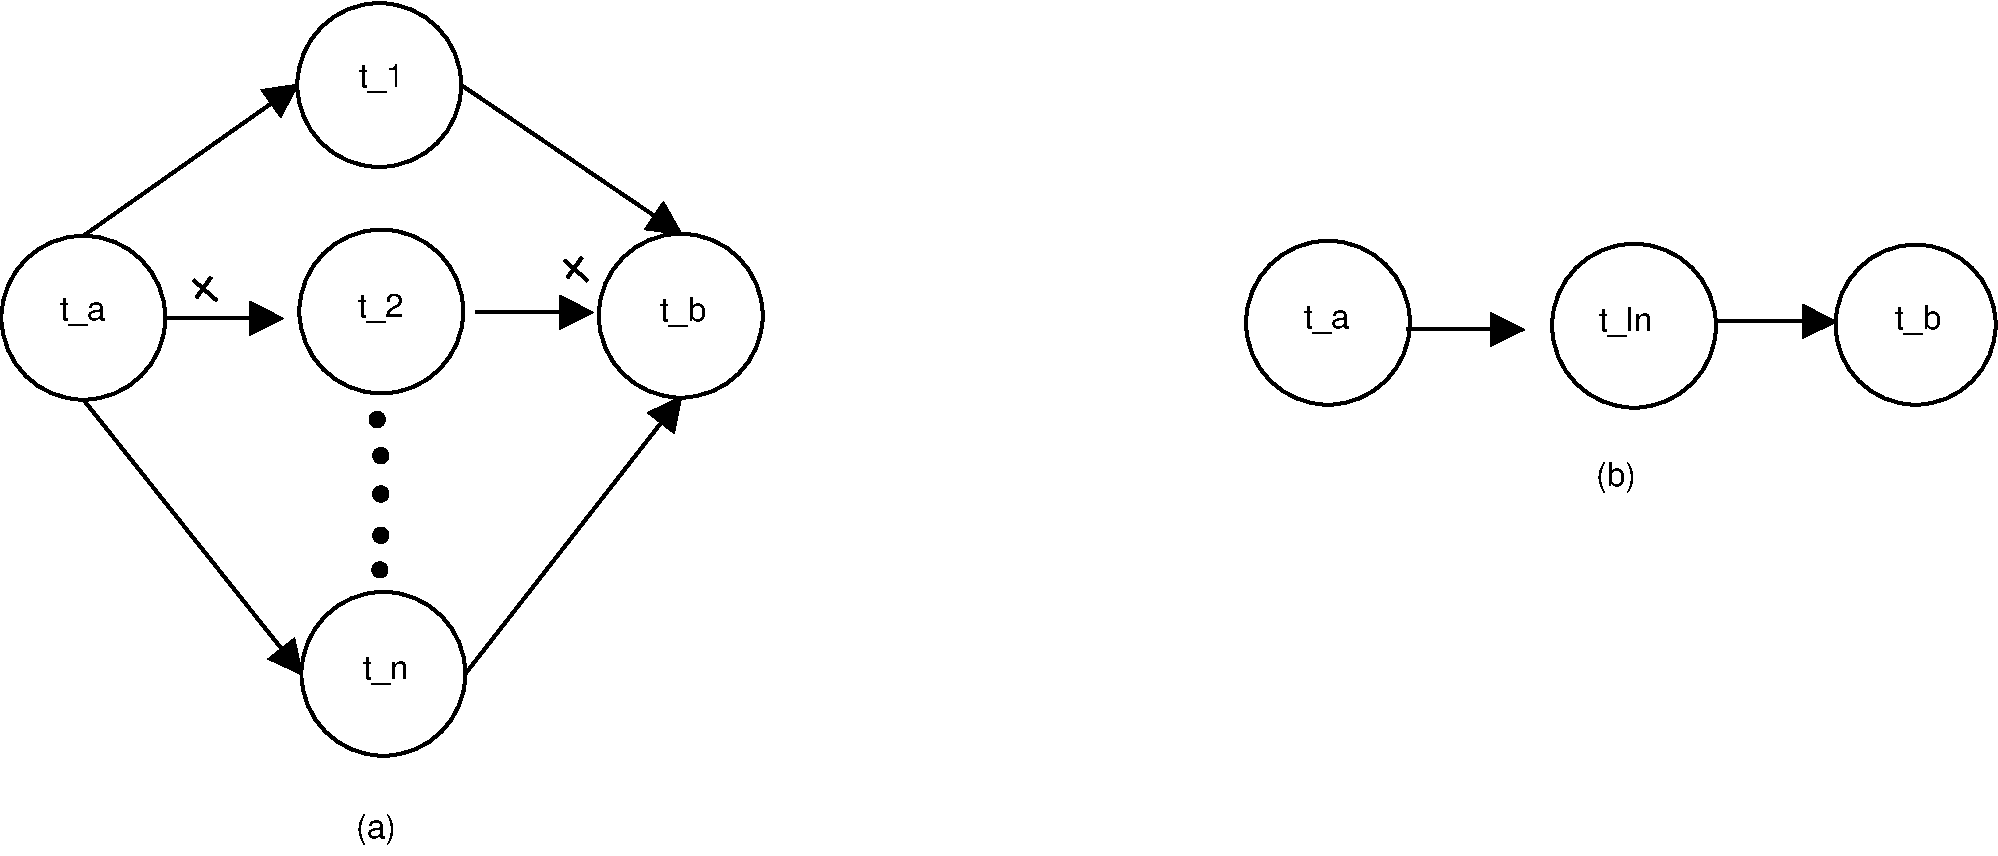
\includegraphics[scale=0.27]{drawings/parallel_reduction.pdf}
	}
	\caption{Reduction of parallel tasks(reproduced from \cite{Cardoso2004Quality}). For additive QoS, the attributes are summed up, while for multiplicative QoS, the attributes are multiplied together\label{fig:parallel_reduction}}
\end{figure}

Thus, if the cost for each of the parallel tasks ($t_{1}...t_{n}$) is $5$ units each, then the cost of $t_{N}$ would be $5 * n$. Likewise, if the reliability for (say) three tasks ($t_{1}...t_{3}$) is $0.9$ each, then the reliability for $t_{N}$ would be $0.729$. Similar reduction formulae \cite{Cardoso2004Quality} are used for other types of tasks, such as sequential tasks, loop tasks, conditional tasks, etc.


\subsubsection{Decomposing End-to-End constraints\label{decomposing_constraints}} QoS constraints are usually specified on an application-wide basis. That is, performance for an entire application (end-to-end) or a cost constraint that must be met. To achieve these constraints in a decentralized manner, we decompose the global constraints that the application imposes, into local ones (the reverse process of SWR). Local constraints can can be handed over to individual BuyerAgents. Amongst the three type of QoS that we consider, the last two types of constraints (boolean and categoric) do not need to be decomposed at all. They are given to all agents, as is. For example, if \texttt{all services must use encryption} is a constraint, then every agent can be given the constraint, without any processing. On the other hand, constraints like \texttt{cost of all services $< C$} need to be decomposed on a per-Agent basis. Numeric constraints are decomposed, as shown in \ref{algo_decomposing_numeric_constraints}

\begin{algorithm}
 \DontPrintSemicolon
 \KwData{Numeric Constraints Limit}
 \KwResult{Numeric Constraints Decomposed}
 \Begin{ 
 \ForEach{$Agent\ a$}{
 	Find list of markets $(M)$ corresponding to $a_{f_{x}}$\;
 	Choose $m \in M$\;
 	Register in $m$\;
 	$a \longleftarrow m_{last\_k\_transactions}$\;
 	\ForEach{$\omega \in NumericConstraints$}{
		calculate $a^{\omega\_m}_{low}, a^{\omega\_m}_{median}, a^{\omega_m}_{high}$ \;
	}
  }
  \ForEach{$\omega \in NumericConstraints$}{
  	Apply SWR $\longleftarrow \langle \omega^{f_{1}}, \omega^{f_{2}}, \omega^{f_{3}} \ldots \rangle$\;
  	\If{$constraintMet$}{
		\ForEach{$Agent\ a$}{
			$a_{bid}^{\omega} \propto {SWR}^{\omega}$\;
		}
  	}
  	{
	  	Choose different $m$\;
  		\If{$allMarketsExhausted$}{
  			TerminateWithFailure\;
  		}
  	}
 }
}
 \caption{Decomposition of Numeric Constraints \label{algo_decomposing_numeric_constraints}}
\end{algorithm}

\subsection{Adaptation Using Bid Generation}\label{bid_generation}

\textit{Bids} are the mechanism by which BuyerAgents explore the search space of QoS-cost combinations that are available. Depending on the \textit{bids}, potential transactional matches are identified by the MarketAgent. Thus, there needs to be a systematic way to generate bids, that not only meet the application's QoS requirements, but also explore the space of possible matches. The relevant parts that go into a Bid are given in table \ref{tbl:bid_elements}.

\begin{table*}
\centering
\begin{tabular}{p{7cm}p{7cm}}
\toprule
Category & Value \\
\midrule
Types of QoS attributes & Boolean, Categoric  and Numeric \\
Constraint on each attribute & Hard, Soft \\ 
Direction on each attribute & Maximize, Minimize, N.A. \\ 
Bid\_Price & Numeric \\
\bottomrule
\end{tabular}
\caption{Elements in a Bid \label{tbl:bid_elements}}
\end{table*}

The most important part of deciding on a value for a QoS attribute, in a Bid is the constraint on each attribute. If the constraint is hard, then, in each of the generated bids, the value inserted into the bid will remain the same. Else, the value inserted into the bid is varied. The varied values depend on the type of QoS attribute. The rules for generating QoS values, on the basis of type of attribute are as follows:

\paragraph{Boolean} In case of soft constraints, two bids will be generated for a particular QoS attribute. For example, for QoS attribute \textit{SSL support}, one bid is generated with the value: \textit{yes} and another with the value: \textit{no}

\paragraph{Categoric} In case of soft constraints, the number of bids will depend on the number of acceptable alternatives. For example, for QoS attribute {framerate}, the acceptable alternatives are: \textit{24fps} and \textit{32fps}. Therefore, two bids will be generated. 

\paragraph{Numeric} In case of soft constraints, the number of bids will be three. That is, the BuyerAgent makes one bid at its target value, one at the median value obtained from the market, and the last one at the mid-point between the target and the median value.

Thus, the total number of bids that a buyer generates is given by:
\setlength{\arraycolsep}{0.0em}
\begin{eqnarray}
Num(buyer_{bids})&{} = &{ }2 * Num(BooleanQoS)\nonumber\\
						  && *{ }  Num(AcceptableAlternatives)\nonumber\\
						  && *{ } 3 * Num(NumericQoS)
\end{eqnarray}
\setlength{\arraycolsep}{5pt}

Thus, if a BuyerAgent has the QoS and preferences as given in table \ref{tbl:sample_qos_preferences}:

\begin{table*}
\centering
\begin{tabular}{lcccc}
\toprule
\textbf{Name} & \textbf{Type} & \textbf{Median} & \textbf{Target} & \textbf{Direction} \\ 
\midrule
SSL Support & Boolean & No & Yes/No & N.A. \\ 
FrameRate & Categoric & 24fps & 24fps, 32fps & Maximize \\ 
Latency & Numeric & 99ms & 95ms	& Minimize \\ 
Budget & Hard Constraint & (From Market) &  100 & N.A. \\ 
\bottomrule
\end{tabular}
\caption{QoS preferences for a BuyerAgent \label{tbl:sample_qos_preferences}}
\end{table*}

The total number of bids that it would generate would be:
\begin{eqnarray} \label{eqn:num_generated_bids}
Num(buyer_{bids}) &=& 2 * Num(SSL Support)\nonumber\\
					&&  * Num(FrameRate)\nonumber\\
					&& 	* 3 * Num(Latency)\nonumber \\
		            &=& 2 * 2 * 3  \nonumber \\
        		    &=& 12 \nonumber
\end{eqnarray}

\begin{table*}
\begin{minipage}[b]{0.5\linewidth}
\begin{tabular}{p{3cm}c}
\toprule
Attribute & Value \\
\midrule
Bid-Price & 80 \\ 
SSL & Yes \\ 
Framerate & 24fps \\ 
Latency & 99 \\ 
\bottomrule
\end{tabular}
\end{minipage}
\begin{minipage}[b]{0.5\linewidth}
\begin{tabular}{p{3cm}c}
\toprule
Attribute & Value \\
\midrule
Bid-Price & 80 \\ 
SSL & No \\ 
Framerate & 32fps \\ 
Latency & 99 \\ 
\bottomrule
\end{tabular}
\end{minipage}
\caption{Sample Bids}
\end{table*}

\subsection{Decentralized Decision-Making Using Ask-Selection}\label{ask_selection}
According to the market mechanism that we have outlined, a BuyerAgent can make multiple bids. This is how it searches the space of possible services that it could get, for its stated budget. Now, there might be multiple asks in the market that match these multiple bids. The market mechanism now moves on to its second-stage, where the BuyerAgent has to select amongst the possible transactions. Given that the mechanism for bid generation precludes bids that will violate hard constraints, it is safe to assume that none of the possible transactions will violate the application's hard constraints either. The task facing the BuyerAgent, is to choose amongst the possible transactions, in such a way that the decision maximizes the possible benefits, while taking care to minimize the possible downsides. We use a multiple criteria decision making approach called PROMETHEE\cite{Brans1985Preference}\\
The BuyerAgent needs to rank all the CandidateServices, that have been returned by the MarketAgent, as a potential transaction. Thus, for a transaction set ($TS$), the BuyerAgent needs to select one CandidateService that it will actually transact with. Depending on the number of QoS attributes, the preference of CandidateService $a$ over CandidateService $b$ is calculated by aggregating the preferences over each QoS attribute (and its weightage). The aggregate preference value of a CandidateService is calculated as:
\begin{equation}
\pi(a,b) = \sum_{i=1}^{n} P_{i}(a,b)w_{i}
\end{equation}

Using this preference value, each CandidateService is ranked \textit{vis-a-vis} the other CandidateServices in the possible transaction set. Ranking is done by calculating the positive outranking flows and the negative outranking flows:
\begin{equation}
\o^{+}(a) = \sum_{x \in TS}\pi(a,x)
\label{positive_outranking}
\end{equation}

\begin{equation}
\o^{-}(a) = \sum_{x \in TS}\pi(x,a)
\label{negative_outranking}
\end{equation}

Finally, the net outranking flow is created to get a complete ranking of all the CandidateServices:
\begin{equation}
\o(a) = \o^{+}(a) - \o^{-}(a)
\label{net_outranking}
\end{equation}

Choice of the CandidateService is based on the following heuristic:
	\begin{enumerate}
		\item Based on the net outranking flow, choose the best CandidateService. 
		\item If there is a tie, choose the cheaper CandidateService out of the pool of best CandidateServices
		\item If using cost still leads to a tie, choose randomly amongst pool of best CandidateServices
	\end{enumerate}

\subsection{A Worked-out Example}
Suppose that the MarketAgent returns the 4 Asks (as shown in table\ref{tbl:potential_transactions}), as possible transaction matches:
\begin{table*}
\centering
\subfloat[][CandidateService A]{
\begin{tabular}{p{3cm}c}
\toprule
Attribute & Value \\
\midrule
Ask-Price & 74 \\ 
SSL & Yes \\ 
Framerate & 24fps \\ 
Latency & 99 \\ 
\bottomrule
\end{tabular}
}
\qquad
\subfloat[][CandidateService B]{
\begin{tabular}{p{3cm}c}
\toprule
Attribute & Value \\
\midrule
Ask-Price & 78 \\ 
SSL & Yes \\ 
Framerate & 24fps \\ 
Latency & 95 \\ 
\bottomrule
\end{tabular}
}
\qquad 
\subfloat[][CandidateService C]{
\begin{tabular}{p{3cm}c}
\toprule
Attribute & Value \\
\midrule
Ask-Price & 80 \\ 
SSL & No \\ 
Framerate & 24fps \\ 
Latency & 90 \\ 
\bottomrule
\end{tabular}
}
\qquad
\subfloat[][CandidateService D]{
\begin{tabular}{p{3cm}c}
\toprule
Attribute & Value \\
\midrule
Ask-Price & 76 \\ 
SSL & Yes \\ 
Framerate & 32fps \\ 
Latency & 92 \\ 
\bottomrule
\end{tabular}
}
\caption{Asks returned by MarketAgent as potential transactions \label{tbl:potential_transactions}}
\end{table*}

Ranking amongst multiple asks is done on a per-QoS attribute basis. That is, each ask is ranked on each QoS attribute. Depending on the type of QoS attribute, the criteria used from PROMETHEE is shown in table \ref{tbl:qos_promethee_mapping}

\begin{table}
\centering
\begin{tabular}{ll}
\toprule
QoS Attribute Type & PROMETHEE Criterion Type \\
\midrule
Boolean & Usual Criterion \\
Categoric & Quasi-Criterion \\
Numeric & Criterion with Linear Preference \\
\bottomrule
\end{tabular}
\caption{QoS Attribute to PROMETHEE Criterion Mapping \label{tbl:qos_promethee_mapping}}
\end{table}

Table \ref{tbl:qos_promethee_mapping} effectively means that CandidateServices will be evaluated on their QoS attributes as follows:
	\begin{enumerate}
		\item In case of a boolean attribute, a CandidateService A will be preferred over CandidateService B, if it has a desired boolean value, while the other doesn't. Else, there is no preference.
		\item In case of a categoric attribute, a CandidateService A will be preferred over CandidateService B, if the categoric value of A is better by $k$ over the categoric value of B. Else, there is no preference. The value of $k$ is adjusted based on whether the attribute is a hard constraint or a soft constraint. For hard constraints, $k$ is taken to be zero, \textit{i.e.}, the CandidateService with the better categoric value (higher if the attribute is to be maximized, minimized otherwise) is strictly preferred over the other. 
		\item In case of a numeric attribute, a CandidateService A will be increasingly preferred over CandidateService B, as the difference between their numeric value approaches some $m$. After $m$, A is strictly preferred. Again, the value of $m$ is adjusted based on whether the attribute is a hard constraint or a soft constraint. 
	\end{enumerate}
	
	The preference functions for the three QoS attributes can be given as follows:
	
	\begin{equation}
		P_{ssl}(x) = \begin{cases} 0 &\mbox{if } x = (ssl=no),\\ 
							1 &\mbox{if } x = (ssl=yes) \end{cases}
			\label{pref_ssl}
	\end{equation}

	\begin{equation}
		P_{framerate}(x) = \begin{cases} \frac{1}{32}x &\mbox{if } x < 32fps,\\ 
										1 &\mbox{if } x \geq 32fps \end{cases}
			\label{pref_framerate}										
	\end{equation}
	
	\begin{equation}
		P_{latency}(x) = \begin{cases} 0 &\mbox{if } x > 103ms,\\ 
									   \frac{1}{2}	 &\mbox{if } 103 > x > 95ms, \\
										1 &\mbox{if } x \leq 95 \end{cases}
			\label{pref_latency}
	\end{equation}
	
Based on the preference equations \ref{pref_ssl}, \ref{pref_framerate} and \ref{pref_latency}, we can calculate the relative values of the 4 CandidateServices, as given in table \ref{tbl:outranking_table}
	\begin{table}[htbp]
		\centering
		\caption{Values of $\pi(x_i, x_j)$ \label{tbl_ranking_values}}
		\rowcolors{2}{gray}{}
		\begin{tabular}{c|cccc}
		\toprule
		  & A & B & C & D \\
		\midrule
		A & --- & 0 + 0 + (-0.5) & 1 + 0 + (-0.5) & 0 + (-0.25) + (-0.5) \\
		B & 0 + 0 + 0.5 & --- & 1 + 0 + 0 & 0 + (-0.25) + 0 \\
		C & (-1) + 0 + 0.5 & (-1) + 0 + 0 & --- & (-1) + (-0.25) + 0 \\
		D & 0 + 0.25 + 0.5 & 0 + 0.25 + 0 & 1 + 0.25 + 0 & --- \\
		\bottomrule
		\end{tabular}
	\end{table}
Once we have a relative per-attribute value, we can calculate the outranking values based on equations \ref{positive_outranking},\ref{negative_outranking} and \ref{net_outranking}, as shown in table \ref{tbl:outranking_table}

	\begin{table}[htbp]
		\centering
		\renewcommand{\arraystretch}{1.5}
		\begin{tabular}{c|cccc}
		\toprule
		   			& A & B & C & D \\
		\midrule
			$\o^{+}$	& 0.5 & 1.5 & 0 & 2.25 \\
			$\o^{-}$	& 1.25 & 0.25 & 2.75 & 0 \\
			\hline
			$\o$		& -0.75 & 1.25 & -2.75 & 2.25 \\
		\bottomrule
		\end{tabular}			
		\caption{Calculation of outranking values \label{tbl:outranking_table}}
	\end{table}
It is clear from table \ref{tbl:outranking_table} that CandidateService D is the best amongst the potential transactions and CandidateService C is the worst. The BuyerAgent now accepts the transaction with CandidateService D and rejects all the others. 

\subsection{Post-Transaction}
The BuyerAgent reports back to the ApplicationAgent, the cost and QoS being made available for the transaction. The ApplicationAgent then performs a SWR calculation to ensure that the QoS of the service being bought, does not violate any of the application's end-to-end constraints. Note that the ApplicationAgent needs to calculate SWR for the numeric constraints only. The other types of constraints (boolean and categoric) are specified in the bid prepared by the BuyerAgent, and therefore do not need checking. This greatly reduces the computational effort required on the part of the Application agent. The best case scenario, from a computational perspective, is when all the QoS attributes of the Application are either boolean or categoric. However, in the worst case scenario, all the QoS attributes that the ApplicationAgent is  interested in, could be numeric. In this case, it has to perform an SWR calculation for each of the QoS attributes and the distribution of computation to BuyerAgents is minimal.\\

In Figure \ref{fig:cda_activity_diagram}, we show the various steps in the CDA  as activities carried out by the principal agents.
 
 \begin{figure}[h]
	\centering
	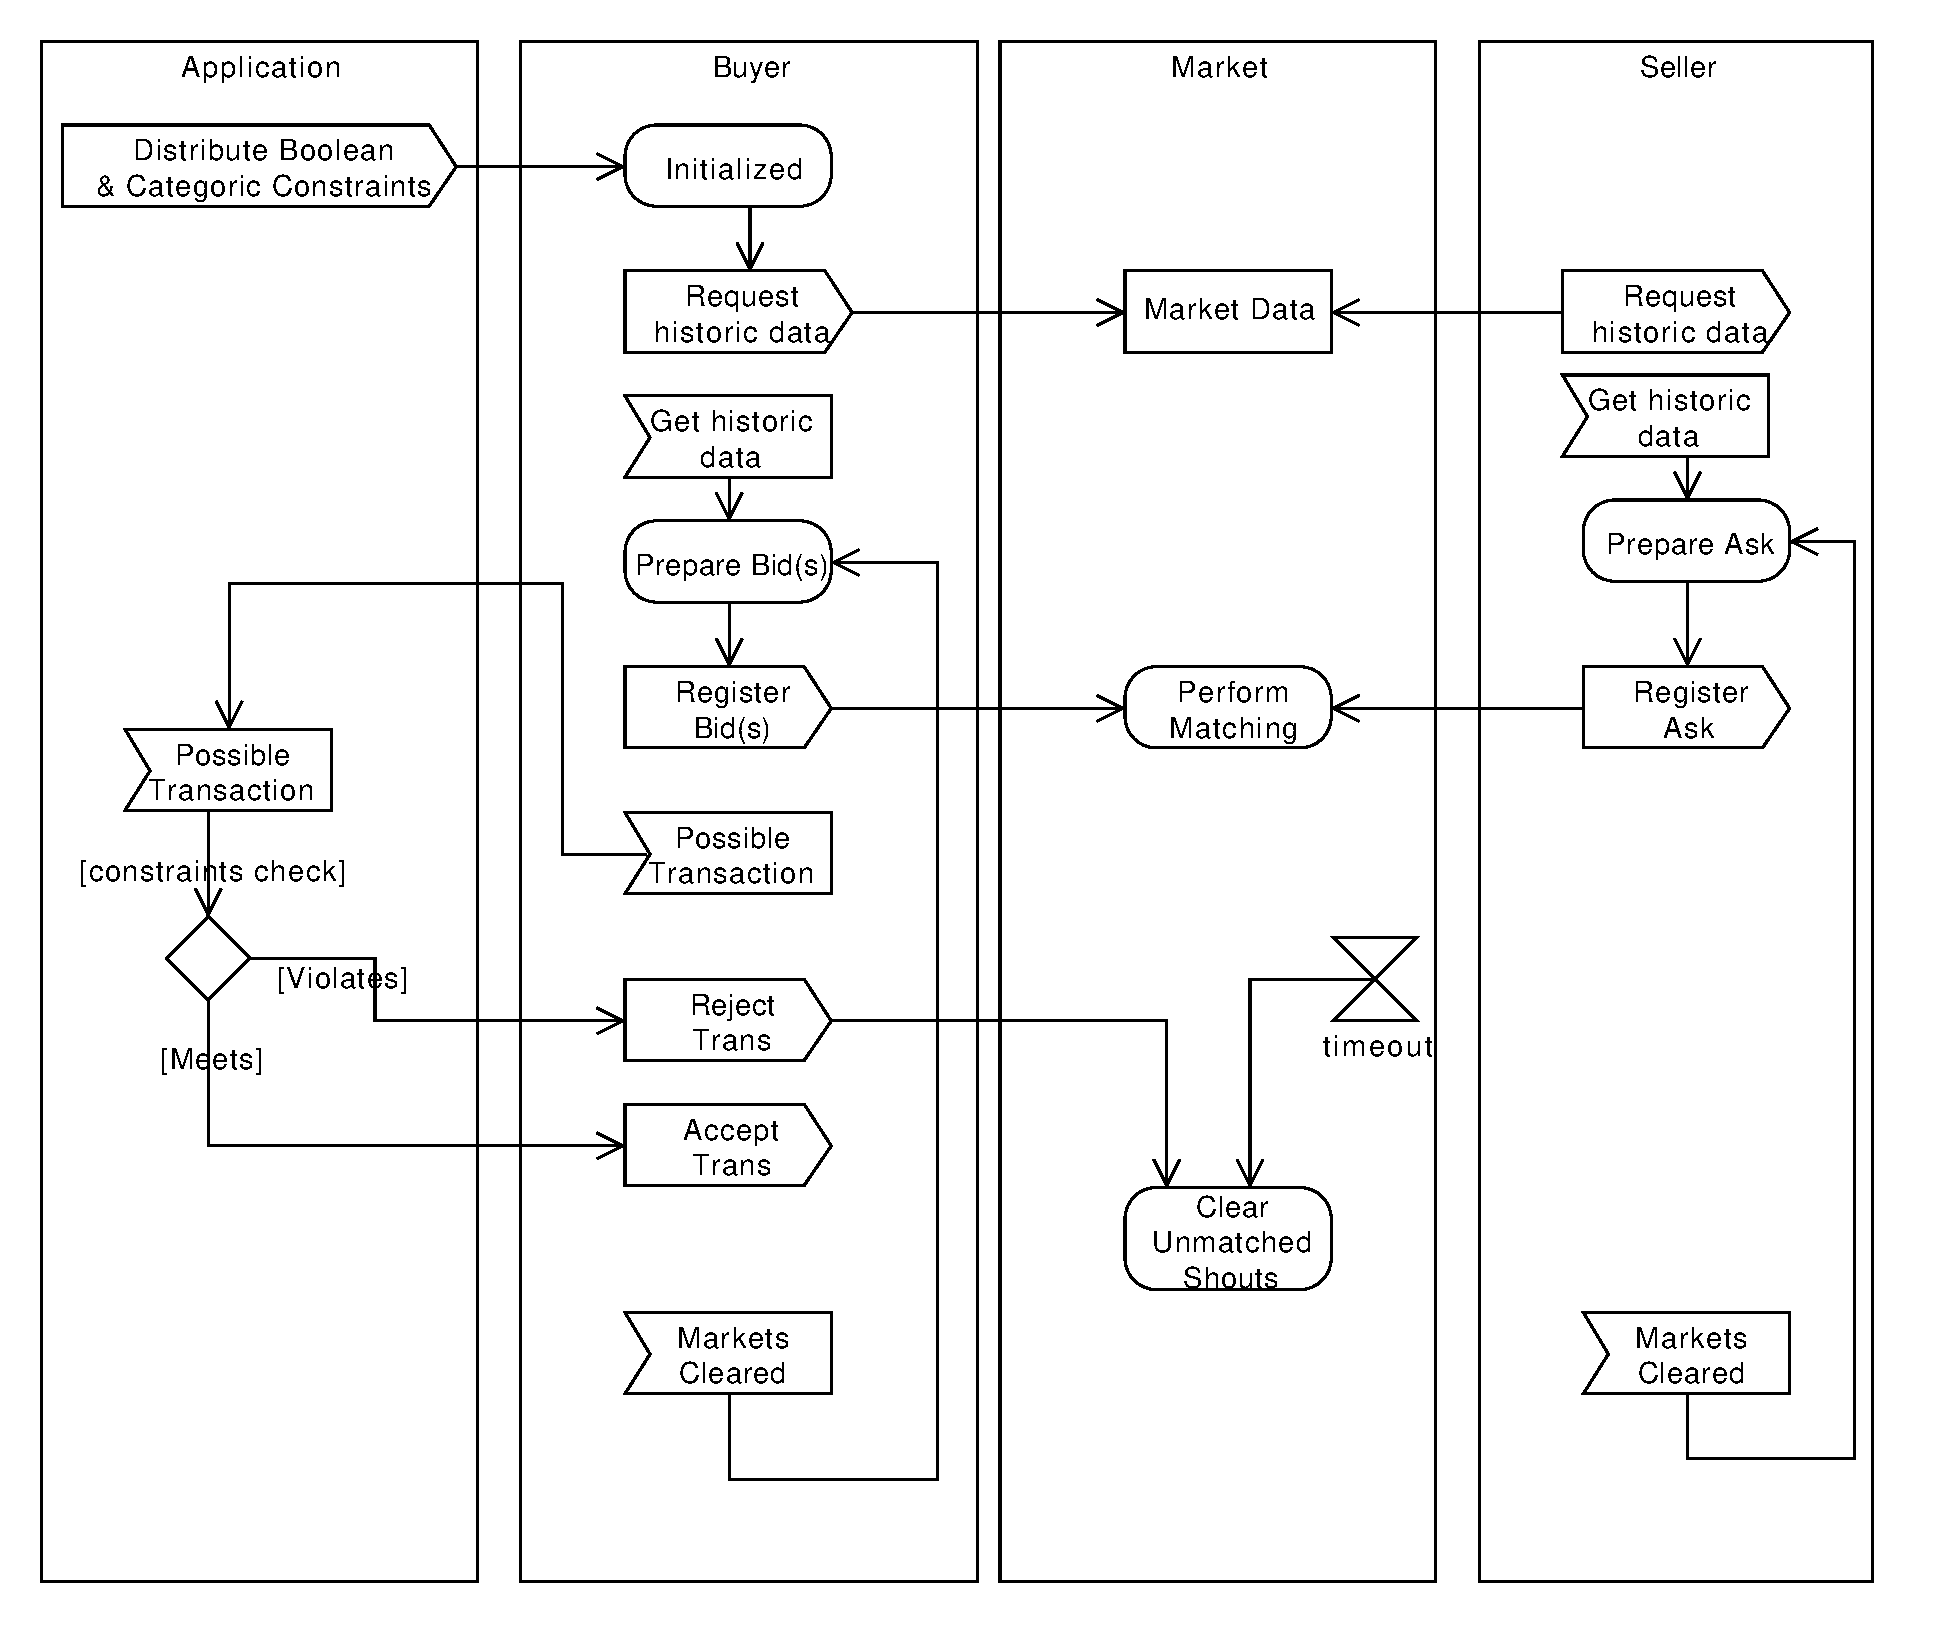
\includegraphics[scale=0.3]{drawings/CDA_Activity_Diagram.pdf}
	\caption{Activity diagram for principal agents}
	\label{fig:cda_activity_diagram}
\end{figure}	

\subsection{Re-starting Conditions}
Once an application reaches a satisfactory level of QoS, all its agents will withdraw from the market. The agents will re-enter the market, only in case of an \textbf{adaptation stimuli}. There are two kinds of adaptation stimuli:
	\begin{enumerate}
	    \item External Stimuli: When a QoS violation is detected at any of the CandidateService, the ApplicationAgent informs the BuyerAgent that it needs to re-start its search for a new CandidateService. This event is not propagated to all the BuyerAgent, but only to the particular one responsible for that AbstractService.
	     \item Internal Stimuli: When the application's end-to-end QoS target or available budget changes, the ApplicationAgent informs all of its BuyerAgents, and restarts the adaptation. The agents stay in the adaptation phase, until the stopping criteria are met.
	\end{enumerate}
Both these stimuli occur at different time scales. The external check for QoS violation is a continuous check and concerns itself with performance of the web-service across relatively shorter periods of time. The internal stimulus, on the other hand, typically happens when budgets for operation change drastically or external events cause change in performance or reliability requirements. This happens at relatively rarer intervals. Hence, typically once an application reaches close to its desired level of QoS, the BuyerAgents stop trading.

%\subsubsection{Buyer}
%The Buyer is a trading agent that buys a web-service for an Application, \textit{i.e.,} it trades in a market for a specific $f_x$. Each web-service, available in $f_x$, exhibits the same QoS ($\omega \in QoS$). The only differentiating factor is the degree to which that is exhibited  ($ \omega_{i} \in \mathbb{R}_{0}^{1} $). Hence, if an application has $K$ QoS that it is concerned about, then the QoS that it gets for each of the $f_{x}$ that it buys is:
%	 \begin{equation}
%	  \Omega^{f_{x}} = \langle \omega_{1}^{f_x}, \omega_{2}^{f_x}, \omega_{3}^{f_x}, \ldots, \omega_{K}^{f_x} \rangle \label{eq:exhibited_qa}
%	 \end{equation}
%
%The amount that the buyer is prepared to pay is called the \textsl{bid price} and this is necessarily \textit{less than or equal to} the $B_{f_x}$, where $B_{f_x}$ is the budget available with the buyer. The combination of $\Omega$ demanded and the \textsl{bid price} is called a \textsl{Bid}.
%
%\subsubsection{Seller}
%Each seller is a trading agent, selling a web-service that exhibits the QoS required in (\ref{eq:exhibited_qa}). The degree to which each qa($\omega$) is exhibited in each $f_x$ being sold, is dependent on the technological and economic cost of providing it. For example, if the cost of providing $f_x$ with $\Omega = \langle 0.5, 0.6 \rangle$ is low, then there will be many sellers providing $f_x$ with a low \textsl{ask price}. Conversely, if the cost of providing $f_x$ with $\Omega = \langle 0.8, 0.9 \rangle$ is high, then the \textsl{ask price} will be high. An individual seller's \textsl{ask price} can be higher or lower based on other factors like number of sellers in the market, the selling strategy etc. For the purpose of this paper, we consider only a single constraint between cost and \textsl{ask price}, where the \textsl{ask price} is always \textit{greater than or equal to} the cost. The combination of $\Omega$ and \textsl{ask price} is called the \textsl{Ask}. Every service is sold for a pre-specified $n$ calls, \textit{i.e.,} a purchase of a service entitles the buyer to make $n$ (market specified) calls to that service. Provenance regarding the actual usage of the service, can be easily established through the use of authentication keys, etc. 
%
%\subsubsection{Market} 
%A market is a set of buyers and sellers, all interested in the same functionality $f_x$. The factors differentiating the traders are:
%	\begin{itemize}
%	 \item \textbf{$\Omega$:} The combination of $\langle \omega_{1}, \omega_{2}, \ldots \omega{k}\rangle$
%	 \item \textbf{\textsl{Price:}} Refers to the \textsl{bid price} and \textsl{ask price}. The buyers will not pay more than their respective \textsl{bid price} and the sellers will not accept a transaction lower than their respective \textsl{ask price}. 
%	\end{itemize}
%
%The mechanism of finding a matching buyer-and-seller is the \textit{continuous double auction}(CDA). A CDA works by accepting offers from both buyers and sellers. It maintains an orderbook containing both, the \textsl{bids} from the buyers and the \textsl{asks} from the sellers. The bids are held in descending order of price, while the asks are held in ascending order, \textit{i.e.}, buyers willing to pay a high price and sellers willing to accept a lower price are more likely to trade. When a new \textit{bid} comes in, the offer is evaluated against the existing \textit{asks} in the book and a transaction is conducted when the price demanded by the \textit{ask} is lower than the price the \textit{bid} is willing to pay \textbf{and} all the QoS attributes in $\Omega$ of the ask are \textit{greater than or equal to} all the QoS attributes in the $\Omega$ of the \textit{bid}. After a transaction, the corresponding \textit{bid} and \textit{ask} are cleared from the orderbook.
%\begin{figure}
%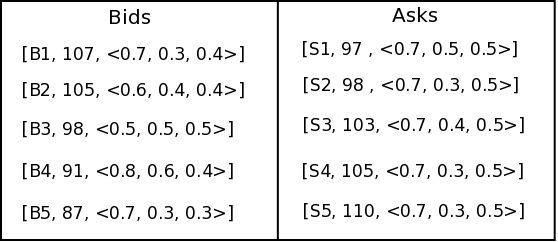
\includegraphics[scale=0.31]{drawings/orderbook.png}
%\caption{Orderbook at time $t_{0}$}
%\label{orderbook}
%\end{figure}
%Figure \ref{orderbook} shows the state of the orderbook at some time \textit{$t_{0}$}. Maximizing the number of transactions would lead to a possible set like: $[B1-S4, B2-S3, B3-S1]$. Calculating this optimal set, however, quickly becomes infeasible as the number of bids and asks increase, since the number of pairwise comparisons needed increases exponentially.  With a CDA, the set of transactions is: $[B1-S1, B2-S3]$. This is so because a CDA evaluates bids and asks, as they come in and the first possible match is set up as a transaction. Thus, $[B1-S1]$ is immediately matched and removed from the orderbook, and then $[B2-S3]$ is matched.  Since this procedure is carried out for every offer (\textit{bid/ask}) that enters the market, the only bids and asks that remain on the orderbook are those that haven't been matched (figure \ref{orderbook-after-one-pass}). This procedure is much faster, and easily parallelizable. Although counter-intuitive, it has been shown that even when buyers and sellers have Zero-Intelligence, the structure of the market allows for a high degree of allocative efficiency \cite{Gode1993Allocative}. Zero-Intelligence refers to a strategy, where the agents involved, do not consider any historical information about trades, and nor do they possess any learning mechanism. Thus, Zero-Intelligence marks the lower limit of the efficiency of a CDA market.
%\begin{figure}
%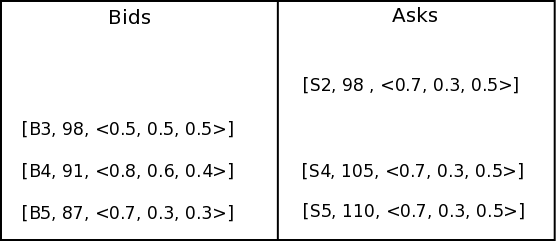
\includegraphics[scale=0.31]{drawings/orderbook-after-one-pass.png}
%\caption{Orderbook at time $t_{1}$}
%\label{orderbook-after-one-pass}
%\end{figure}

%TODO: INSERT MODIFIED CDA: 2-STEP: 1 FOR TRADING AND 2 FOR APP TO CALCULATE BEFORE COMMITMENT. REFERENCE RAMCHURN'S PAPER ON 2-STEP CDA FOR EVIDENCE OF BETTERNESS

%\subsubsection{Applications}
%The Application is a composition of services from different markets. At the agent-level, the application agent communicates with each of the buying agents ($f_{x} \in F_{x}$) and communicates a budget ($B_{f_{x}}$). The buyer then initializes itself with a random $\Omega^{f_x}$ and starts trading. The adaptation occurs through the revision of bids, that happen after each round of trading. After each round of trading, depending on the $\Omega$ obtained by the buyer, the Application has procured a total QoS that is calculated, using Stochastic Workflow Reduction\cite{Cardoso2004}.\\
%Buying and using a web-service involves many costs, and these must be compared against the projected utility gain to decide whether it is worthwhile to switch. These may be enumerated as:
%	\begin{itemize}
%	 \item \textit{Buying Cost:} The price of purchasing the web-service for \textsl{n} calls ($p_{f_x}$)
%	 \item \textit{Transaction Cost:} The amount to be paid to the market, for making the transaction ($t_{f_x}$)
%	 \item \textit{Switching Cost:} Every contract with a web-service would incorporate the total number of calls or the time for which the service is available, at the transaction price. If the application wants to break this contract, it would have to pay a penalty to the supplier. This amount of penalty to be paid is the switching cost ($s_{f_x}$). In real life, the switching cost would include other variables like opportunity cost, penalties levied by the application's consumers for loss of service, etc. Since these are more difficult to measure, we restrict ourselves to the directly observable values, such as penalty for breaking a contract.
%	 \end{itemize}
%Thus, the total cost that the application must consider is:
%	\begin{equation}\label{eq:total_cost} 
%	 TC_{f_x} = p_{f_x} + t_{f_x} + s_{f_x}
%	\end{equation}
%	 
%We assume that, for every application there exists a function that maps $TC_{f_x}$ to an equivalent $\Omega^{f_x}$. The application could easily buy the best possible web-service(s) available, if it was prepared to spend a large amount of money. However, in reality, every application is constrained by a budget($B$) that it is willing to spend. The application apportions budget as well as QoS constraints to each of its constituent buyer agents (see algorithm \ref{Initialization}).

%Allocating $B$ amongst the functionalities that it is buying ($f_x \in F_x$) is a matter of strategy and/or the relative importance of each $f_x$. 
%	\begin{equation}
%	 \forall f_{x} \in F_{x}, \sum B_{f_x} = M 
%	\end{equation}

%After every round, the application compares the privately known $\Omega_{f_x}$ with the $\Omega^{b}_{f_x}$ and determines whether to punish/reward the buyer. From this piece of information, the buyer can only guess whether it needs to improve the $\Omega^{b}_{f_x}$ that it obtained or the price that it paid. Once the  $\Omega^{b}_{f_x}$ is close enough to the private $\Omega_{f_x}$, then the application refrains from trading any further, until it changes the privately known $\Omega_{f_x}$. Changing of the private $\Omega_{f_x}$ simulates the change in the environment, which has prompted adaptation by the application. The buyers have to now re-approximate the private $\Omega_{f_x}$.
%Traditionally, a CDA works on a single piece of information, price. However, we modify the bids and asks to be multi-attribute, \textit{i.e.,} each bid also contains the minimum QoS levels that the buyer wants and each ask contains the maximum QoS levels that the seller is willing to provide. Thus, a transaction between a buyer and a seller is now an agreement to provide a certain functionality, at a certain price, at pre-defined QoS levels.
%%After every round of trading, the application calculates the total utility that it obtained after the trades and compares it to the previous utility it had. Depending on whether the utility in the current round is better or worse, the application provides an appropriate feedback to all the buying agents. This allows an agent to realize the effect of its action on the overall utility. It then modifies its bid, accordingly.
%
%In Figure \ref{marketplace}, we see the functionality being composed at the top and the agents below calculating the utility achieved by each trade. The agents are also able to observe the last known transaction price and QoS levels in their markets. This allows them to create bids, that are most likely to result in a trade.


%\subsection{Utility Function}
%A utility function is used to evaluate the QoS obtained by buying a particular web-service. This is done by mapping the QoS values advertised by the web-service onto real values. This involves scaling the QoS values onto a uniform scale, and then applying any weights that the application might indicate as its preference. This mechanism enables QoS attributes that are measured in different units to be treated identically, while calculating utility. Each QoS attribute has a different function, to calculate the end-to-end value. For e.g., while calculating the end-to-end value of performance, we use:
%	\begin{equation} 
%		App_{performance}  = Min_{i \in {1..n}}(a_{i}^{performanceQoS})
%	\end{equation}
%whereas availability is calculated as: 
%	\begin{equation}
%		App_{av} = \prod_{i=1}^{n}(a_{i}^{av})	    
%	\end{equation}
%Thus, in a certain configuration, an application could potentially meet one of its target QoS, while not meeting another. The utility function must be able to reflect this. We use the \textit{Simple Additive Weighting} from \cite{Yoon1995Multiple} for this purpose.  For each application, the target level of QoS is also mapped onto a real value, that is designated as the ideal utility level (IUL) for that application. 
%
%\subsection{Calculating Achieved QoS and Feedback}
% The application agent collects information from each of its buyer agents and calculates the cumulative QoS. It then compares the achieved cumulative QoS against the targetted QoS. On a per-QoS attribute basis, the difference between the achieved and the targetted, is computed and communicated back to the buyer agents.  Intuitively, the easiest way to calculate the application's cumulative QoS is through a central agent that collects QoS information, from each of the buying agents. However, this would lead to dependence on a centralized agent and thus become a bottleneck, in case of applications with a large number of services. We use a gossip-based algorithm, much like Push-Sum\cite{Kempe2003Gossip-Based}, to communicate QoS values. However, unlike Push-Sum, we make the agents gossip information, only to their neighbours' agent (see algorithm \ref{Communication}). A neighbour is defined as a service that is either in the input set or the output set, of a particular service. After each round of gossiping, each agent accumulates its neighbour's QoS information into the QoS calculation function. In the next round of gossip, it sends the new information to other neighbours. Each agent tags its QoS information with its name. This allows agents to recognize if they've seen/sent a particular message before. Agents only send out information that they haven't sent before. When an agent recognizes that it has received all QoS information from all other agents, it runs utility calculation procedures. Feedback is calculated as the difference between the obtained utility and the IUL. The feedback indicates not only the magnitude of the difference, but also the direction. That is, whether the buyer agents have undershot or overshot the target QoS.   
%	
%
%\subsection{Adapting Bids and Asks}
%Bids and Asks form the core of the adaptive process of our mechanism. After an initial start that is influenced by the current QoS values and prices in the market, the buyer agents perform the equivalent of a local search, by means of adjusting the QoS values in their bids. There are many ways to calculate the new QoS value, given a current value and the feedback. We use the least mean squares method (also known as \textit{Widrow-Hoff learning rule})\cite{Haykin2003Least} to adapt the QoS and the price. We use ZIP\cite{Cliff1998Simple}, a fairly simple improvement on the Zero-Intelligence algorithm, that implements the Widrow-Hoff learning rule to perform a gradient descent of the current price (in the ask or bid) to the last transaction price, in the market.  Also, depending on the feedback by the application, each individual buying agent either increases or decreases the QoS attribute values, that it is bidding for. The increase or decrease is determined by the direction indicated in the feedback. The magnitude of change is more difficult to realize. The magnitude indicated in the feedback is a cumulative figure, referring to the difference between target and achieved levels of QoS, for the application. Therefore, each agent changes its QoS bid attributes by a fraction of the magnitude indicated in the feedback (see algorithm \ref{bid_revision}). We use a simple average (magnitude of feedback divided by number of agents in the workflow) to calculate this fraction.\\
%Selling agents also modify their asks, in order to get a better deal for their services. If an agent is able to trade, it increases the price it charges, in the next ask. The sellers also use ZIP to decide on the new charging price(see algorithm \ref{ask_revision}). If the seller is unable to find buyers at a higher price, it drops back to its older price. If it is still unable to find a buyer, then it goes back to the original ask that enabled the agent to transact.\\
%The buyers are constrained by their budget, for the prices that they are willing to pay. The sellers are also constrained by their actual QoS values that they can provide.
%
% 
%\subsection{Stopping Criteria}
%Trading by the agents (and hence adaptation) stops when the application has reached its IUL. Depending on the domain, the application may decide to tolerate a small ($\epsilon$) level of deviation from the IUL. Thus, a satisfactory zone of QoS values is reached which is acceptable to the application. The level of tolerance can be made arbitrarily small or even zero. The stopping criteria can be different for different applications, and indeed, has no restriction whatsoever. Clearly, if it is set injudiciously, the application may either stop adapting too quickly or may never stop adapting. Thus, it becomes an important parameter to tune.
%
%\subsection{Re-starting Conditions}
%There are two conditions where an application that has already reached a satisfactory level of QoS, needs to start adapting again:
%	\begin{enumerate}
%	    \item Internal Stimulus: When a QoS violation is detected at any of the web-services, the application needs to re-start its search for a new web-service to replace the old one. This is not an application-wide adaptation, but localised to a particular web-service
%	     \item External Stimulus: When the application's end-to-end QoS target changes, the application triggers an adaptation in each of its web-services, whereby all the trading agents go through the trading process again, until the stopping criteria is met
%	\end{enumerate}
%Both these events occur at different time scales. The internal check for QoS violation is a continuous check and concerns itself with performance of the web-service across relatively shorter periods of time. The external stimulus, on the other hand, typically happens when budgets for operation change drastically or external events cause change in performance or reliability requirements. This happens at relatively rarer intervals. This implies that once an application reaches close to its desired level of QoS, most of the buying agents stop trading.\\
% 


\subsection{Design and Implementation}
%In \citep{Cheng2009}, the authors comment on the engineering challenges of building a self-adaptive system, and emphasize the fact that the %feedback loop is of utmost importance. 
We call our implementation of the proposed mechanism, \textit{clobmas}(Cloud-based Multi-Agent System). We document \textit{clobmas} using the object-oriented paradigm for all of the internal components of an agent. Thus, we show the static structure of the system through package, component and class diagrams. We show agent-interaction using Agent-UML (AUML).	
\subsubsection{High level Package Diagram} A package diagram shows the coarse-level organization of code in a system, with the packages and sub-packages demarcating the encapsulation of concepts in the system. In figure \ref{fig:package_diagram}, we see that all the agents, \textit{viz.}, buyer, seller, application, market are created and maintained separately from concepts like \textbf{Strategy} and \textbf{Communication}. This independence of packaging also highlights the various axes along which behaviour could be changed. Thus, \textit{clobmas} could change its auction style from a continuous double auction to a double auction with a clearing house, with no effect on the other parts of the system. 

\begin{figure}[H]
\centering
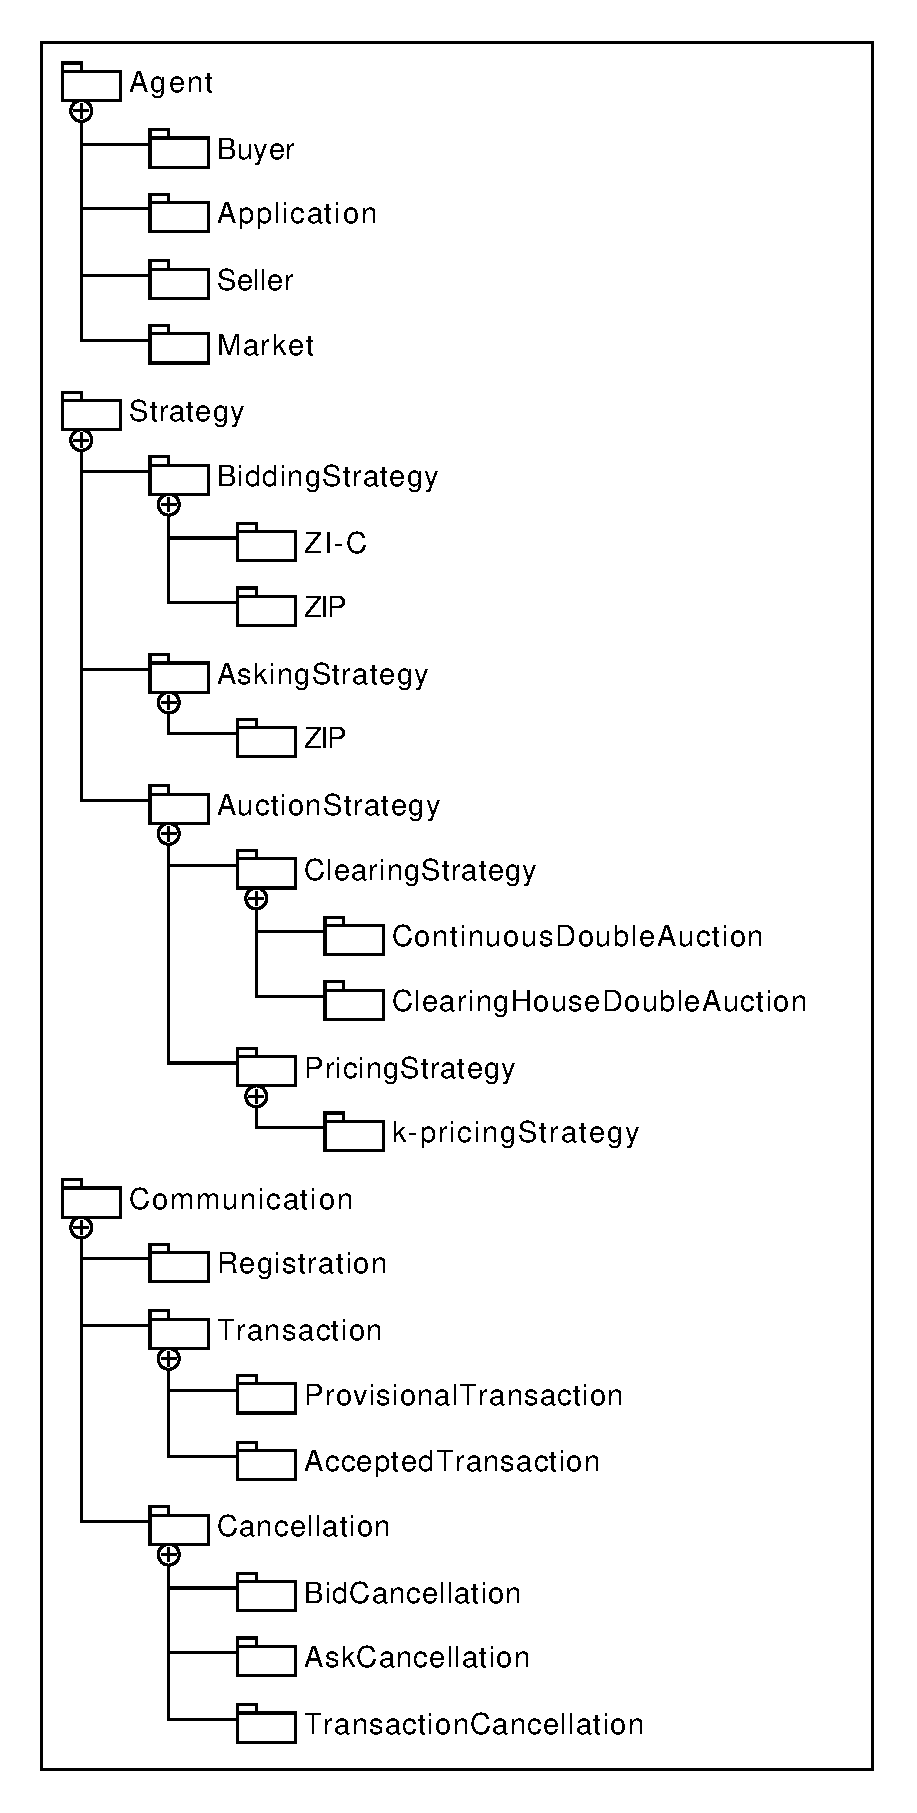
\includegraphics[scale=0.4]{drawings/Agent_Package_Diagram.pdf}
\caption{Package diagram of entities \label{fig:package_diagram}}
\end{figure}

\subsubsection{Architectural Style} The design of our implementation is based on the publish-subscribe architectural style. This style was chosen for its decoupling properties, such that each communicating entity in the system is independent of every other. This fits in well, with our notion of agents acting on the basis of their own goals and their environment, in a decentralized manner. Each type of agent described previously, is both an event publisher and an event subscriber. That is, each ApplicationAgent generates events that describe when the application's QoS constraints have changed, when the budget has changed, etc. These events are subscribed to, by BuyerAgents belonging to that application. The BuyerAgents, for their part, publish events relating to the market that they are registered with. Similarly, the MarketAgents publish events relating to the start of trading, transaction events, etc. The event-based paradigm fits well with the QoS monitoring schemes, as well. Both \cite{Zeng2007Monitoring} and \cite{Michlmayr2009Comprehensive} use events to monitor and communicate SLA violations. 
%
%\begin{figure}[ht]
%	\centering
%	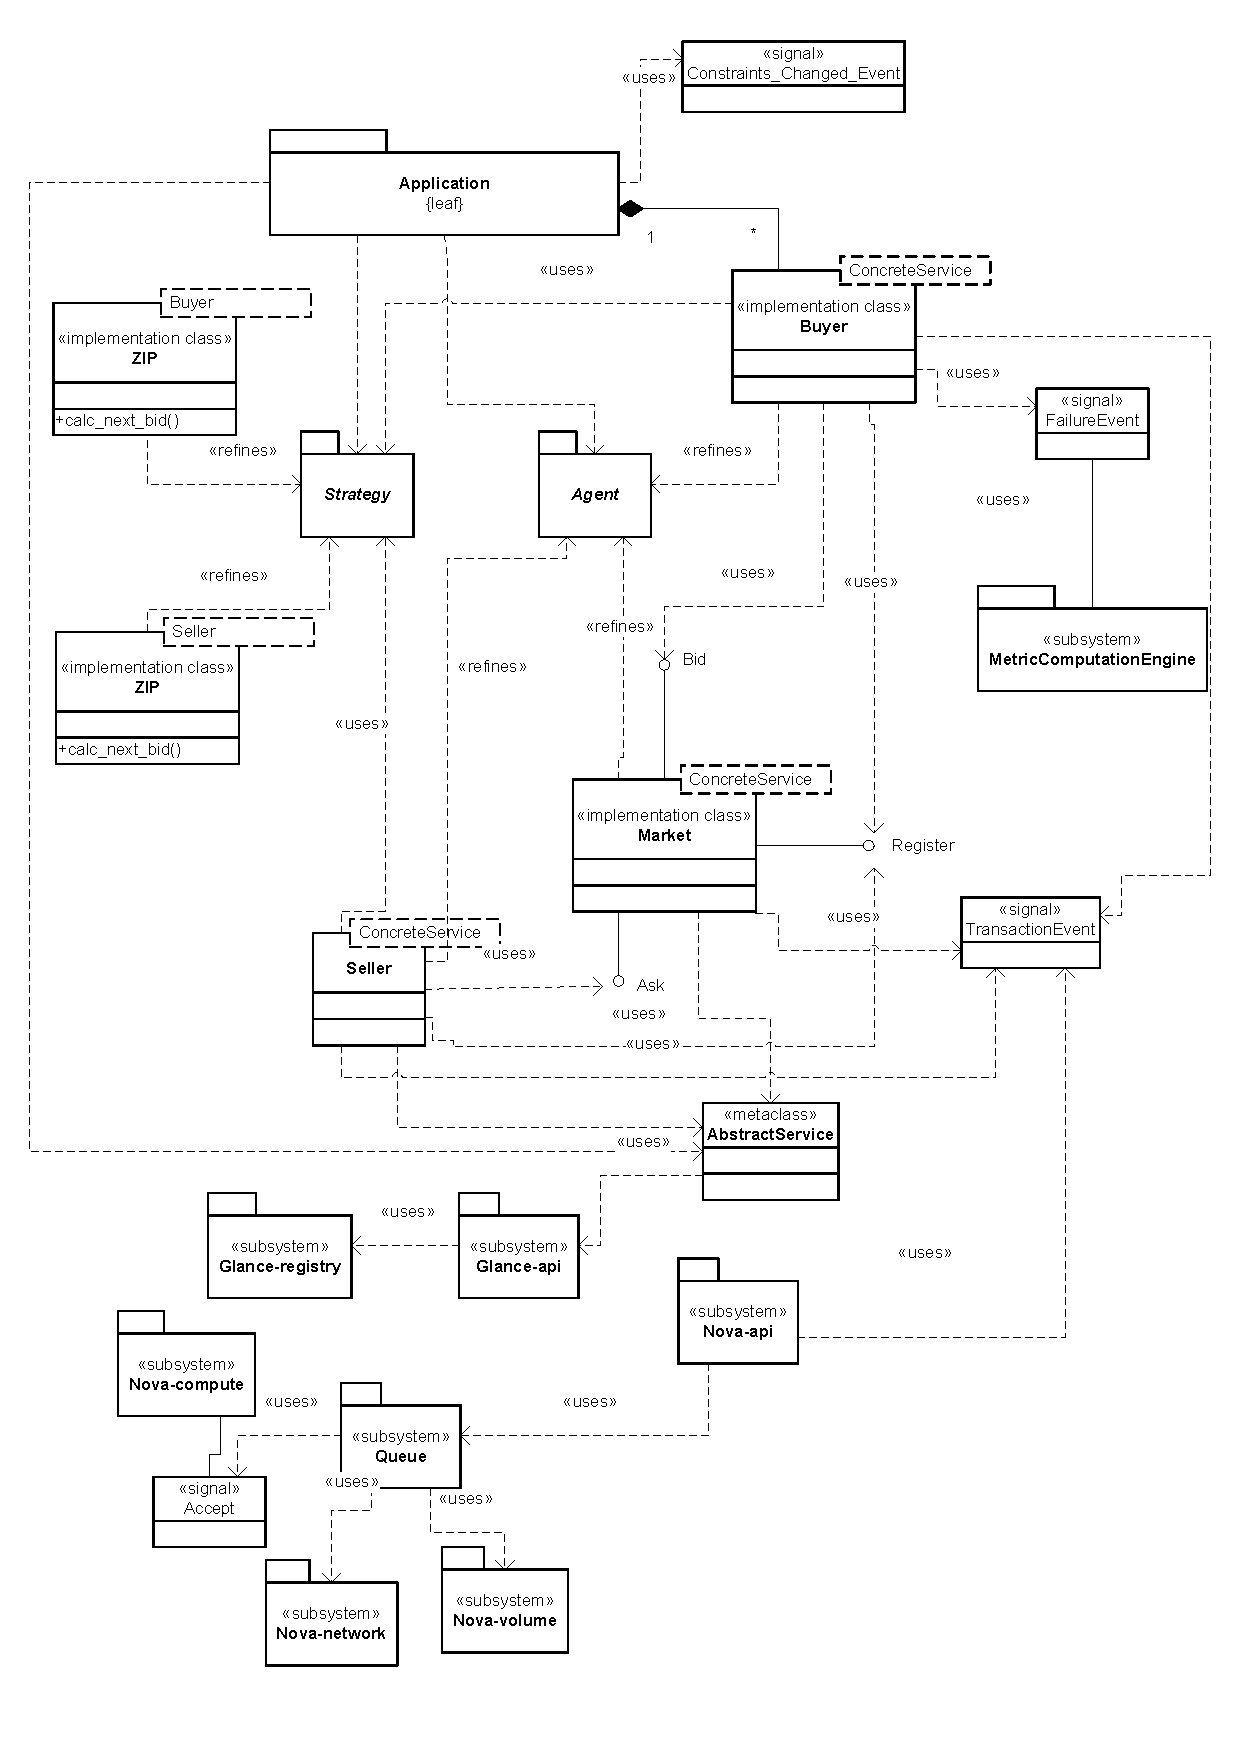
\includegraphics[trim = 30mm 50mm 50mm 30mm, clip, scale=0.4]{drawings/class_and_package_diagram.pdf}
%	\label{class_diagram}
%	\caption{Simplified class diagram of core entities}
%\end{figure}

\subsubsection{Component Diagram} A component diagram illustrates how a system is structurally organized, with communication and dependencies between entities. There are several different definitions of \textit{component}. We do not attempt to provide yet another definition, but use the common features of most definitions, that it is a \textit{unit of reuse and replacement}\cite{Stevens2006Using}. In figure \ref{fig:component_diagram}, we see a subset of the components, and their communication links. The component \textit{Service Registry} is depicted as a separate entity, since it is a third-party component, and we do not have any control over it. The communication link shown between \textit{Seller} and \textit{Service Registry} is therefore necessarily one that is likely to be different for every \textit{Service Registry}. 

\begin{figure}[H]
\centering
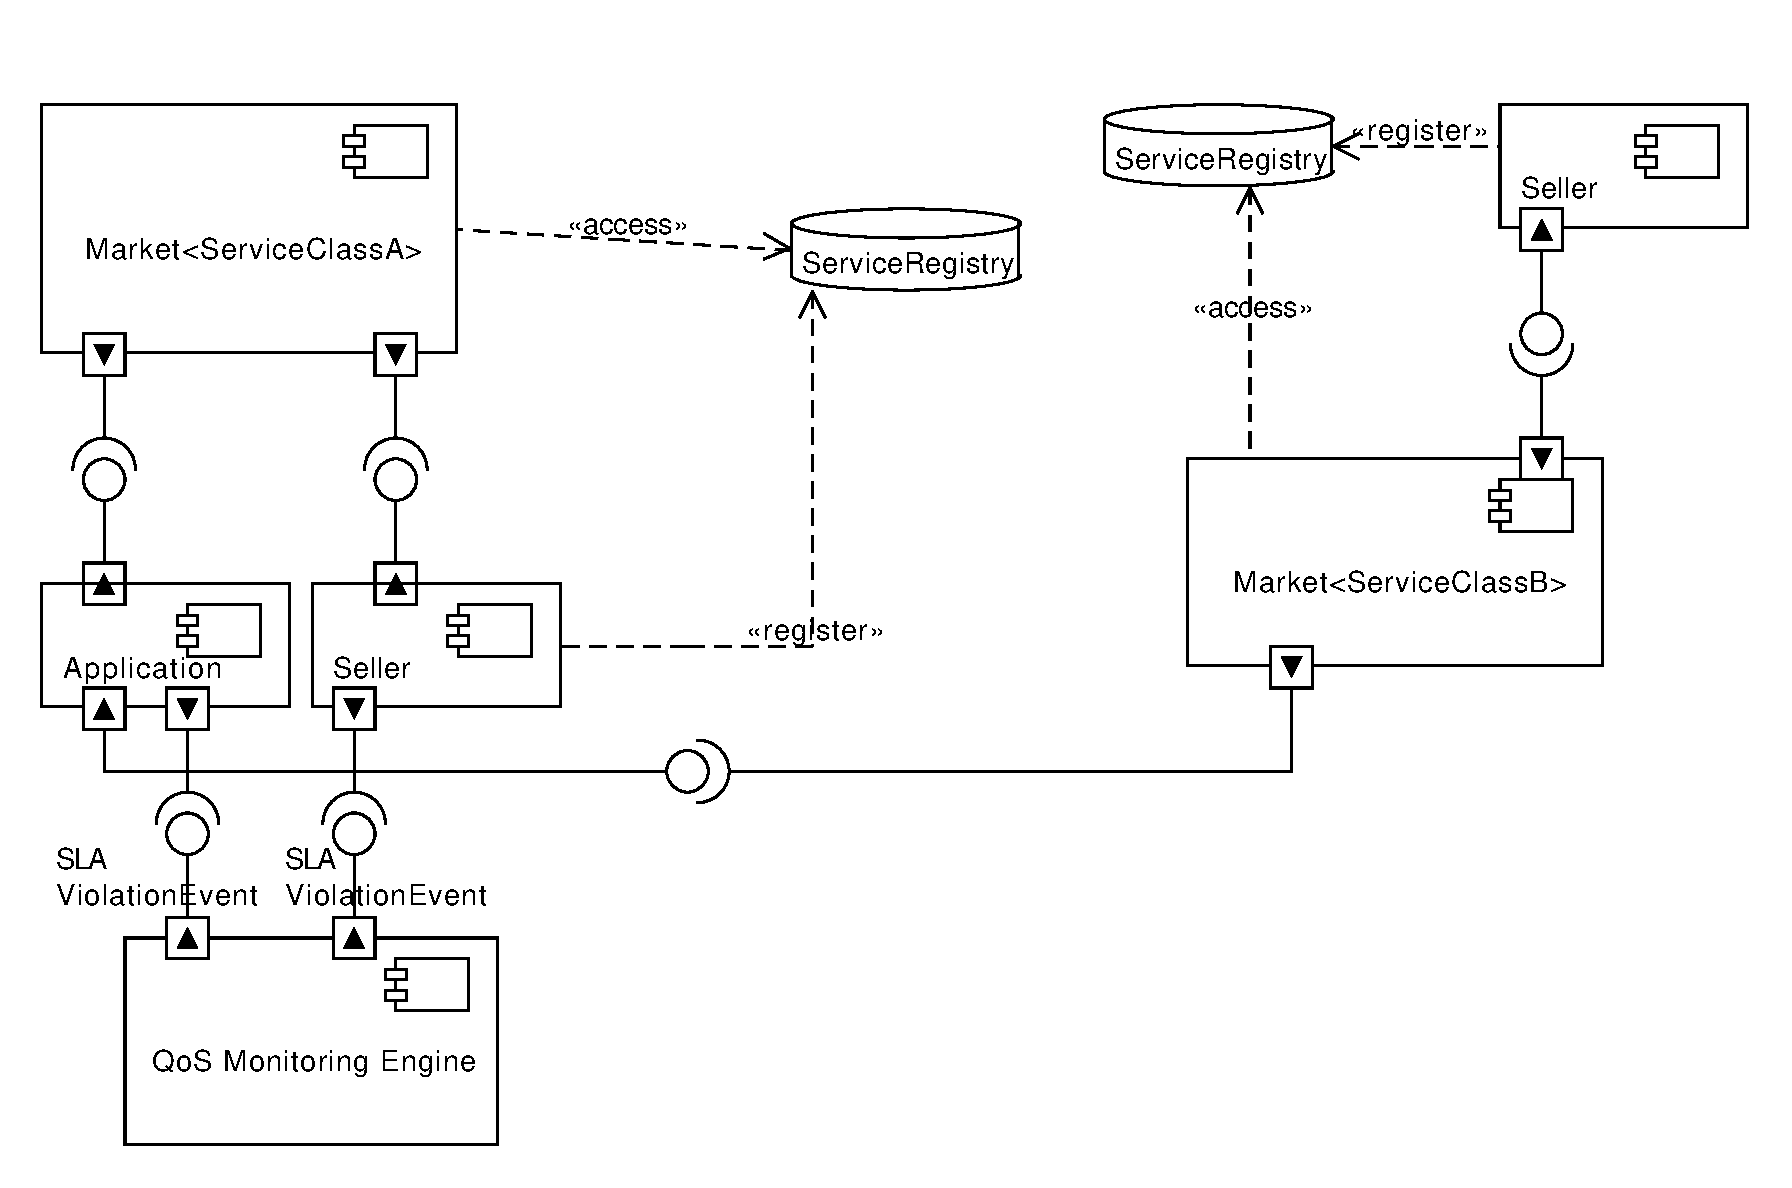
\includegraphics[scale=0.3]{drawings/Agent_Component_Diagram.pdf}
\caption{Component diagram of entities\label{fig:component_diagram}}
\end{figure}

\subsubsection{Class Diagram} The class diagram shows the static relationships between the main entities in the MAS. The \textit{Bid} and \textit{Ask} interfaces shown in figure \ref{fig:class_diagram} are also shown in the component diagram (see figure \ref{fig:component_diagram}), with the \textit{Market} class implementing both of them. 

\begin{figure}[H]
\centering
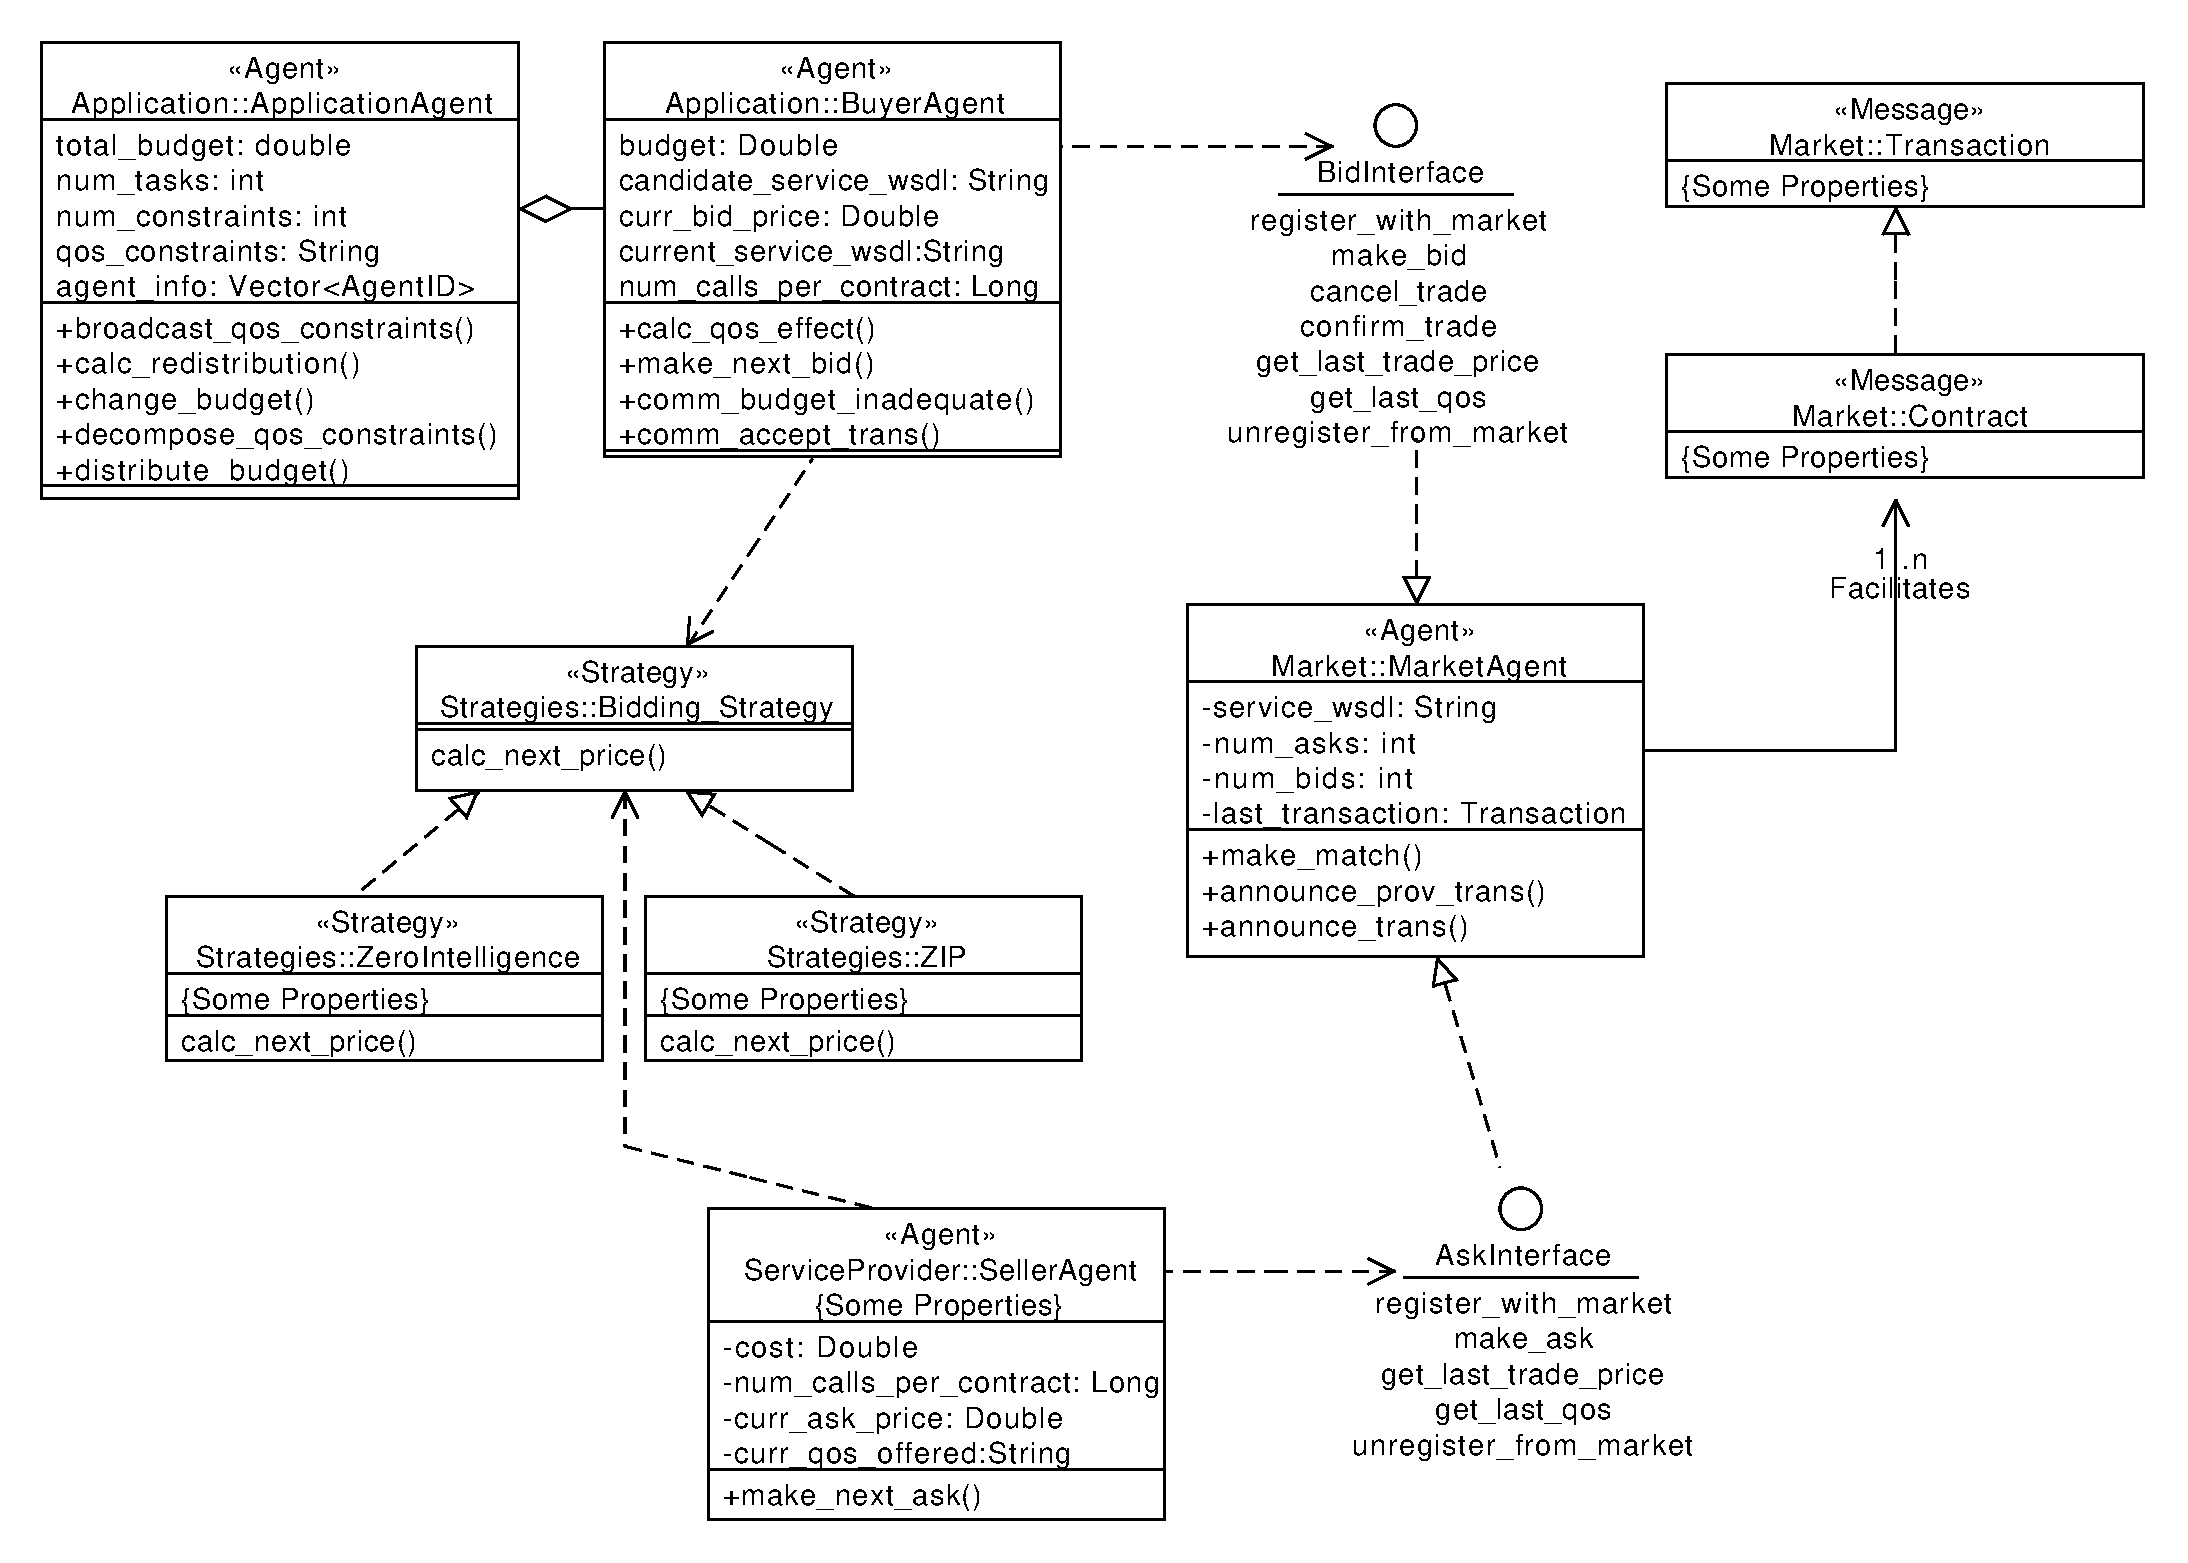
\includegraphics[scale=0.25]{drawings/Agent_Class_Diagram.pdf}
\caption{Class diagram of entities \label{fig:class_diagram}}
\end{figure}

\subsubsection{Activity Diagram} The most difficult part of getting all the agents in an MAS to solve a problem, is the problem of communication. The design of the communication protocol determines how much communication happens, at what times and how much computational effort it takes to communicate. If the agents communicate too little, then there is a danger of the MAS failing to solve the problem it was created for. On the other hand, if too much communication takes place, then a lot of wastage occurs, not only in terms of bandwidth but also in computational cycles and time. Thus, while communication is a fundamental activity in an MAS, depicting this in UML is difficult. The standard activity diagrams in UML are \textit{Sequence Diagrams} and \textit{Collaboration Diagrams}. However, the semantics in both these diagrams assumes a single thread of control, \textit{i.e.}, each object that sends or receives a message is assumed to be the only active object at that time instant. This is not true in the case of Clobmas.  Also, UML which does not provide for broadcast/multicast messages. To deal with these situations, the agent community has evolved AUML (Agent-UML) which modifies the semantics of a sequence diagram, to allow for the possibilities above. We document the communication steps of our mechanism through AUML diagrams.\\
In the following figures, we show the communication for an application with two AbstractServices, \texttt{A} and \texttt{B}, and its corresponding BuyerAgents and the market agent. The \emph{Setup Phase} (figure \ref{fig:setup_phase}) is composed of two calculations done by the ApplicationAgent and, two multicast messages to the application's BuyerAgents. The two calculations involve decomposing the application's end-to-end constraints into local constraints and, computing the budget that each BuyerAgent will receive.
\begin{figure}[h]
\centering
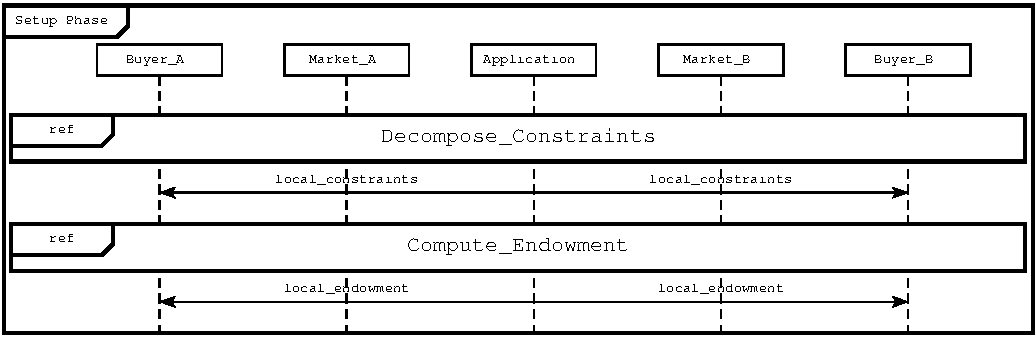
\includegraphics[scale=0.3]{drawings/setup_phase.pdf}
\caption{Setup phase for an application with two AbstractServices A \& B \label{fig:setup_phase}}
\end{figure}

Decomposing constraints (figure \ref{fig:decompose_constraints}) involves communication between the BuyerAgents, their respective markets and the ApplicationAgent. The ApplicationAgent waits for the BuyerAgents to get data about previous transactions in the market, applies SWR \cite{Cardoso2002Workflow} and checks whether the combination of QoS available in the market meets its end-to-end constraints. Based on the combinations that meet the end-to-end constraints, the ApplicationAgent creates local constraints for the individual BuyerAgents. These are then propagated to the BuyerAgents.
\begin{figure}[h]
\centering
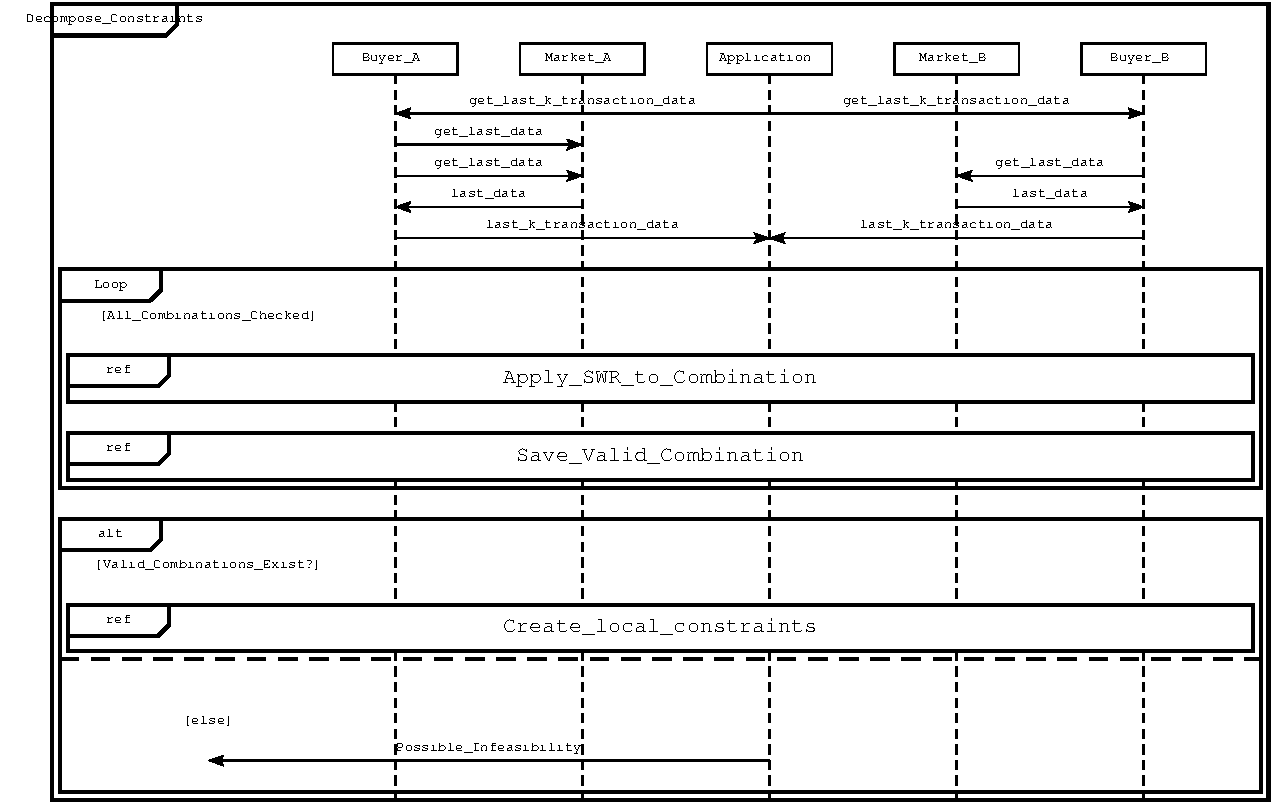
\includegraphics[scale=0.3]{drawings/decompose_constraints.pdf}
\caption{Application decomposes its constraints into local constraints \label{fig:decompose_constraints}}
\end{figure}

The budget for the individual agents is split in the ratio of the transaction prices that are prevalent in the individual markets. Given historical price information in a market, the prices in the next trading rounds are likely to be around the same figure. Splitting the application's budget evenly across the BuyerAgents could possibly result in some agents getting excess endowment, and some agents too less. The ratio of their transaction prices allows the agents with expensive services to get a naturally higher share of the budget.
\begin{figure}[h]
\centering
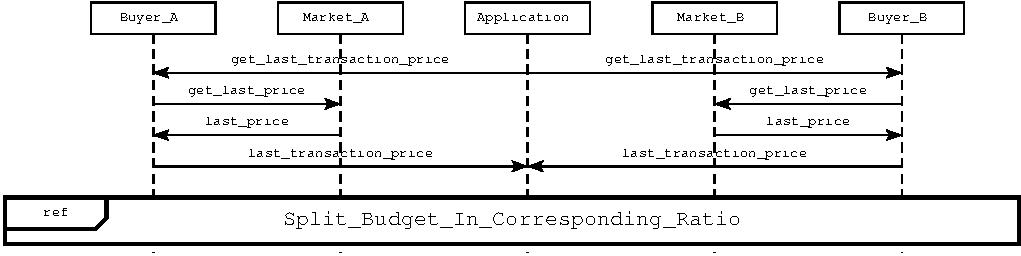
\includegraphics[scale=0.4]{drawings/compute_endowment.pdf}
\caption{Application computes endowment for its BuyerAgents}
\end{figure}

%\begin{figure}
%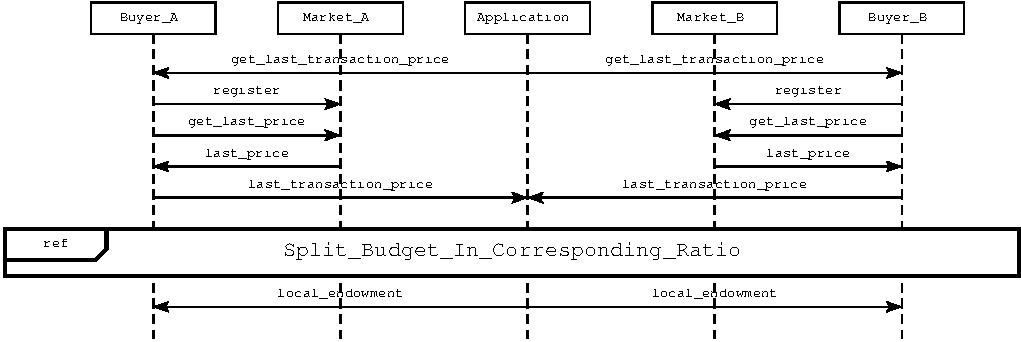
\includegraphics[scale=0.7]{figures/chapter4/distribute_budget.pdf}
%\end{figure}

In figure \ref{fig:trading_phase}, we show the communication that takes place during the trading phase. This phase is essentially a loop. It periodically evaluates the \textit{bids} and \textit{asks} in the orderbook, and tries to match them. If it is successful, the transaction moves into the second stage (see figure \ref{fig:cda_protocol}). Based on whether a trade occurs or not, the application evaluates whether it needs to re-distribute the endowments of its agents. It is possible that an agent is unable to find any potential transactions, simply because it does not have the budget to bid high enough.

\begin{figure}[h]
\centering
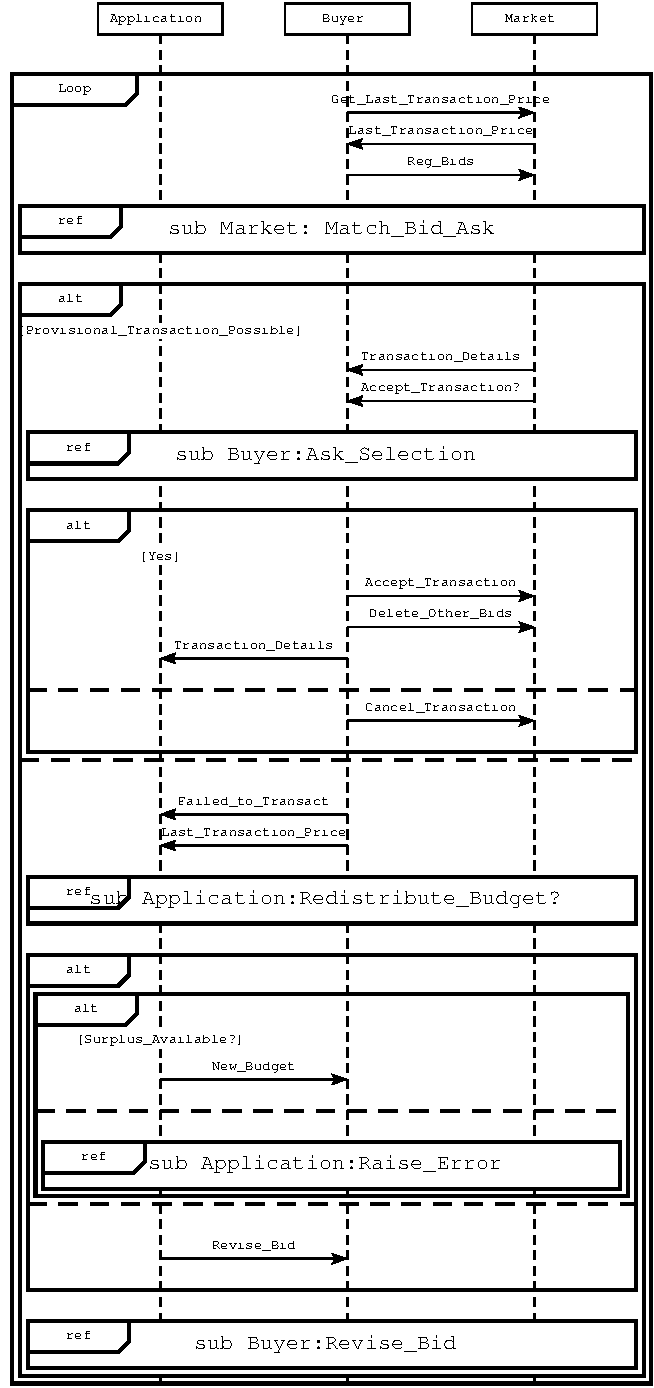
\includegraphics[scale=0.3]{drawings/trading_phase.pdf}
\caption{The trading phase of buying a service \label{fig:trading_phase}}
\end{figure}


The trading proceeds in two stages. In the first stage, the MarketAgent matches the bids and asks based on their individual QoS values and shout prices. After matching, a provisional transaction is created. This provisional transaction enters the second stage. In the second stage, the BuyerAgent compares all the Asks returned as provisional transactions (see section \ref{calculation_of_preference}). The top-ranked Ask is selected and the other Asks are rejected. The BuyerAgent enters into a transaction with the SellerAgent of the selected Ask.
\begin{figure}[h]
\centering
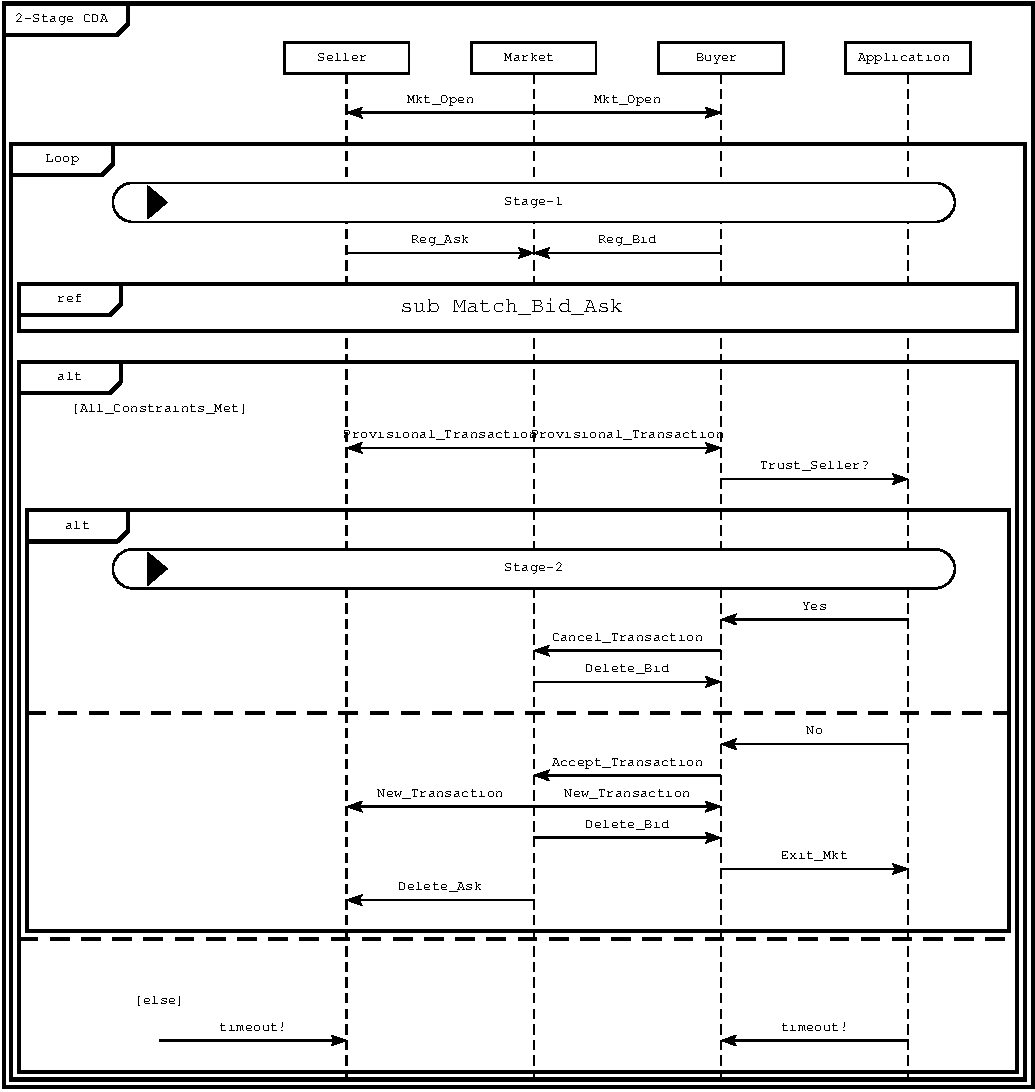
\includegraphics[scale=0.3]{drawings/cda_protocol.pdf}
\caption{Two-stage CDA protocol \label{fig:cda_protocol}}
\end{figure}

\subsubsection{Implementation of double auction} The most computationally intensive aspect of the entire system is the implementation of the double auction mechanism. Storing the bids and asks as simple lists results in a huge amount of searching for matching purposes. We modify the 4-heap data structure, as suggested in \cite{Wurman1998Flexible}, to store our multi-attribute bids and asks. In our python implementation, we use the heapq module to store bids in a descending order and asks in an ascending order. This decision allows for bids that are willing to pay a higher price, get matched first. 

\section{Evaluation}
\subsection{The Current Scenario}
The current form of service-selection is provider-driven. That is, in all commercial clouds, the cloud provider uses a \textbf{posted-offer} mechanism. A posted-offer is a form of market where the supplier posts a certain price on a \textit{take-it-or-leave-it} basis. Thus, on Amazon's \textit{elastic cloud compute} (EC2), there are several services that are functionally identical, but priced differently. This price differentiation exists due to different QoS being exhibited by these services.  In table \ref{tbl:amazon_prices}, we show a slice of Amazon's pricing for its \textit{On-Demand Instances}.
\begin{table*}\footnotesize
	\centering
	 \begin{tabular}{|p{5cm}|p{3cm}|p{3cm}|}
		\hline
		 \multicolumn{1}{|}{}& \multicolumn{1}{c}{Linux/UNIX usage} & \multicolumn{1}{c|}{Windows usage} \\ 
		 \multicolumn{1}{|c}{\textbf{Standard On-Demand Instances}} & & \\ \hline
			Small (default) & \$0.085 per hour & \$0.12 per hour \\ \hline
			Large & \$0.34 per hour & \$0.48 per hour \\ \hline
			Extra Large & \$0.68 per hour & \$0.96 per hour \\ \hline
			\multicolumn{1}{|c}{\textbf{Micro On-Demand Instances}} & & \\ \hline
			Micro & \$0.02 per hour & \$0.03 per hour \\ \hline
			\multicolumn{1}{|c}{\textbf{Hi-Memory On-Demand Instances}} & & \\ \hline
			Extra Large & \$0.50 per hour & \$0.62 per hour \\ \hline
			Double Extra Large & \$1.00 per hour & \$1.24 per hour \\ \hline
			Quadruple Extra Large & \$2.00 per hour & \$2.48 per hour \\ \hline
		\end{tabular}
	\caption{On-Demand Instance Pricing on Amazon EC2}
	\label{tbl:amazon_prices}
\end{table*}
Depending on the type of job envisioned, customers purchase a basket of computational power from Amazon. However, currently, there is no mechanism to automatically switch from one kind of \textit{On-Demand Instance} to another. Customers have to forecast the type of demand for their application in advance, and appropriately chose their package from Amazon. Any application that desires to use a particular service, has to pay the posted price. There exists no mechanism to negotiate/bargain with Amazon, on pricing or QoS of the services being offered. This has the very obvious effect of customers either over-provisioning or under-provisioning for their actual demand. If an application under-provisions, then it risks losing customers due to lack of QoS. On the other hand, if it over-provisions, it loses money due to lack of productive use. In both cases, the customer faces a loss.
\subsection{Empirical Study}
\textit{BizInt}, a small startup company creates a new business intelligence mining and visualization application.  It combines off-the-shelf clustering algorithms with its proprietary outlier detection and visualization algorithms, to present a unique view of a company's customer and competitor ecosystem. In order to exhibit a high level of performance, it decides to host its application in the cloud. Also, instead of reinventing the wheel, it uses third-party services (for clustering, etc.) that are also hosted in the same cloud. As seen in figure \ref{fig:BizIntWorkflow}, BizInt uses composite web services (Data Filtering, Clustering, Association Rule Mining and Cross-Validation) from the cloud, along with its own services (Job Submission, Outlier Detection and Visualization) to create a complete application.
\begin{figure}%
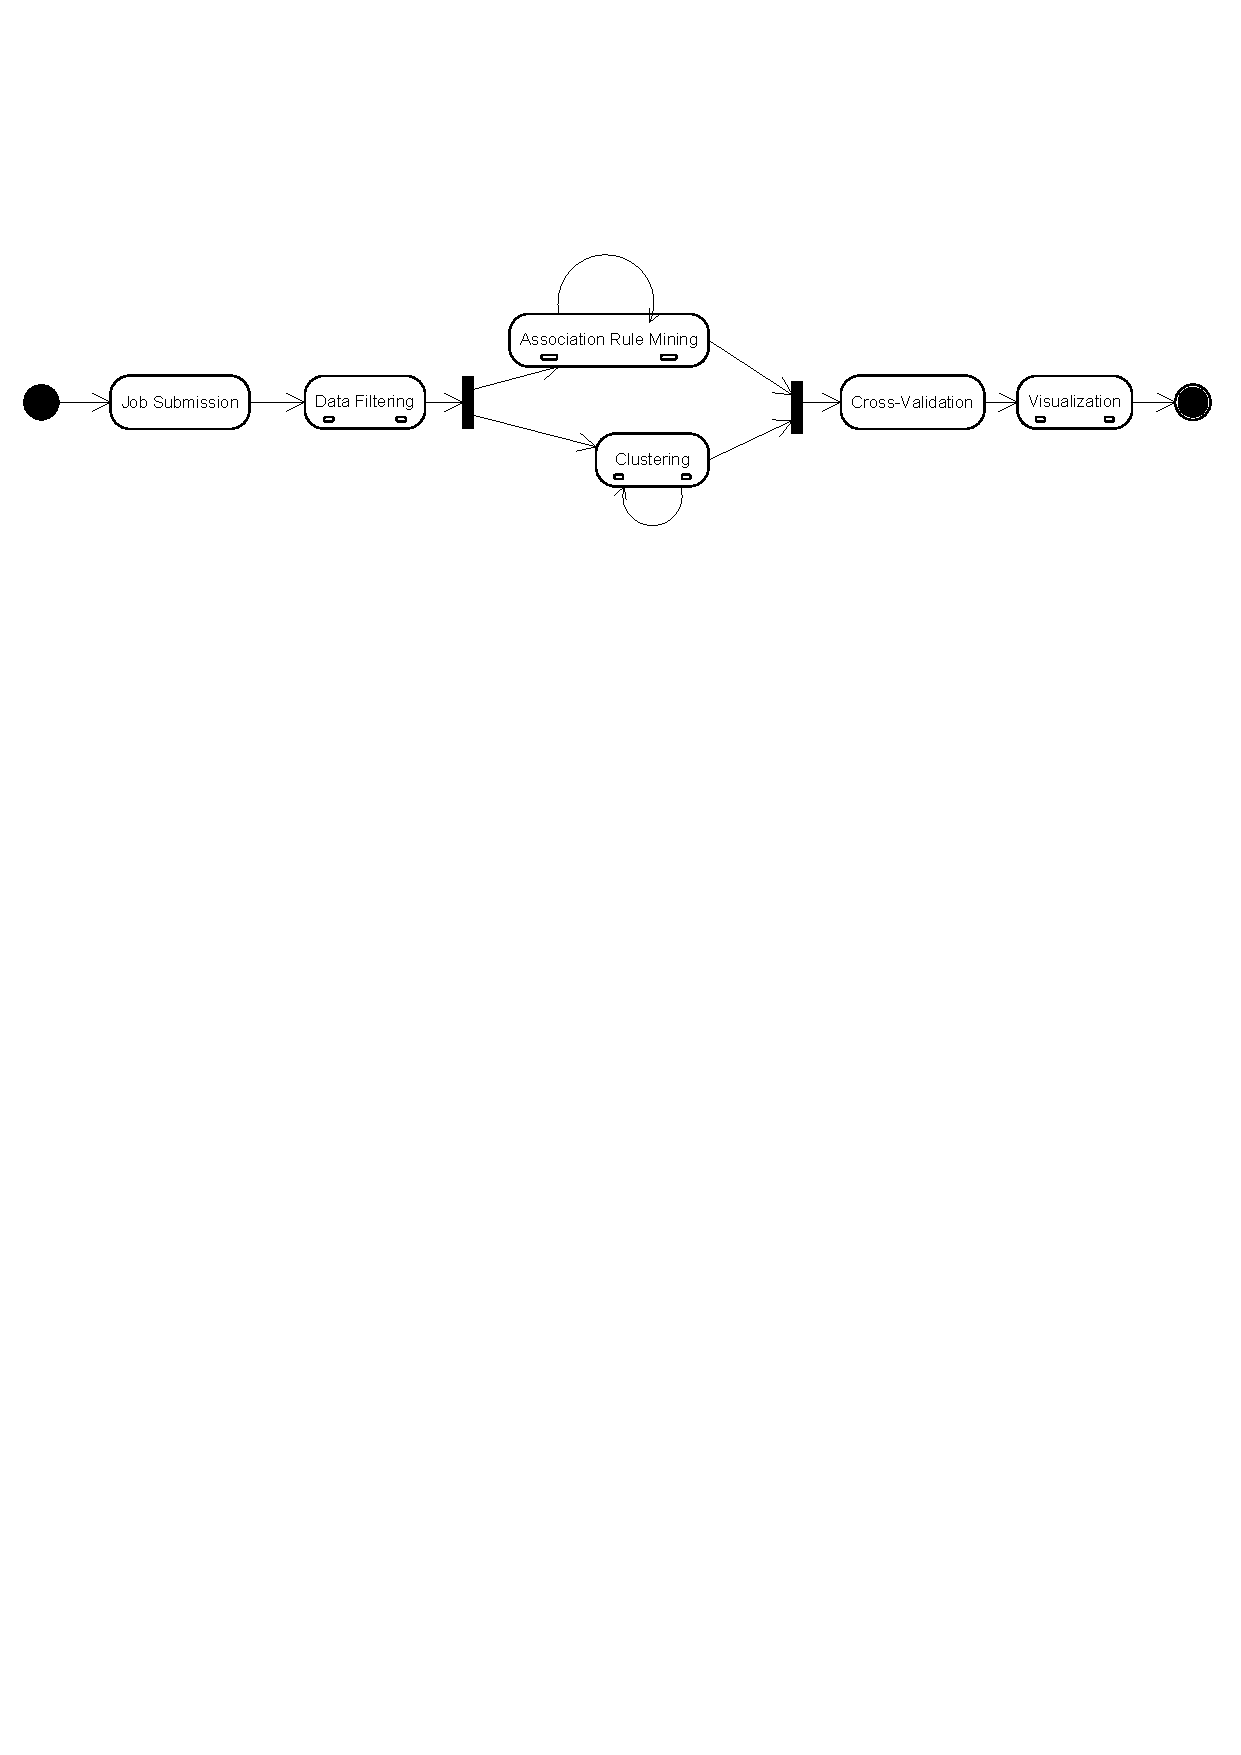
\includegraphics[scale=0.4, clip, trim=0 20cm 0 4cm]{drawings/BizIntWorkflow.pdf}%
\caption{BizInt's workflow constructed using composite services from the hosting cloud\label{fig:BizIntWorkflow}}%
\end{figure}
Soon BizInt discovers that different jobs emphasize different QoS. Some jobs want data to be processed as fast as possible, others require a high amount of security and reliability. In order to exhibit different QoS, BizInt needs to dynamically change its constituent services. \\
\textbf{SkyCompute} is a new entrant to the field of Cloud Computing. It wants to compete with Amazon, 3Tera, Google, Microsoft and other established cloud-providers. In order to attract cost and QoS-conscious customers, SkyCompute will have to differentiate its cloud from the others. It plans to target the \textit{Software-As-A-Service} market. Instead of providing specialist infrastructural services (like Amazon) or application framework services (like Google and Microsoft),it is planning to provide generically useful services like indexing, clustering, sorting, etc. Like most cloud providers, it plans to provide services with different QoS levels, so that multiple types of clients can be attracted to use it. To differentiate itself, SkyCompute plans to provide an adaptive framework, so that companies like BizInt can change their constituent services, dynamically.

\subsection{Qualitative Criteria}
Thus, \textit{clobmas} must fulfill the following criteria:
\begin{enumerate}
		\item Allows customers like BizInt to create adaptive applications
		\item Generates a higher utilization of services than the posted-offer model currently followed (for SkyCompute)
	\end{enumerate}

\subsection{Quantitative Criteria}
Since, SkyCompute is an ultra-large collection of services, clobmas must be able to scale to large numbers of applications and ConcreteServices. Since there is no public data about the kinds of workflows hosted on commercial clouds, and their corresponding service choices, we made assumptions about the variables involved in dynamic service composition. We make these assumptions based on conversations with performance consultants at Capacitas Inc., and numbers gleaned from the literature review.
       	  
%    \paragraph{Scaling Goals}
%	    \begin{enumerate}
%	        \item Ratio of increase in AdaptationTime to increase in CandidateServices increases linearly or as a low-order polynomial
%			\item Ratio of increase in AdaptationTime to increase in markets increases linearly or as a low-order polynomial
%			\item Number of applications that have adapted in all cases shall not be lower than 70\% of the market 
%	    \end{enumerate}
We summarize the operational ranges that clobmas is expected to deal with, in table \ref{tbl:scalability_targets}
\begin{table*}[h]
\centering
\renewcommand{\arraystretch}{1.5}
\begin{tabular}{p{10cm}p{4cm}p{3cm}}
	\toprule
	\textbf{Variable affecting performance} & \textbf{From Lit. Review} & \textbf{Target Goals}\\ 
	\midrule
	Number of AbstractServices in a workflow & \hspace{1.8cm} 10 & \hspace{1.5cm} 20 \\ 
	CandidateServices per AbstractService & \hspace{1.8cm} 20 & \hspace{1.5cm} 50 \\ 
	QoS attributes considered per CandidateService & \hspace{1.8cm} 3 & \hspace{1.5cm} 10 \\ 
	Number of markets considered per CandidateService & \hspace{1.8cm} 1 & \hspace{1.5cm} 10 \\ 
	\bottomrule
\end{tabular}
\caption{Operational range for scalability goals \label{tbl:scalability_targets}}
\end{table*}

\subsection{Experimental Setup}
Although open-source cloud implementations like OpenNebula\footnote{www.opennebula.org}, and Eucalyptus\footnote{http://www.eucalyptus.com/} are freely available for download, they are primarily targetted at the \textit{Infrastructure-As-A-Service} market. Also, modifying these implementations for our purposes (to introduce the notion of markets), would be cumbersome and expensive. In the same vein, using simulators such as CloudSim would require major modifications, to those toolkits. CloudSim is a fairly new toolkit, and does not have the ability to explore market mechanisms in a sophisticated manner\cite{Breskovic2011Towards}. 
\paragraph{Software}
In this scenario, we wrote our own simulator in Python (v. 2.6.5), using a discrete-event simulation library, SimPy\footnote{http://simpy.sourceforge.net/}. The operating system in use, was 64-bit Scientific Linux.
\paragraph{Hardware}
All experiments were run on an Intel Dual-cpu Quad-Core 1.5Ghz workstation, with 4MB of level-1 cache and 2GB of RAM.
\subsection{Methodology}
We simulate 300 applications, each application consisting of randomly generated workflows trying to achieve their desired QoS levels, within a given budget. The budget that each application gets, acts as a constraint and the application's constituent BuyerAgents can never bid above their budgets. Each application generates a random level of QoS that it must achieve. Once an application achieves its required QoS, it withdraws from trading until an internal or external stimulus occurs. We model the probability of a QoS service violation based on a study by Cloud Harmony\cite{2011CloudHarmonyStudy}.\\
%An external stimulus occurs when the application decides to change its required QoS for any reason (say, a new job requires different QoS levels). This is simulated by using time as a parameter. Every application, once satisfied with its QoS, (as mentioned above) stops adapting. However, at some random time, every application receives a different job that requires different QoS levels. This prompts that particular application to adapt, and therefore, approach the market again.
 %, based on a study conducted by Cloud Harmony \cite{2011CloudHarmonyStudy}
% \subsection{Scalability}
% The scalability of a self-adaptive approach is slightly difficult to measure, since we're concerned not only with time and space complexity, but also with goodness complexity. 


\subsection{Results}
There are two perspectives from which to evaluate our mechanism, BizInt's and SkyCompute's perspective. We present both perspectives, with an emphasis on SkyCompute's view since it provides a better idea on the scalability of our mechanism. All simulations are reported as an average of a 100 simulations.\\
\subsubsection{BizInt's Perspective}
From BizInt's perspective, a cloud provider that enabled applications to self-adapt at the QoS level would be ideal. BizInt understands that a typical adaptation process does not guarantee an optimal result. But, even so, a self-adaptive mechanism would be a step-up from the current mechanism of manually selecting the service to be used. It evaluates the efficacy of the adaptive mechanism by two measures:
	\begin{enumerate}
		\item How close to the desired QoS level does the adaptive mechanism reach?
		\item How long does it take for an application to achieve its desired QoS?
	\end{enumerate}
\paragraph{Close to desired QoS}  We use the application's targetted end-to-end QoS as the benchmark, against which the currently achieved QoS is measured. The application's target QoS is normalized and summed across all the QoS that it is interested in. This is taken to be the \textit{ideal utility level}. The achieved QoS is fed through the same process, to attain the \textit{achieved utility level}. The difference between the \textit{ideal utility level} and \textit{achieved utility level} is called the \textit{quality gap}. Each application defines a tolerance level, that specifies the magnitude of quality gap that is acceptable. \textbf{If the quality gap is within the tolerance level, the application is said to be satisfied}. We measure over a trading period, the \textbf{number of rounds that the application is satisfied}.

\paragraph{Time to Satisfaction} In the absence of a deterministic solution (and therefore a deterministic notion of time), we must contend ourselves with evaluating whether the adaptive algorithm is \textit{`fast-enough'}.  The natural unit of time in clobmas, is a \textit{trading round}.  We measure \textbf{how many trading rounds}, application takes to be satisfied, from the start of an adaptation event. An adaptation event occurs when an application notices that the \textit{quality gap} is beyond the tolerance level. Thus, the start of the simulation defines an adaptation event, since all applications start off without any \textit{achieved utility level}.
	
In figure \ref{fig:goodness} we see an average application's achievement of QoS levels. The application starts off with a \textit{quality gap} of \textit{minus 3}, but it quickly adapts to the QoS demanded and reaches the tolerance zone, in about $20$ trading rounds. From this point on, the application stays satisfied. The application is satisfied for $280$ out of $300$ trading rounds. We see that the achieved utility level does not stay constant. Instead, internal adaptation events cause the application to seek out different services. However, it stays within the tolerance zone. In figure \ref{fig:goodness_cda}, we show the adaptation occurring  under conditions of normal distribution of QoS demand and supply in the cloud. 
 \begin{figure}[h]
 	\centering
    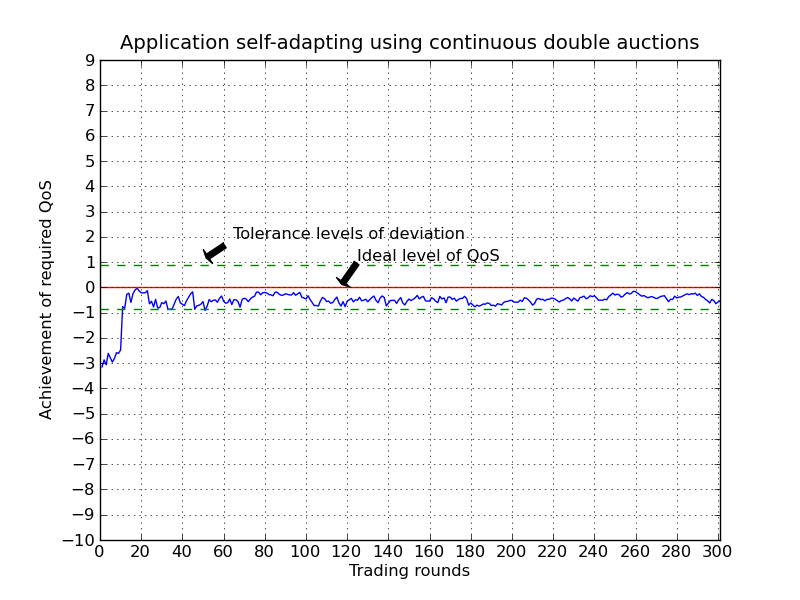
\includegraphics[scale=0.45]{graphs/Single_App_Self_Adaptation_Across_Rounds_With_QA_Change.png}
    \caption{Utility gained by adaptation by a single application \label{fig:goodness_cda}}
\end{figure}	 

To compare the goodness of trading in a CDA market, we contrast its use in a posted-offer market.
\paragraph{Posted Offer:} This type of mechanism refers to a situation where a seller posts an offer of a certain good at a certain price, but does not negotiate on either. That is, the buyer is free to \textit{take-it-or-leave-it}.  In such a scenario, the probability that an application will find services, at the \textit{bid-price} decreases. 

\begin{figure}[h]
	\centering
	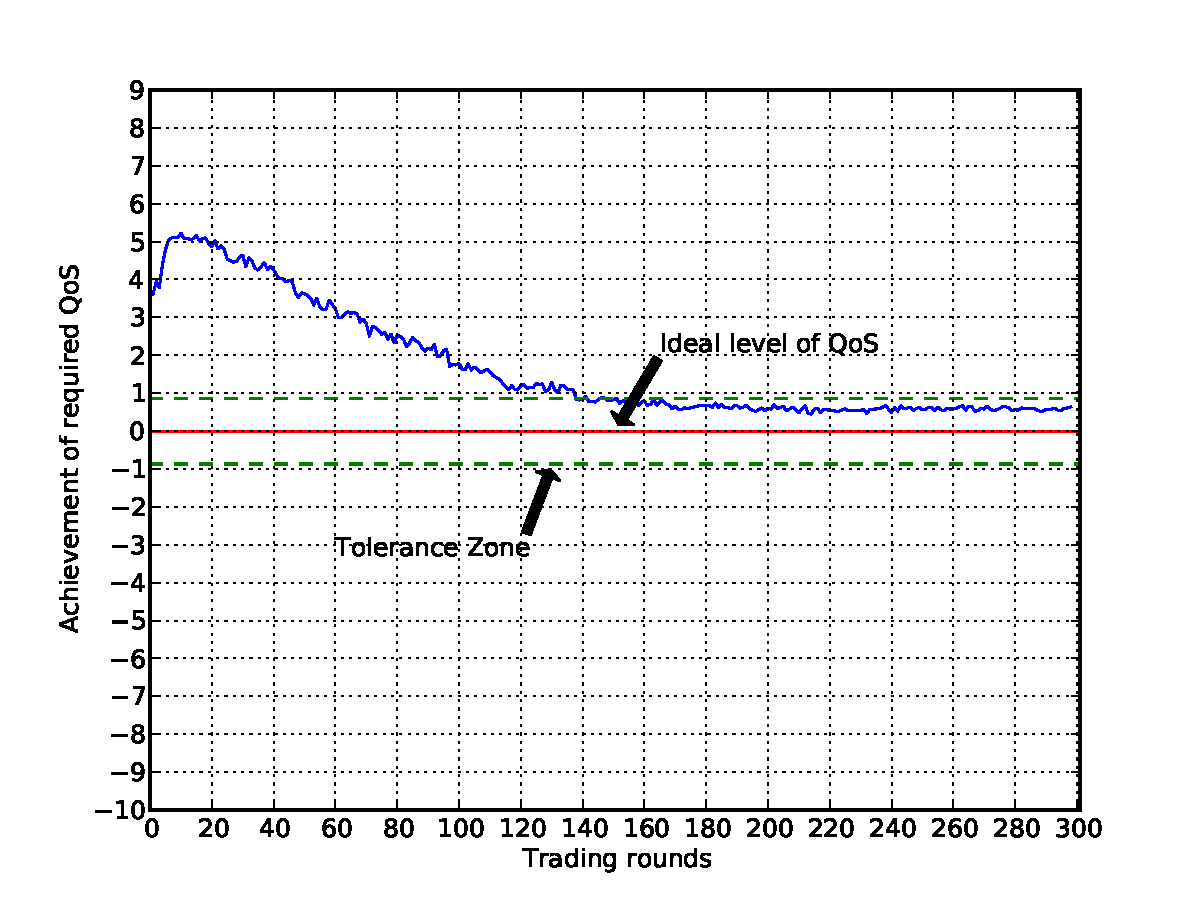
\includegraphics[scale=0.45]{graphs/posted_offer_singleapp_bimodal_qa.pdf}
	\caption{Utility gained by a single application in a posted offer market \label{fig:goodness_posted_offer}}
\end{figure}

In figure \ref{fig:goodness_posted_offer}, we see that the application is able to adapt and acquire the QoS that it requires. However, it is obvious from comparing the two figures, that in figure \ref{fig:goodness_cda}, the application is able to reach the tolerance zone a lot quicker than the application in figure \ref{fig:goodness_posted_offer}. In fact, in the \textit{posted offer} market, we see that the application takes $140$ rounds to reach the tolerance zone, while in the \textit{CDA} market, the application is able to reach its tolerance zone in under 20 rounds of trading. This difference can be attributed to the fact that since the sellers in a \textit{posted-offer} market do not change their price, the buying agents have to search a lot longer to find sellers that they are able to trade with. In a \textit{CDA}, the search process is much faster, since both the buyers and the sellers adjust their \textit{Bids} and \textit{Asks}.

\begin{table}[H]\footnotesize
\centering
\begin{tabular}{p{5cm}p{2cm}p{2cm}}
 \toprule
	& \textbf{CDA} & \textbf{PostedOffer} \\
 \midrule
	Number of rounds satisfied & 282 & 160 \\ 
	Time to reach QoS & 18 & 140 \\ 
\bottomrule
\end{tabular}
\caption{Comparative performance of adaptation in CDA vis-a-vis Posted Offer \label{tbl:comparative_performance}}
\end{table}
	
\subsubsection{SkyCompute's Perspective}	
SkyCompute would like to ensure that any mechanism that it offers for self-adaptation results in high utilization of its services. We define \textbf{market satisfaction rate} as a measure of the efficiency of the mechanism. \textbf{Market satisfaction rate} is the percentage of applications that are satisfied with their QoS achievement. A satisfied application would withdraw from trading and use the service for a relatively long period of time. The more the number of applications that are satisfied, the more the number of services from SkyCompute that are being utilized. Thus, \textbf{market satisfaction rate} is a measure that SkyCompute would like to maximize.\\
As a baseline, we first implement the Zero-Intelligence mechanism, as this represents the lower limit of the effectiveness of the CDA mechanism. The Zero-Intelligence scheme consists of agents randomly making bids and asks, with no history or learning or feedback(see figure \ref{fig:pure_random_strategy}). As expected, it performs quite poorly, with a market satisfaction rate of about 10-20\%. Clobmas achieves a much higher rate of market satisfaction(see figure \ref{fig:cda_zip_market_satisfaction}). 

\begin{figure}[h]
	\centering
    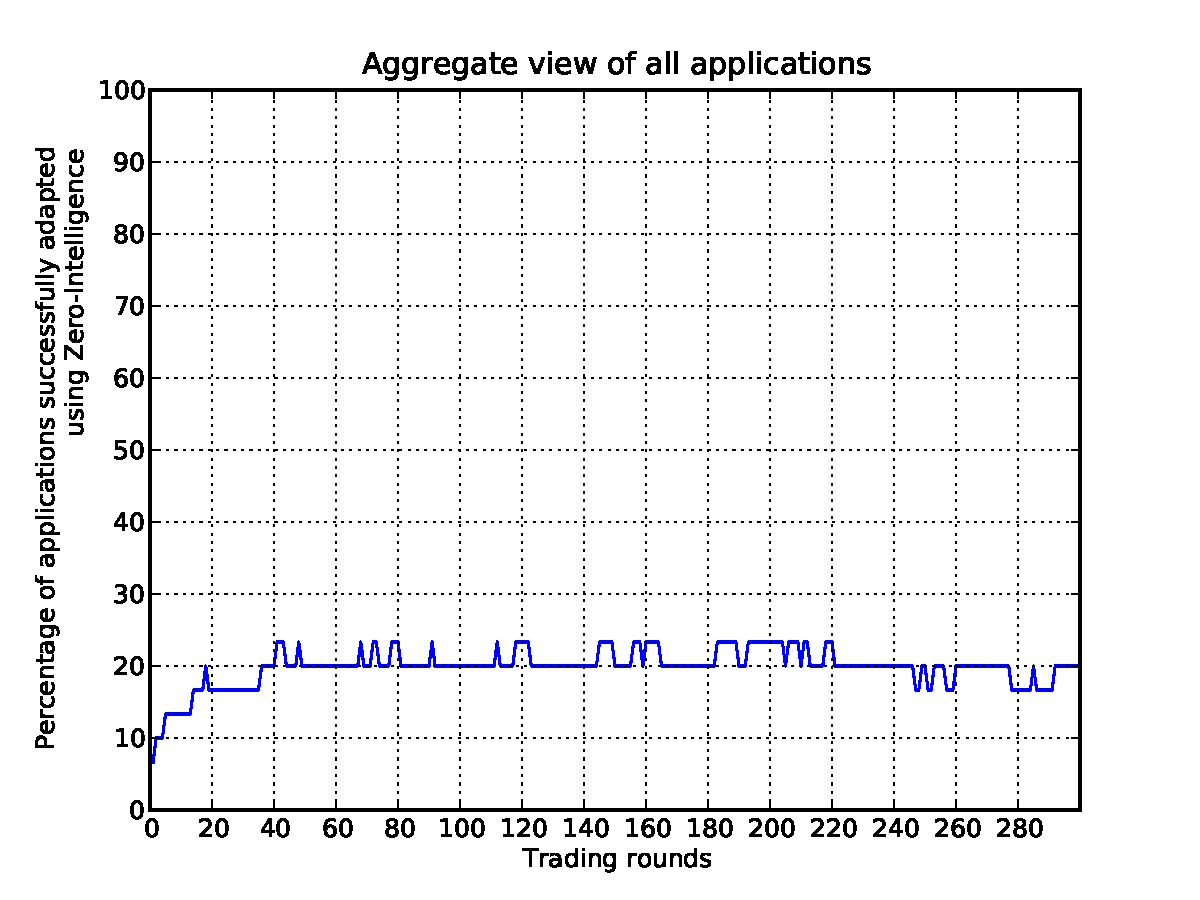
\includegraphics[scale=0.45, clip, trim=0cm 1cm 1cm 0.8cm]{graphs/efficiency-of-zi.pdf}
    \caption{Efficiency of adaptation in a CDA market with \textit{Zero Intelligence}\label{fig:cda_zi_market_satisfaction}}
\end{figure}

On the other hand, we see (in figure \ref{fig:cda_zip_market_satisfaction}) that with adaptive bids, the number of applications that are able to adapt rise to about 85\% of the total market. This is a huge improvement with a very small improvement in the intelligence of the agents.
\begin{figure}[h]
	\centering
	 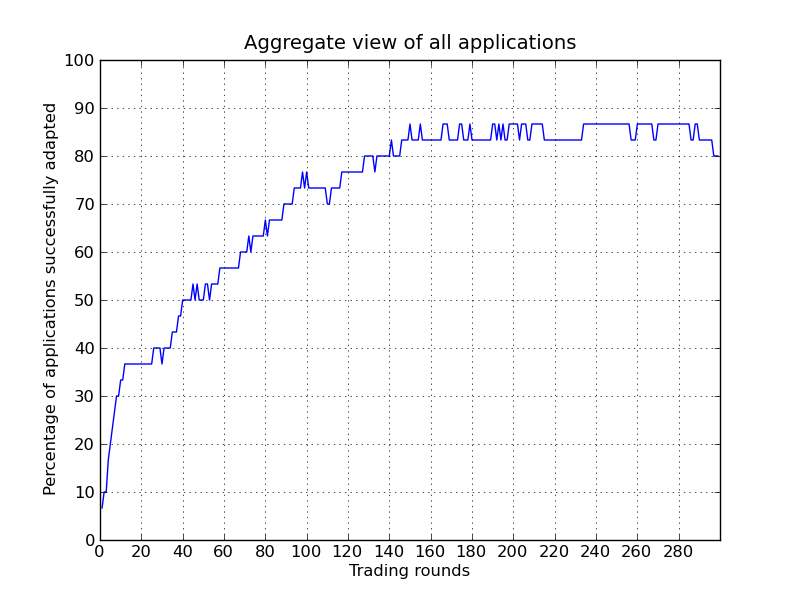
\includegraphics[scale=0.45, clip, trim=0cm 1cm 2cm 0.8cm]{graphs/probabilistic-change-to-qa.png}
	 \caption{Efficiency of adaptation in a CDA market \label{fig:cda_zip_market_satisfaction}}
\end{figure} 

Quite similar to the CDA, the posted-offer also performs well (approx 70\% market satisfaction rate). In this case, the sellers \textit{never} adjust their prices, but the buyers do. 

\begin{figure}[h]
	\centering
	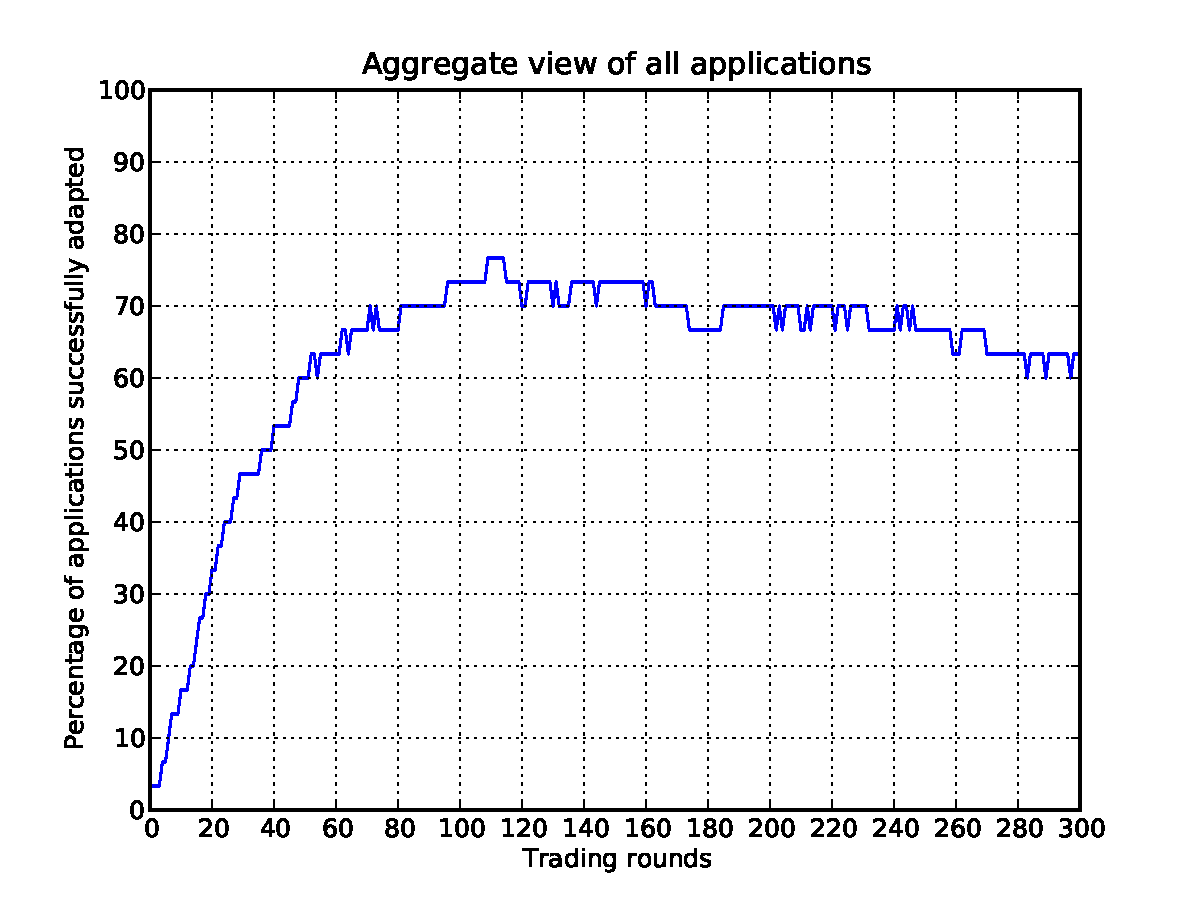
\includegraphics[scale=0.45]{graphs/posted_offer_2_cand_3_qa.pdf}
	\caption{Efficiency of adaptation in a Posted Offer market \label{fig:posted_offer_market_satisfaction}}
\end{figure}

%\paragraph{Market Conditions}
%Investigating the effect of market conditions (distributions of demand and supply) on the self-adaptive mechanism is slightly tricky. Conditions like paucity of supply, merely has the effect of less applications being able to satisfy their QoS requirements. The conditions that we investigate are shown in Table \ref{MarketConditions}. As can be seen from the table, the changing of QoS attribute demand and/or supply, from a uniform distribution to a skewed (bimodal) distribution does not seem to adversely affect the performance, at the aggregate level. More investigation, however, is required to establish the limits at which the aggregate performance starts to degrade noticeably.
%
%\begin{table*}[ht]
% \begin{tabular}{| c | l | l |}
% \hline
% & \small Uniform Distribution of QoS in Sellers & \small Skewed Distribution of QoS in Sellers\\ \hline
% \small Uniform Dist of QoS in Buyers & 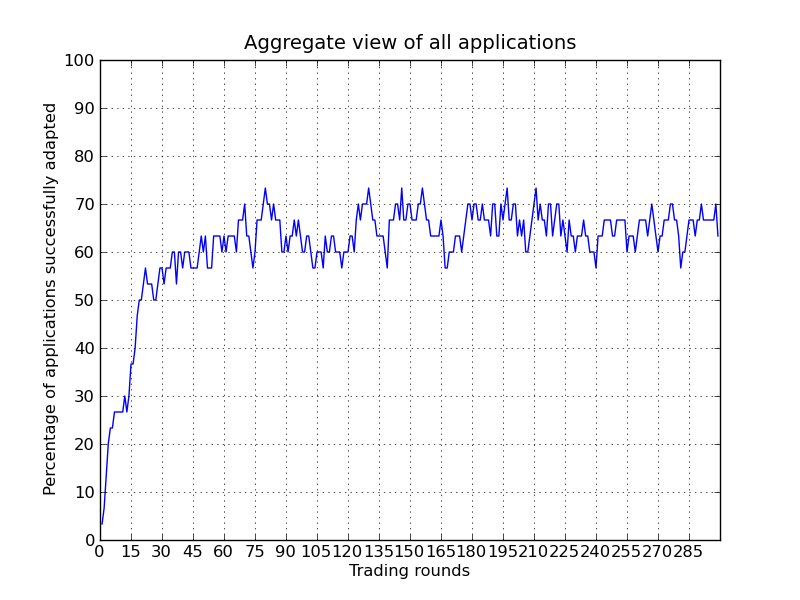
\includegraphics[scale=0.34] {graphs/uniform-seller-uniform-buyer.png} & 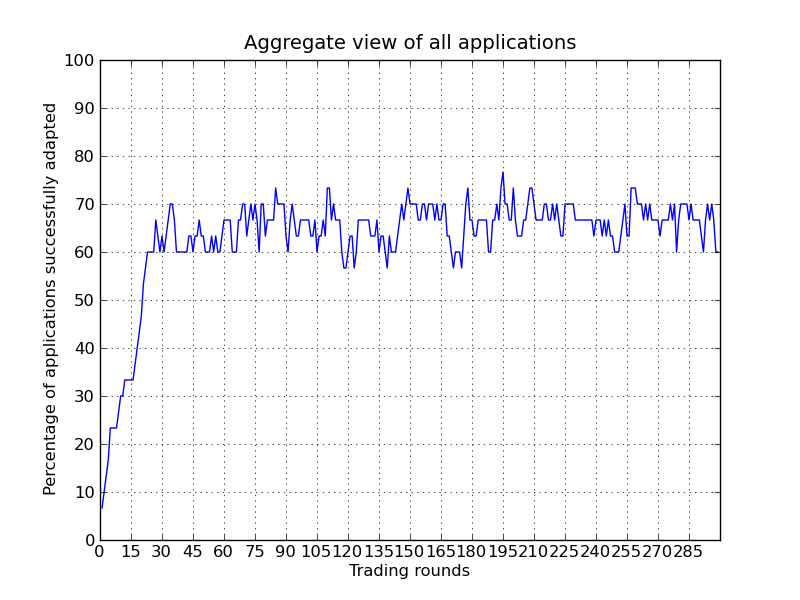
\includegraphics[scale=0.34] {graphs/uniform-seller-skewed-buyer.png}\\ \hline
% \small Skewed Dist of QoS in Buyers & 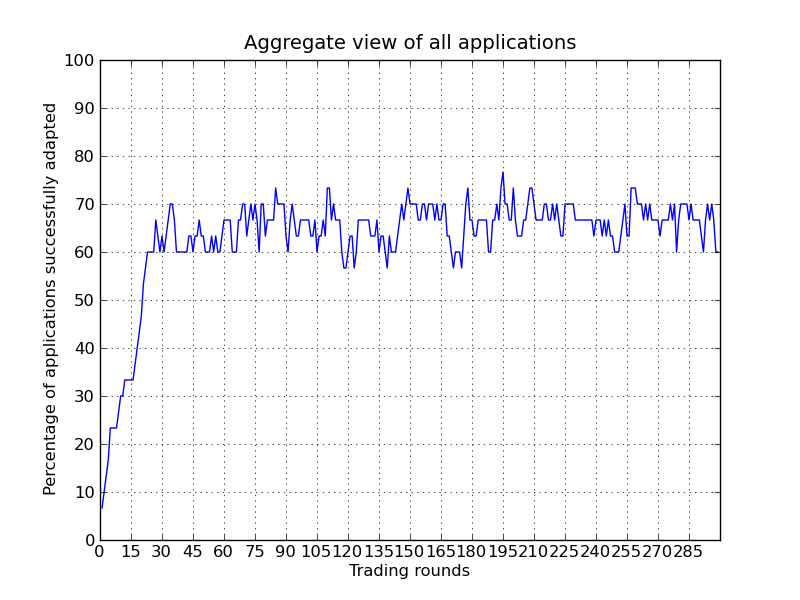
\includegraphics[scale=0.34] {graphs/uniform-seller-skewed-buyer.png} & 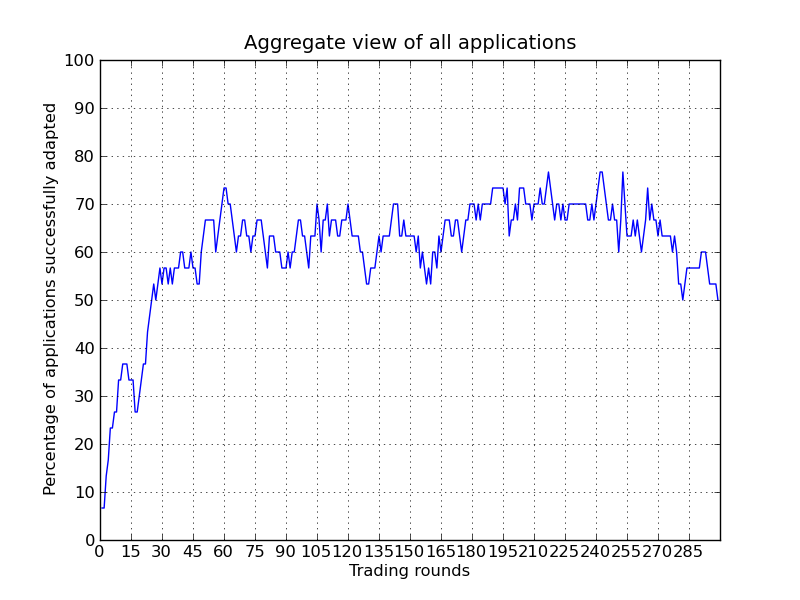
\includegraphics[scale=0.34] {graphs/skewed-seller-skewed-buyer.png} \\ \hline 
% \end{tabular}
% \caption[MarketConditions]{Depending on the kind of market conditions prevalent, applications find it easier/difficult to reach their target QoS levels. Predictably, we observe more fluctuation in the case of skewed supply and demand of QoS. Importantly though, in all four conditions, the macro behaviour of the system remains the same.} 
% \label{MarketConditions}
% \end{table*}
       
\subsection{Scalability Requirements for SkyCompute}
Although clobmas using a double-auction is better than clobmas using a posted offer, SkyCompute would like to know if this mechanism scales well. To investigate this, we pick a level of market satisfaction rate, that is higher than posted-offer, and measure how long it takes to achieve this level. The adaptation process can be highly dependent on many variables. In this section, we tease out how each of these variables affect the time taken for adaptation. To this end, we present the time taken by the CDA market to achieve an \textbf{80\%  market satisfaction rate}, while varying each of these variables.

\textbf{AbstractServices Vs. CandidateServices:}
Arguably, these are the variables that change most often from application to application, and from time to time. Every application has a different workflow and therefore, a different number of AbstractServices. As time passes, applications that have met their QoS will retire from the market, and new applications will come in. This changes the orderbook from the demand side. Also, the number of CandidateServices available per AbstractService is most susceptible to change. As time passes, some CandidateServices will no longer be available, and new ones come into the market. This changes the orderbook from the supply side.

\begin{figure}[htbp]
	\begin{minipage}[b]{0.4\linewidth}
	\hspace{0.5cm}
	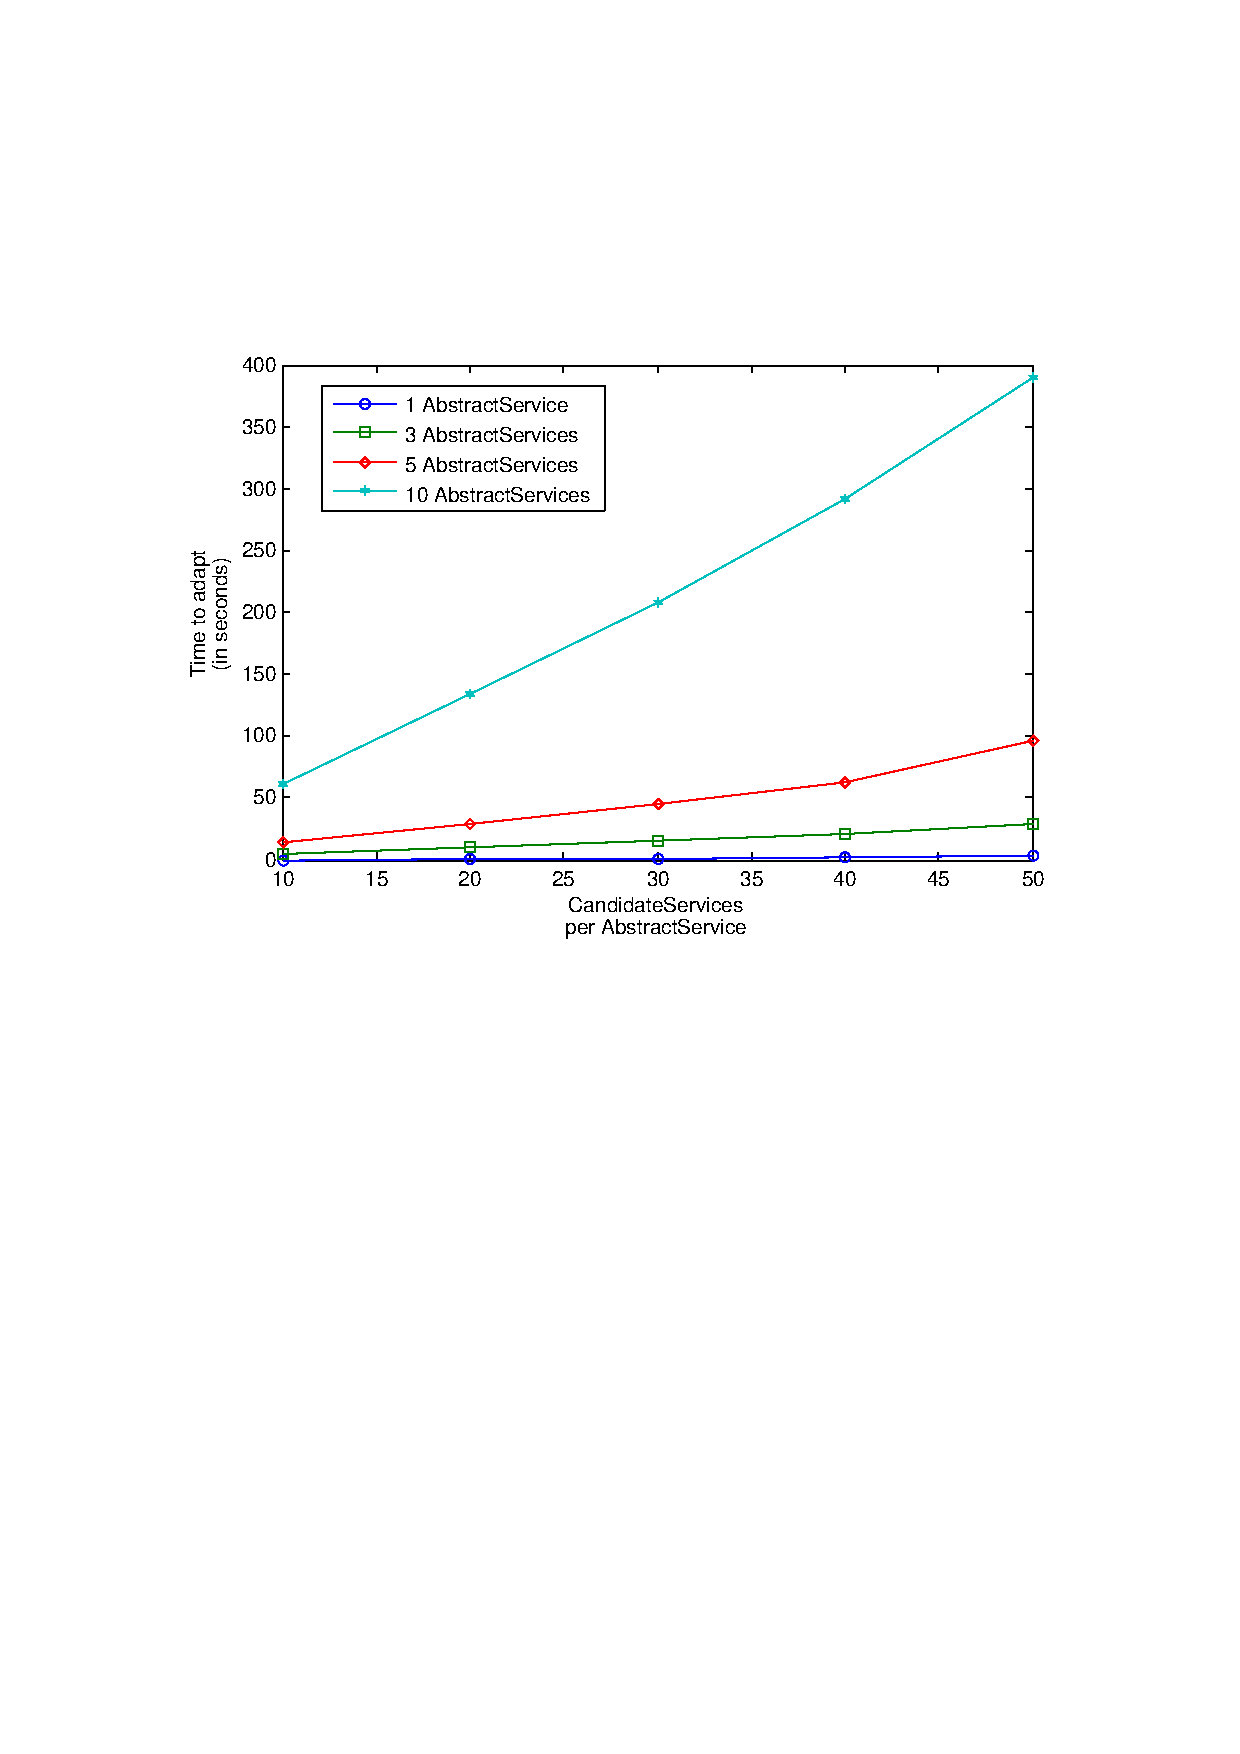
\includegraphics[clip, trim=5cm 14cm 2cm 6cm, scale=0.3]{graphs/1_3_5_10_task_per_svc_scaling.pdf}
	\caption{CandidateServices per AbstractService increase \label{fig:task_per_svc}}
	\end{minipage}
	\hspace{0.7cm}
	\begin{minipage}[b]{0.4\linewidth}
			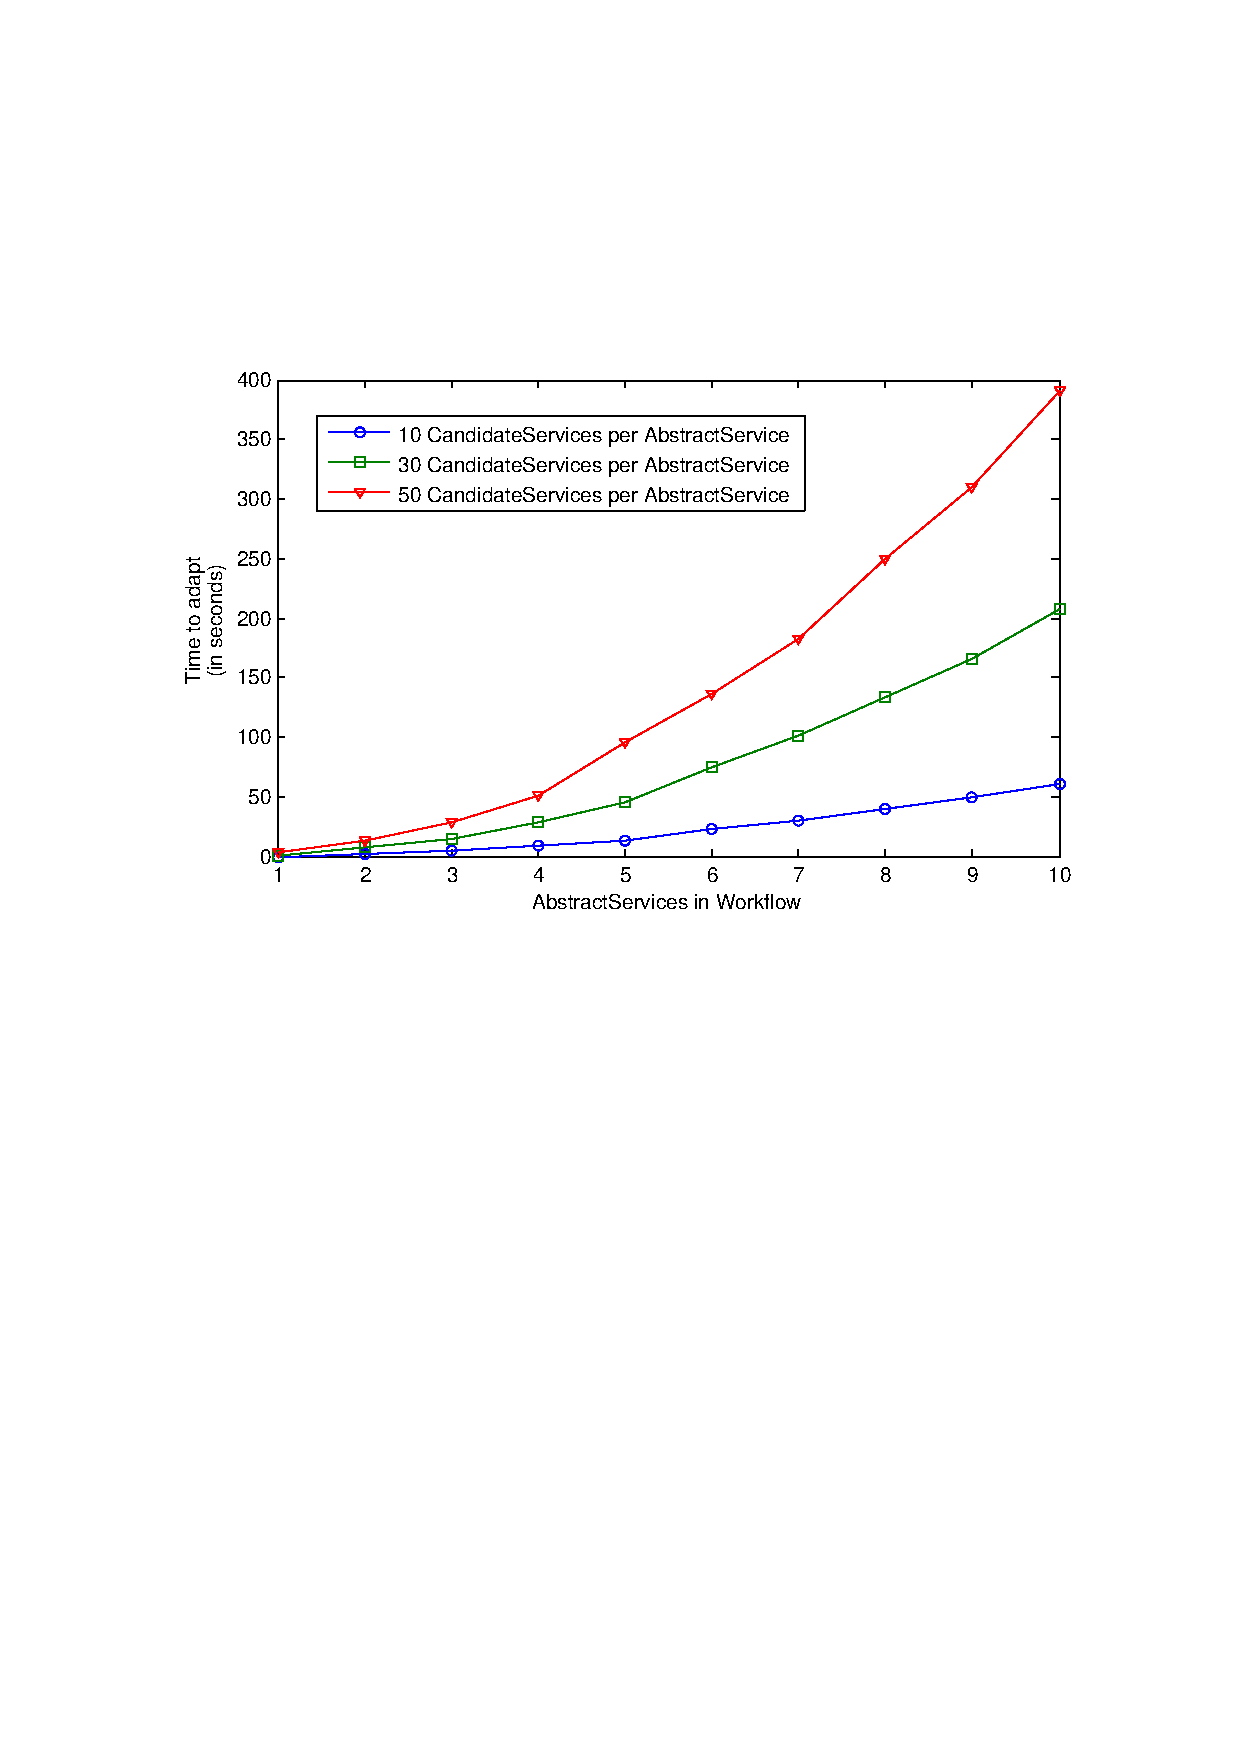
\includegraphics[clip, trim=2cm 14cm 2cm 6cm, scale=0.3]{graphs/10_30_50_svc_per_task_scaling.pdf}
			\caption{AbstractServices in workflow increase\label{fig:svc_per_task}}
	\end{minipage}
\end{figure}

\begin{figure}[htbp]
	\centering
	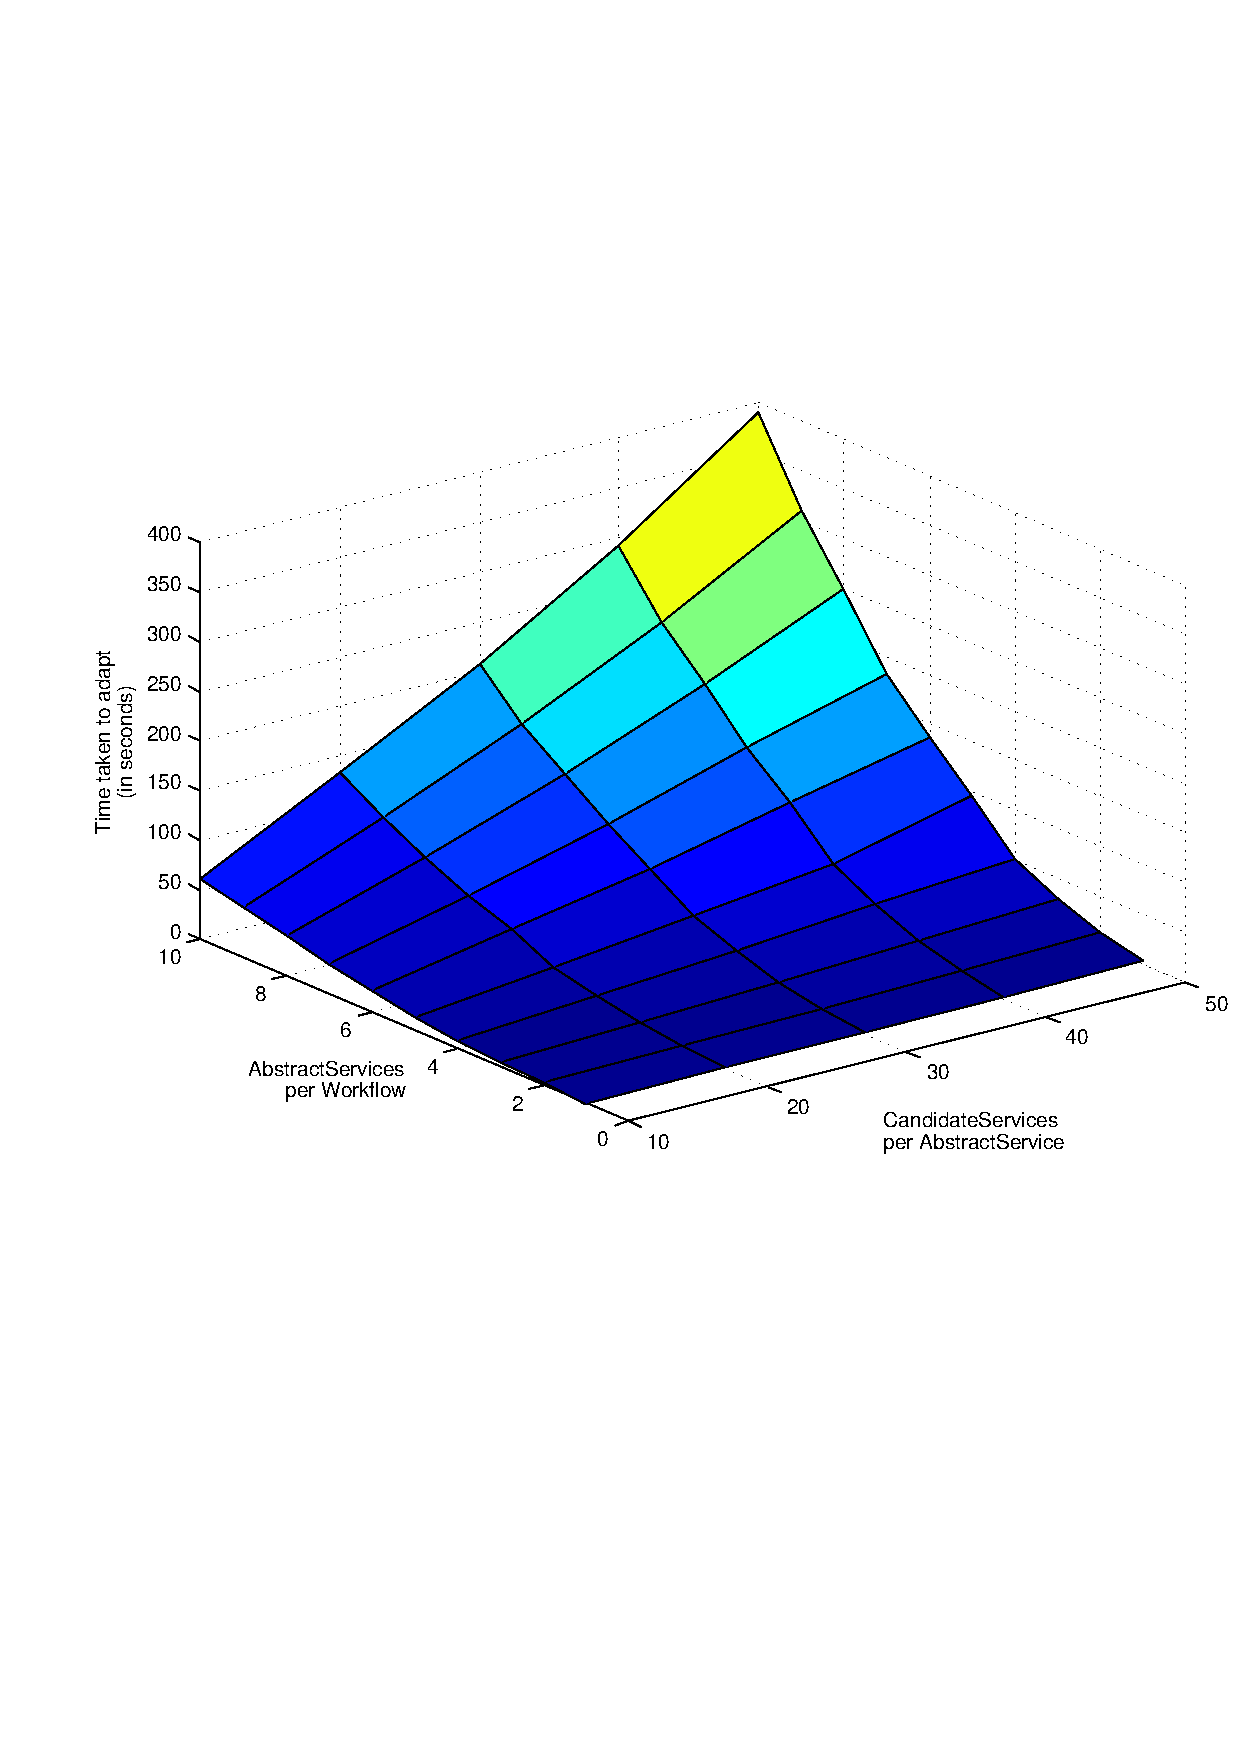
\includegraphics[clip, trim=3cm 11cm 2cm 7cm,scale=0.45]{graphs/scaling_time_task_candidates.pdf}
	\caption{Both AbstractServices and CandidateServices increase \label{fig:task_and_candidate_scaling}}
\end{figure}

We see that clobmas is more sensitive to the number of AbstractServices in the workflow, than to the number of CandidateServices available per AbstractService (see figures \ref{fig:task_per_svc}, \ref{fig:svc_per_task} and \ref{fig:task_and_candidate_scaling}). The time taken to adapt increases faster when the number of AbstractServices in the workflow increases, as compared to the number of CandidateServices per AbstractService. From the perspective of individual applications inside clobmas, this is a good thing since the workflow of an individual application does not change, as often as the number of CandidateServices available. Since the time to adapt does not rise dramatically, with the rise in availability of CandidateServices, applications have a greater chance of adapting quickly and attaining their required QoS.

\textbf{CandidateServices Vs. QoS attributes per Service:}
As the number of applications that use clobmas increase, it will have to make a decision on whether to increase the number of CandidateServices per AbstractService, or increase the number of QoS attributes available per AbstractService. Regardless of the business implications of each, both will have an impact on the scalability of clobmas. In the following figures (see fig \ref{fig:svc_per_qos} and \ref{fig:qos_per_svc}), we see that each variable affects the time-to-adapt in approximately the same way. There is a slight difference in the slope of the lines, when QoS attributes are increased (as shall be seen in figure \ref{fig:svc_and_qos_scaling}).

\begin{figure}[htbp]
	\begin{minipage}[b]{0.4\linewidth}
		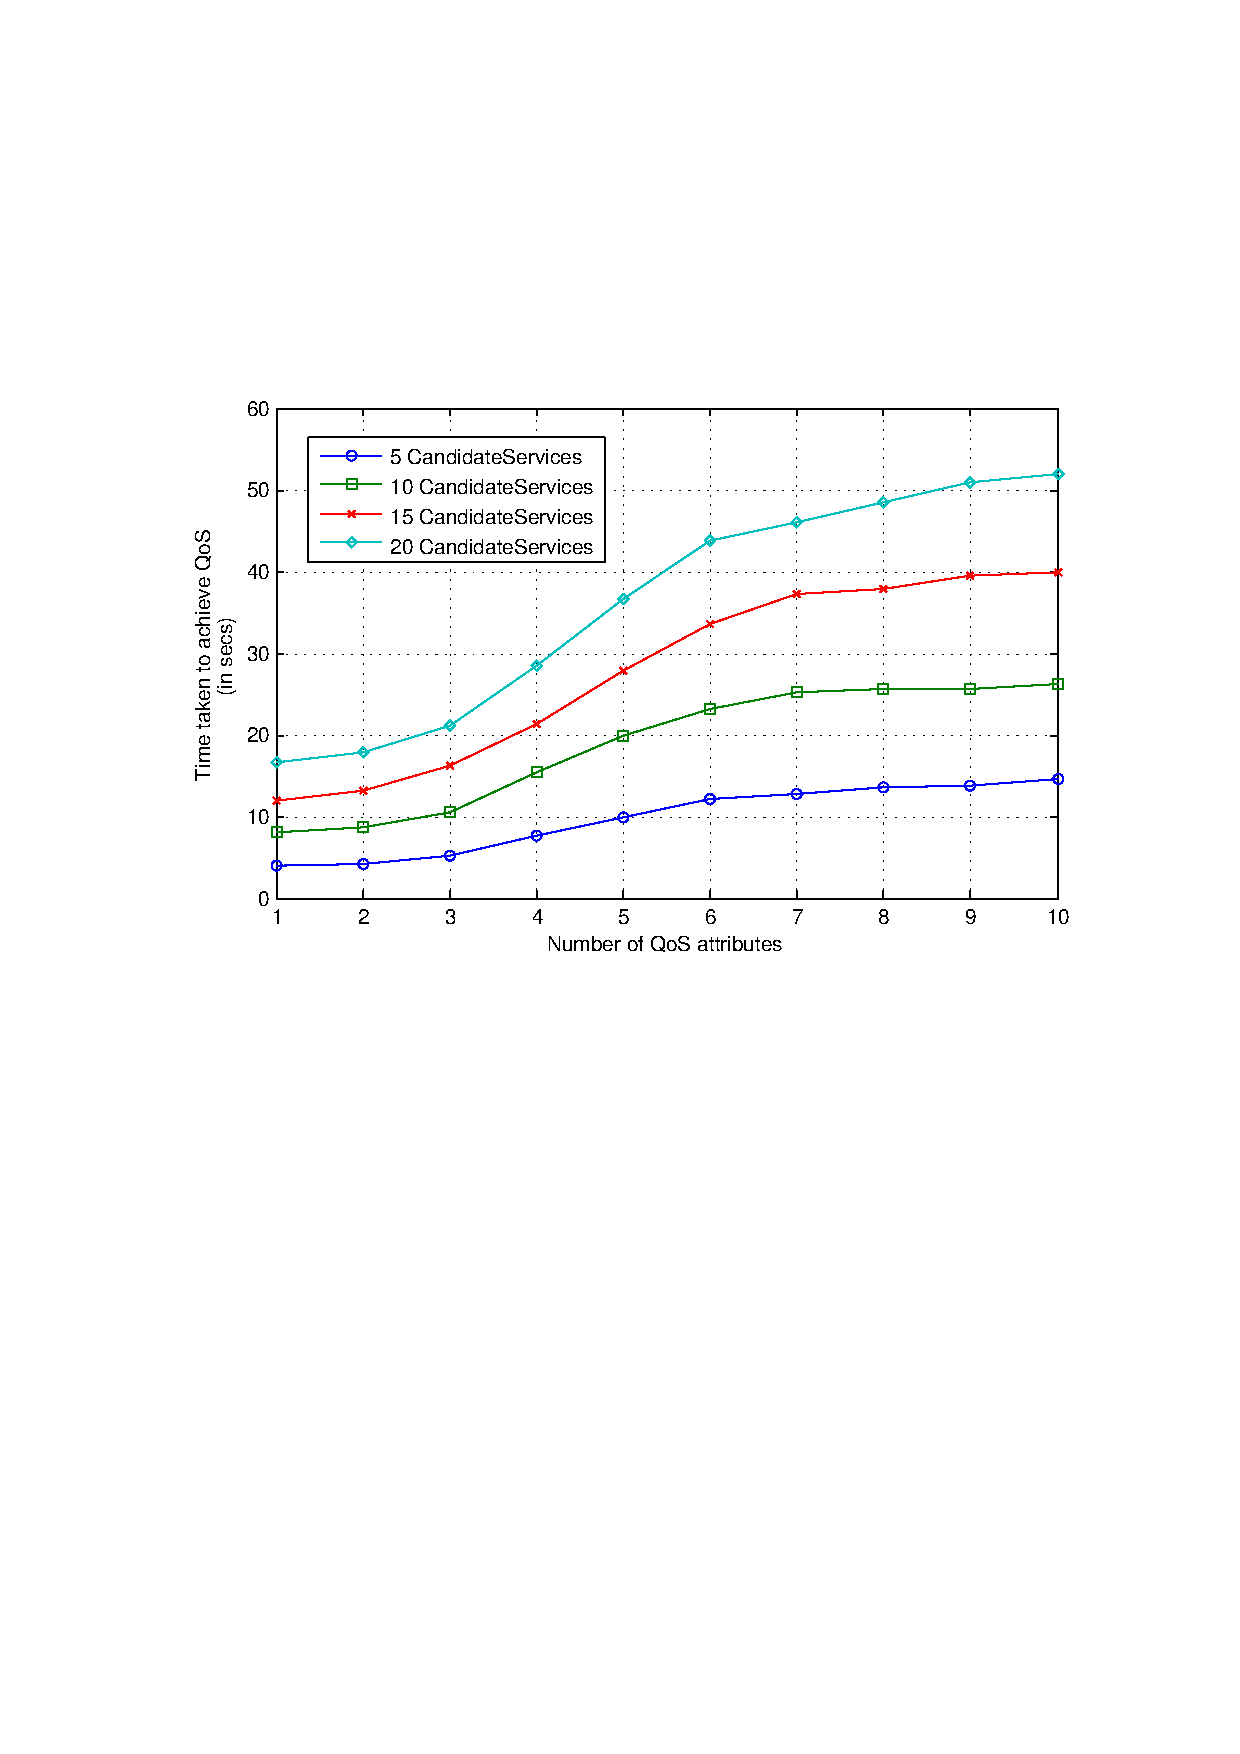
\includegraphics[clip, trim=4cm 14cm 2cm 6cm, scale=0.3]{graphs/5_10_15_20_svc_per_qos_scaling.pdf}
		\caption{CandidateServices increase \label{fig:svc_per_qos}}
	\end{minipage}
	\hspace{0.9cm}
	\begin{minipage}[b]{0.4\linewidth}
			\vspace{0.3cm}
		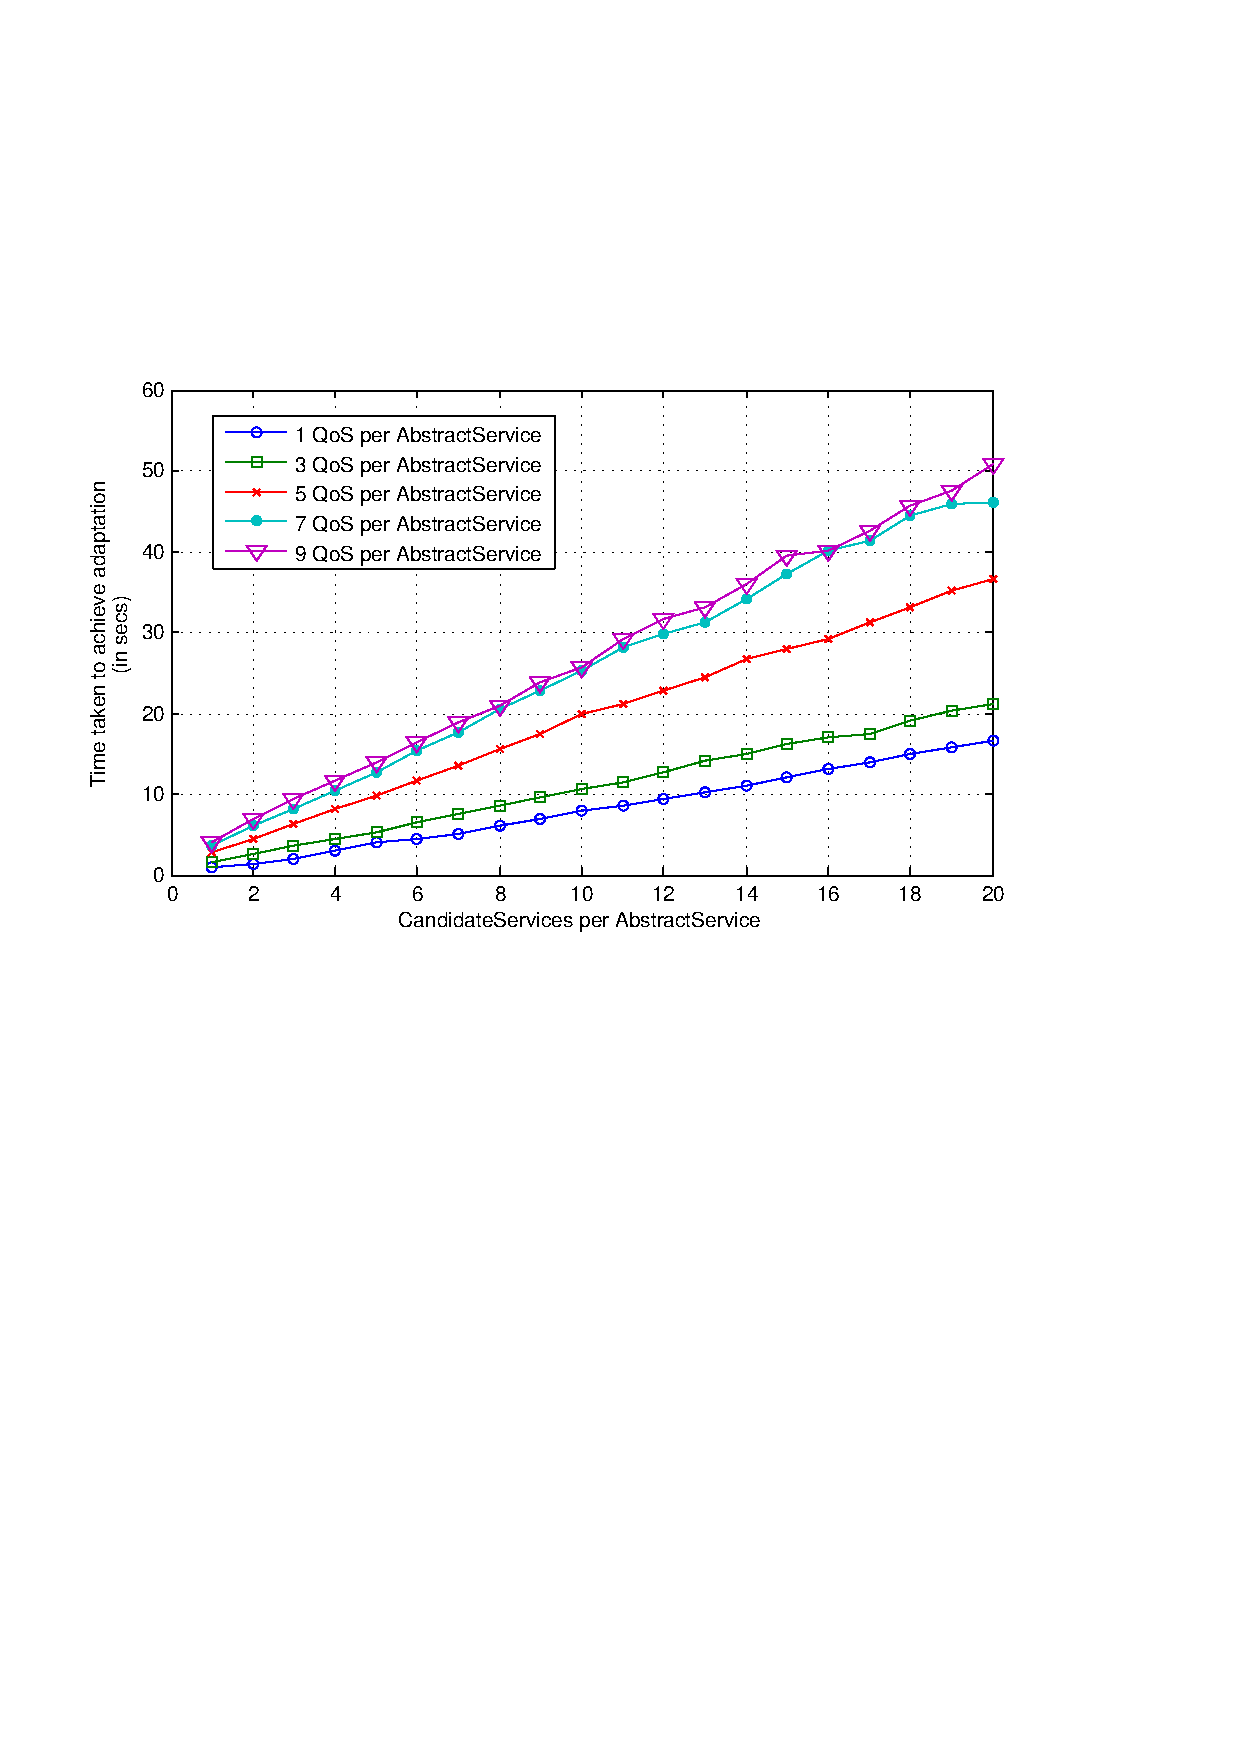
\includegraphics[clip, trim=2cm 14cm 2cm 6cm, scale=0.3]{graphs/1_3_5_7_9_qos_per_svc_scaling.pdf}
		\caption{QoS increase \label{fig:qos_per_svc}}
	\end{minipage}
\end{figure}

\begin{figure}[htbp]
\centering
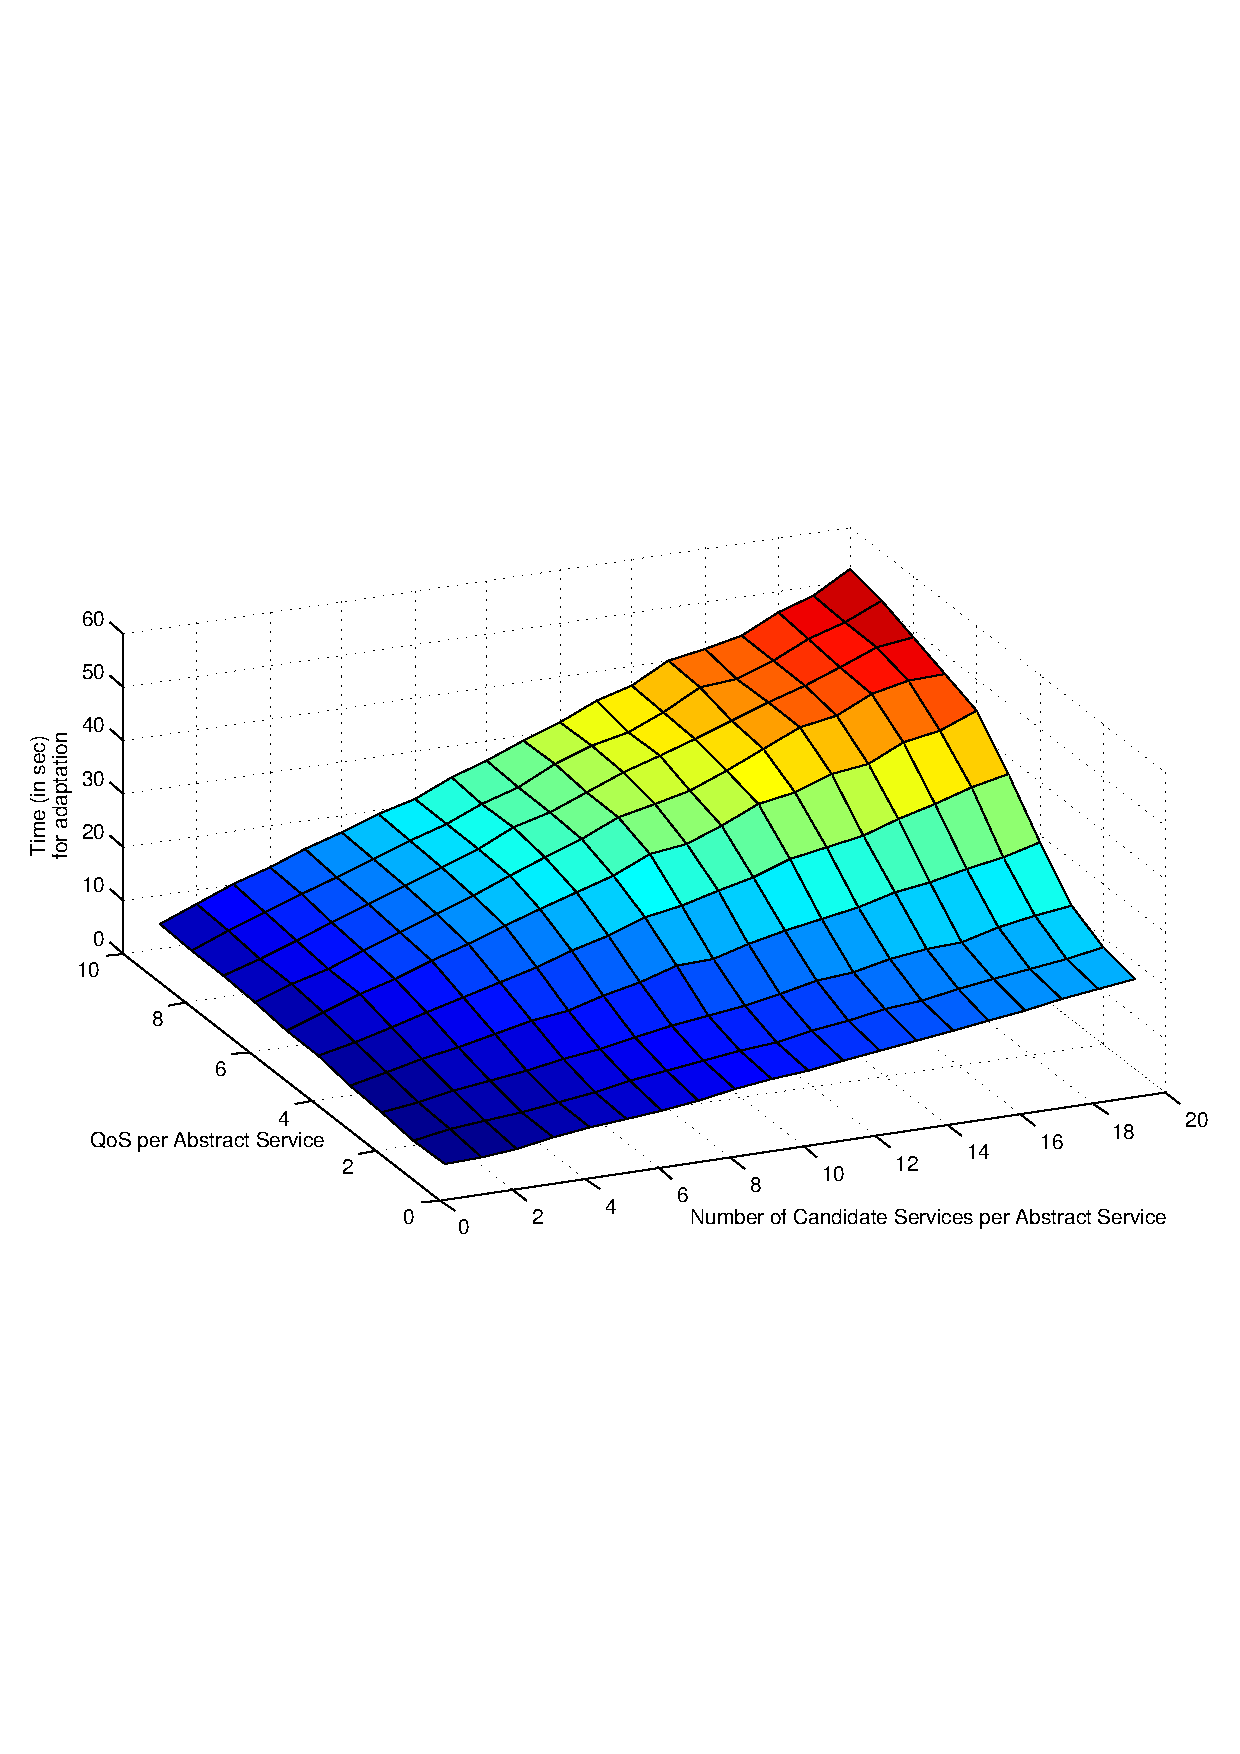
\includegraphics[clip, trim=2cm 9cm 2cm 12cm, scale=0.5]{graphs/scaling_time_svcs_qos.pdf}
\caption{Both CandidateServices and QoS increase \label{fig:svc_and_qos_scaling}}
\end{figure}

We see from figure \ref{fig:svc_and_qos_scaling} that the slope of QoS axis is greater than that of CandidateServices. That is, time taken for adaptation increases faster when QoS attributes increase, as compared to the number of CandidateServices available per AbstractService.


\subsubsection{The Cost of Decentralization}
As discussed in \cite{Eymann2003Decentralized}, an auction-based mechanism, by default, leads to a centralized mechanism. The auctioneer becomes a single point of failure, and thus leads to decreased robustness. This can be remedied by introducing multiple auctioneers. In clobmas, we use multiple markets for each AbstractService. This ensures that even if one market is non-functional, the others continue to function. Decentralization of markets comes at a cost. Buyer Agents have to choose which market to place their bids, to place them in multiple markets or a single market. Placing bids in multiple markets increases the chances of getting Candidate Services, but it also places a greater computational load on the Buyer Agent in terms of decision making. We currently choose markets randomly.\\
\textbf{CandidateServices Vs. Number of Markets:} Does decentralization affect time taken for adaptation or number of CandidateServices? In other words, should clobmas increase the number of CandidateServices available per market? Or would it be better to increase the number of markets? Increasing the number of markets increases the robustness of the system. 

\begin{figure}[htbp]
		\begin{minipage}{0.4\linewidth}
			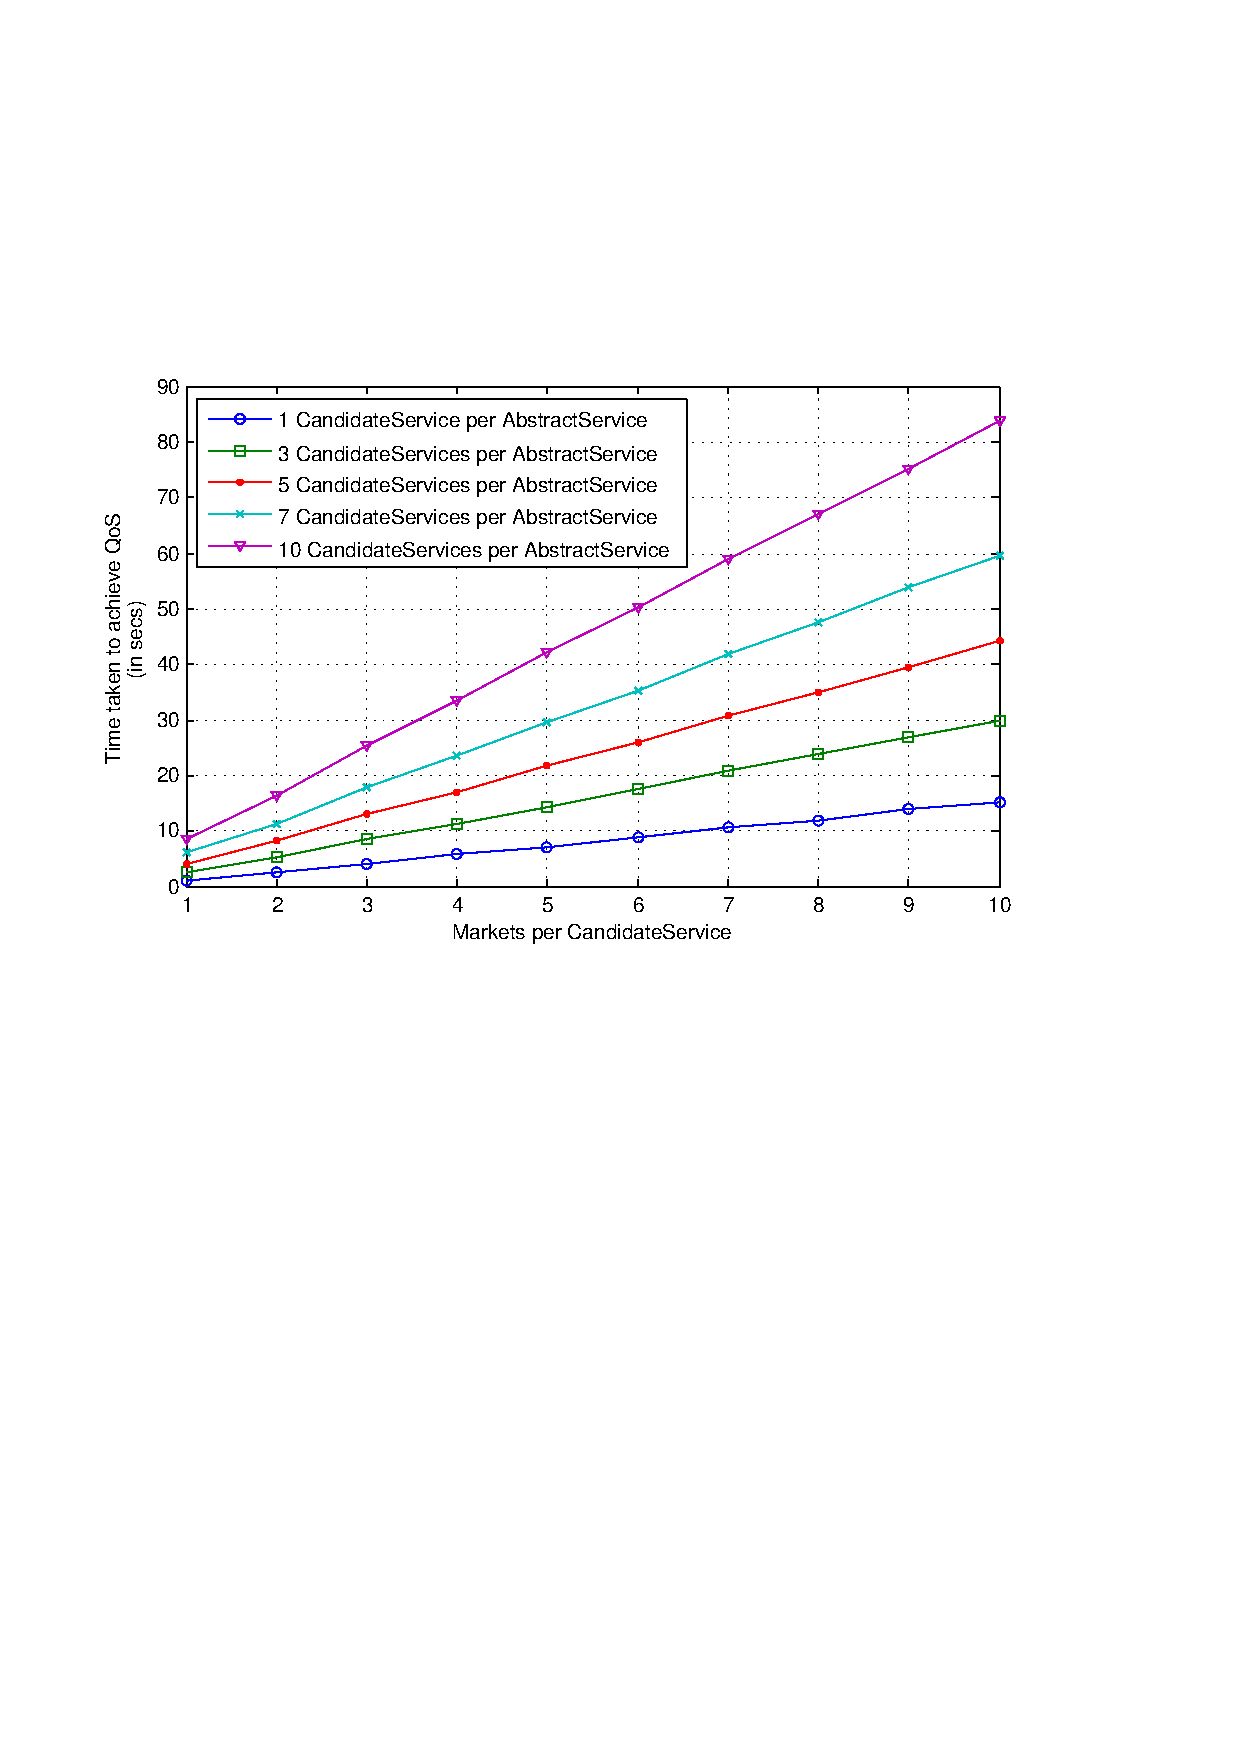
\includegraphics[clip, trim=4cm 14cm 6cm 6cm, scale=0.3]{graphs/1_3_5_7_10_svc_per_mkt_scaling.pdf}
			\caption{CandidateServices increase per Market\label{fig:svc_per_mkt}}		
		\end{minipage}
		\hspace{0.9cm}
		\begin{minipage}{0.4\linewidth}
			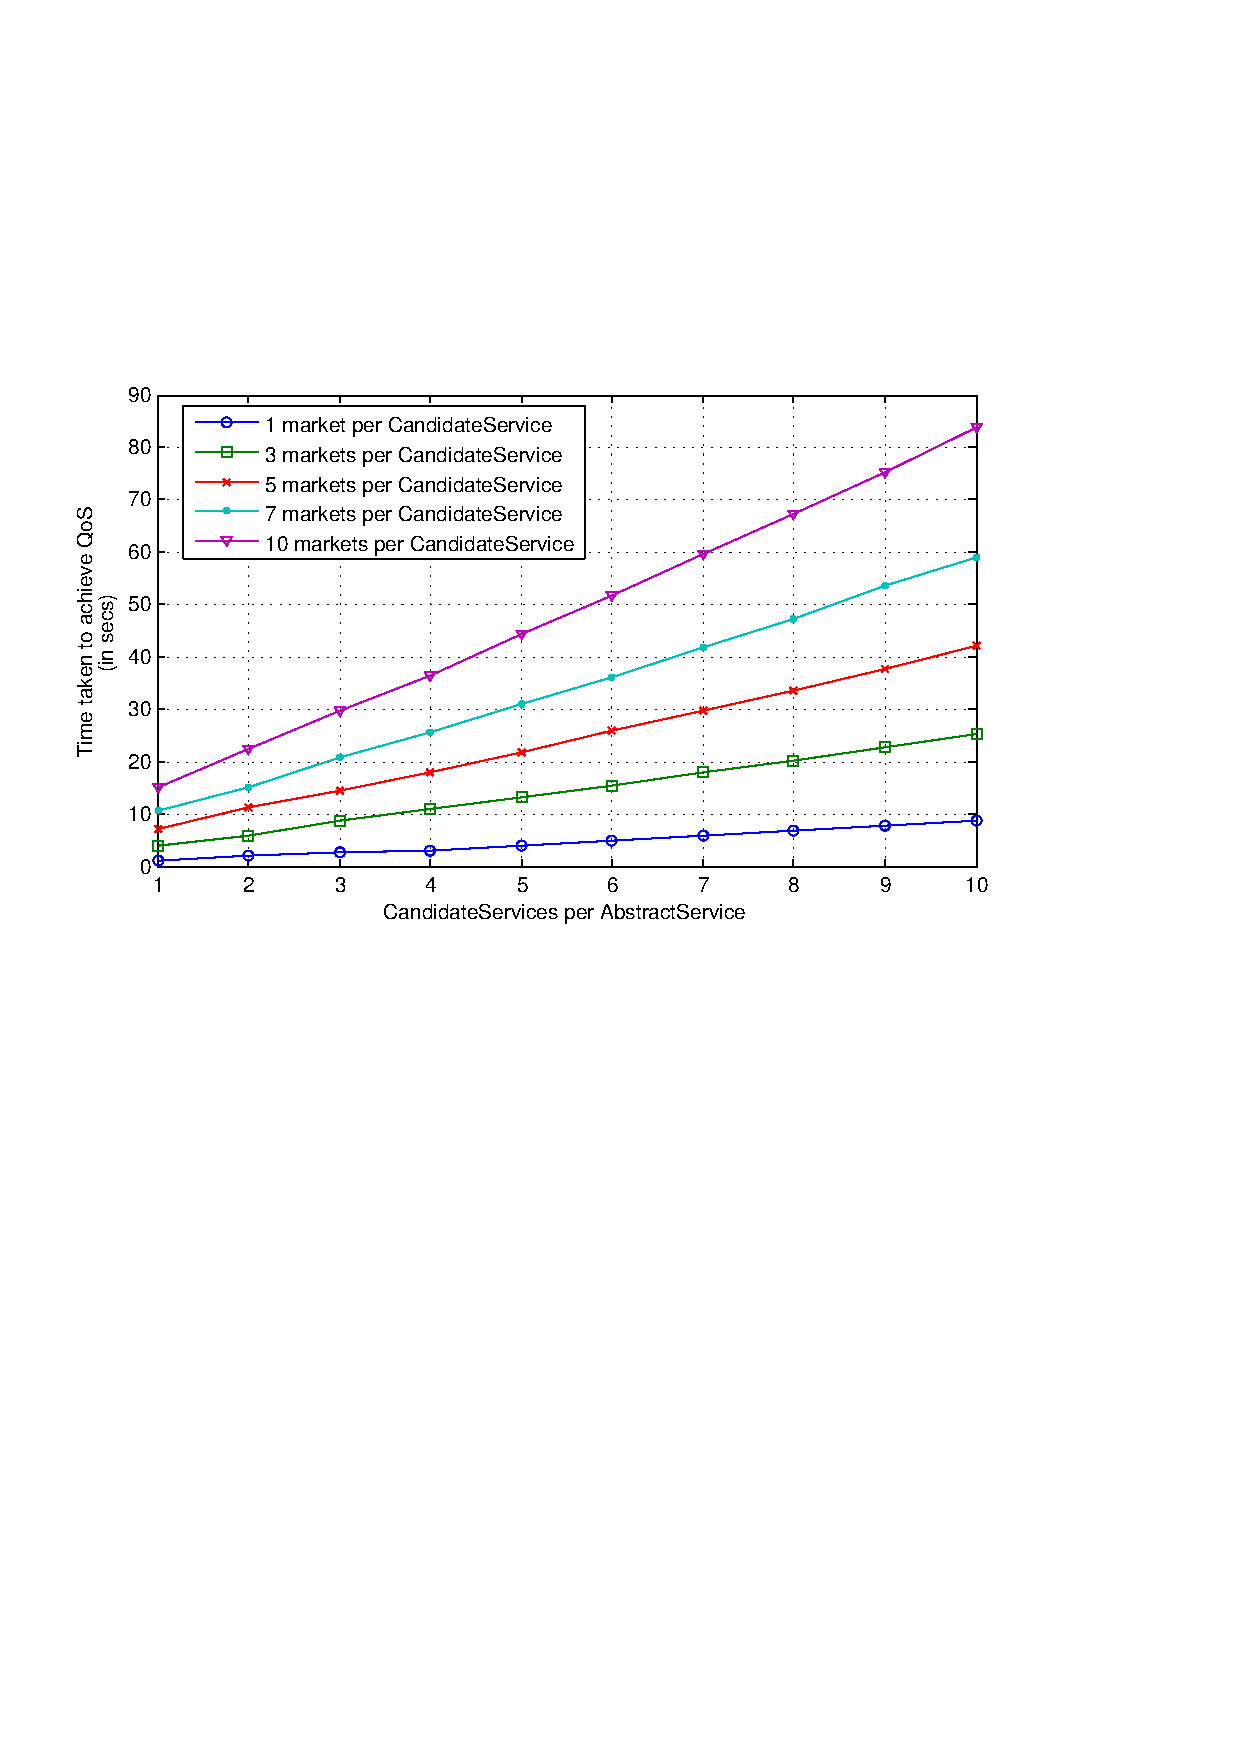
\includegraphics[clip, trim=2cm 14cm 6cm 6cm, scale=0.3]{graphs/1_3_5_7_10_mkts_per_svc_scaling.pdf}
			\caption{Markets increase per CandidateService \label{fig:mkt_per_svc}}
		\end{minipage}		
\end{figure}

We see from figures \ref{fig:svc_per_mkt} and \ref{fig:mkt_per_svc} that the slopes of the lines is almost linear. That is, increasing the number of CandidateServices \textit{vis-a-vis} increasing the number of markets does not make a significant difference to the time-to-adapt.

\begin{figure}[htbp]%
	\centering
	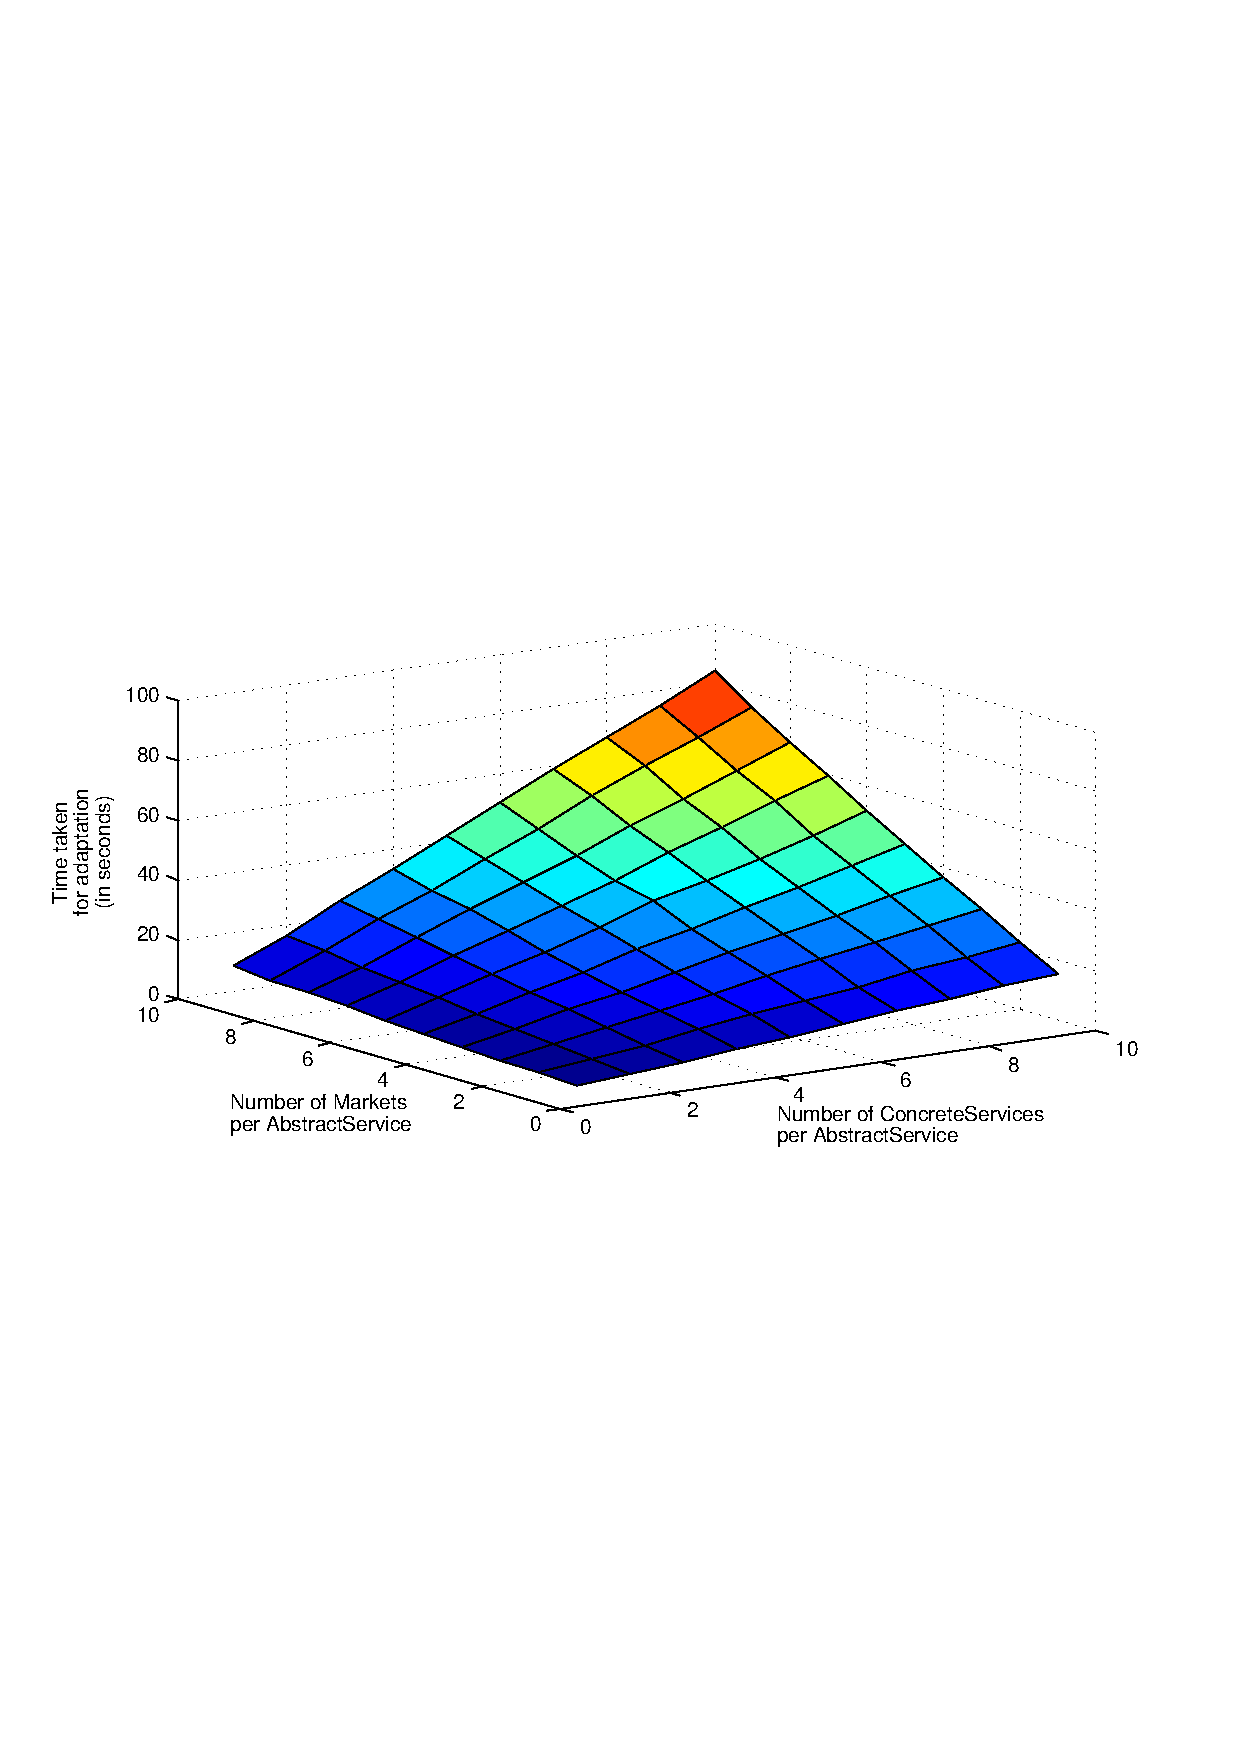
\includegraphics[clip, trim=2cm 10cm 2cm 10cm, scale=0.5]{graphs/scaling_time_svcs_mkts.pdf}
	\caption{Both Candidate Services and Markets increase \label{fig:svc_and_mkts_scaling}}%
\end{figure}

Hence, the decision to increase robustness does not negatively impact the time-to-adapt exhibited by clobmas. \\
\textbf{QoS attributes Vs. Number of Markets:}
Next we look at how QoS attributes affect the time-to-adapt \textit{vis-a-vis} the number of markets. 

\begin{figure}[htbp]
		\begin{minipage}{0.4\linewidth}
			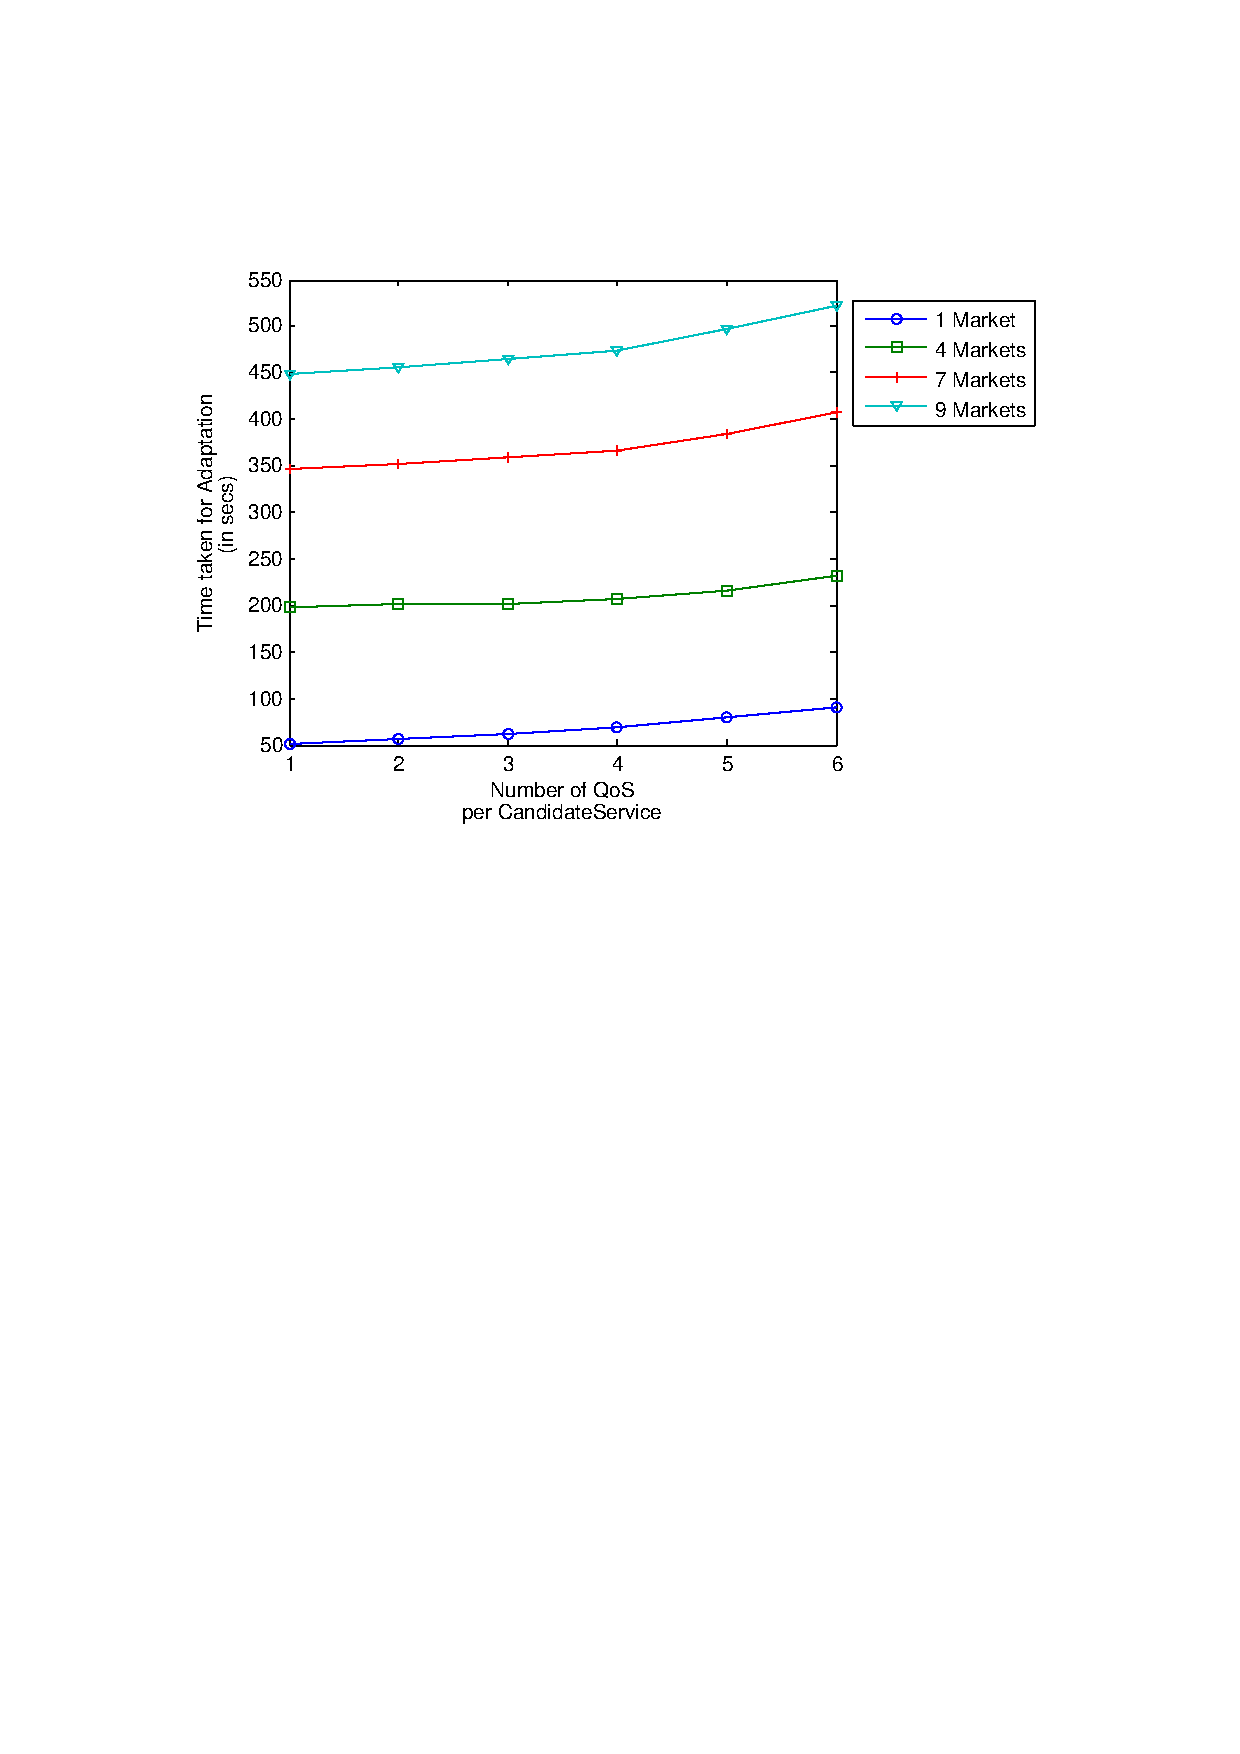
\includegraphics[clip, trim=4cm 16cm 6cm 4cm, scale=0.4]{graphs/1_4_7_9_mkts_per_qos.pdf}
			\caption{Markets increase per QoS\label{fig:mkt_per_qos}}		
		\end{minipage}
		\hspace{0.9cm}
		\begin{minipage}{0.4\linewidth}
			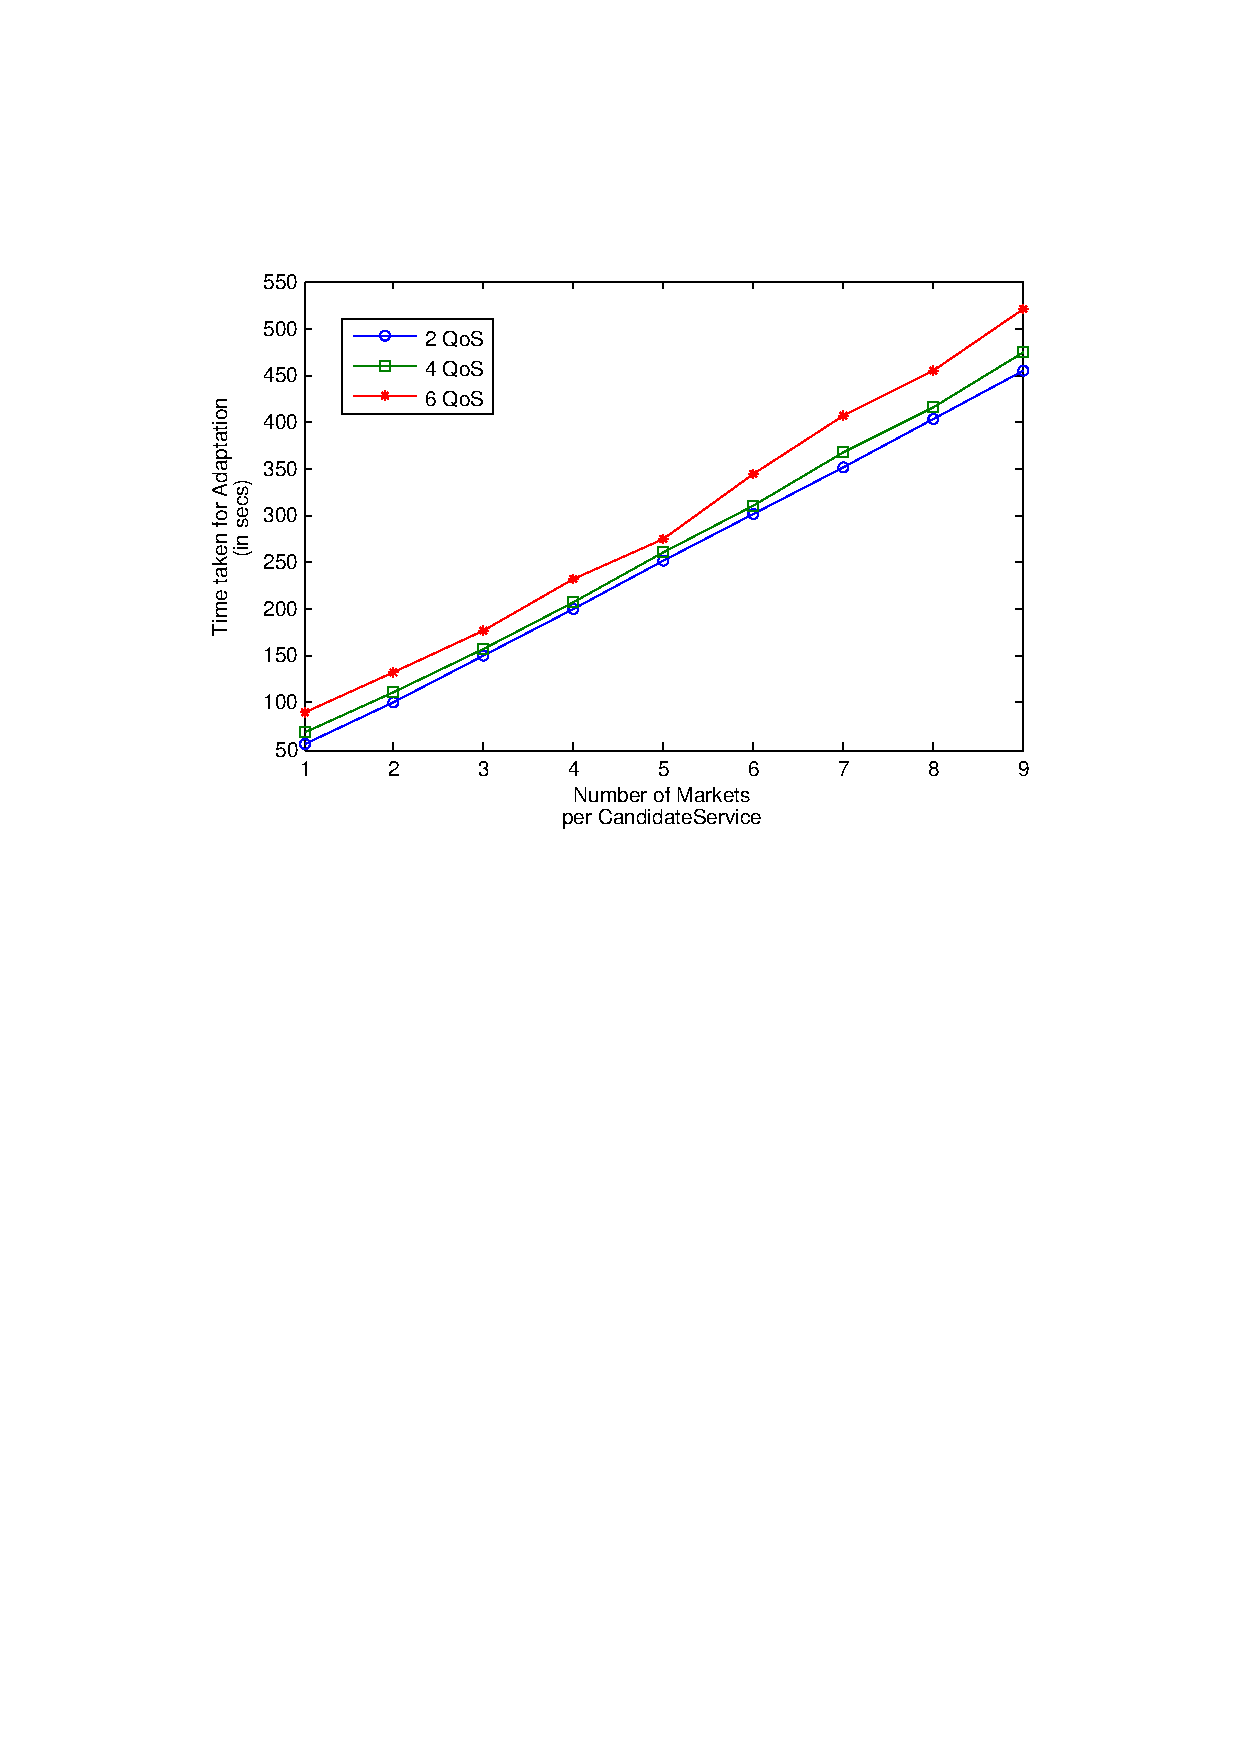
\includegraphics[clip, trim=2cm 16cm 6cm 4cm, scale=0.4]{graphs/2_4_6_qos_per_mkt_scaling.pdf}
			\caption{QoS increase per Market \label{fig:qos_per_mkt}}
		\end{minipage}		
\end{figure}

We see that increasing the number of markets adds a constant amount of time to the adaptation process. On the other hand, increasing the number of QoS per CandidateService causes a non-proportional increase in the time taken. In other words, increasing the number of QoS per CandidateService is more expensive than increasing the number of markets. 

\begin{figure}[htbp]
	\centering
	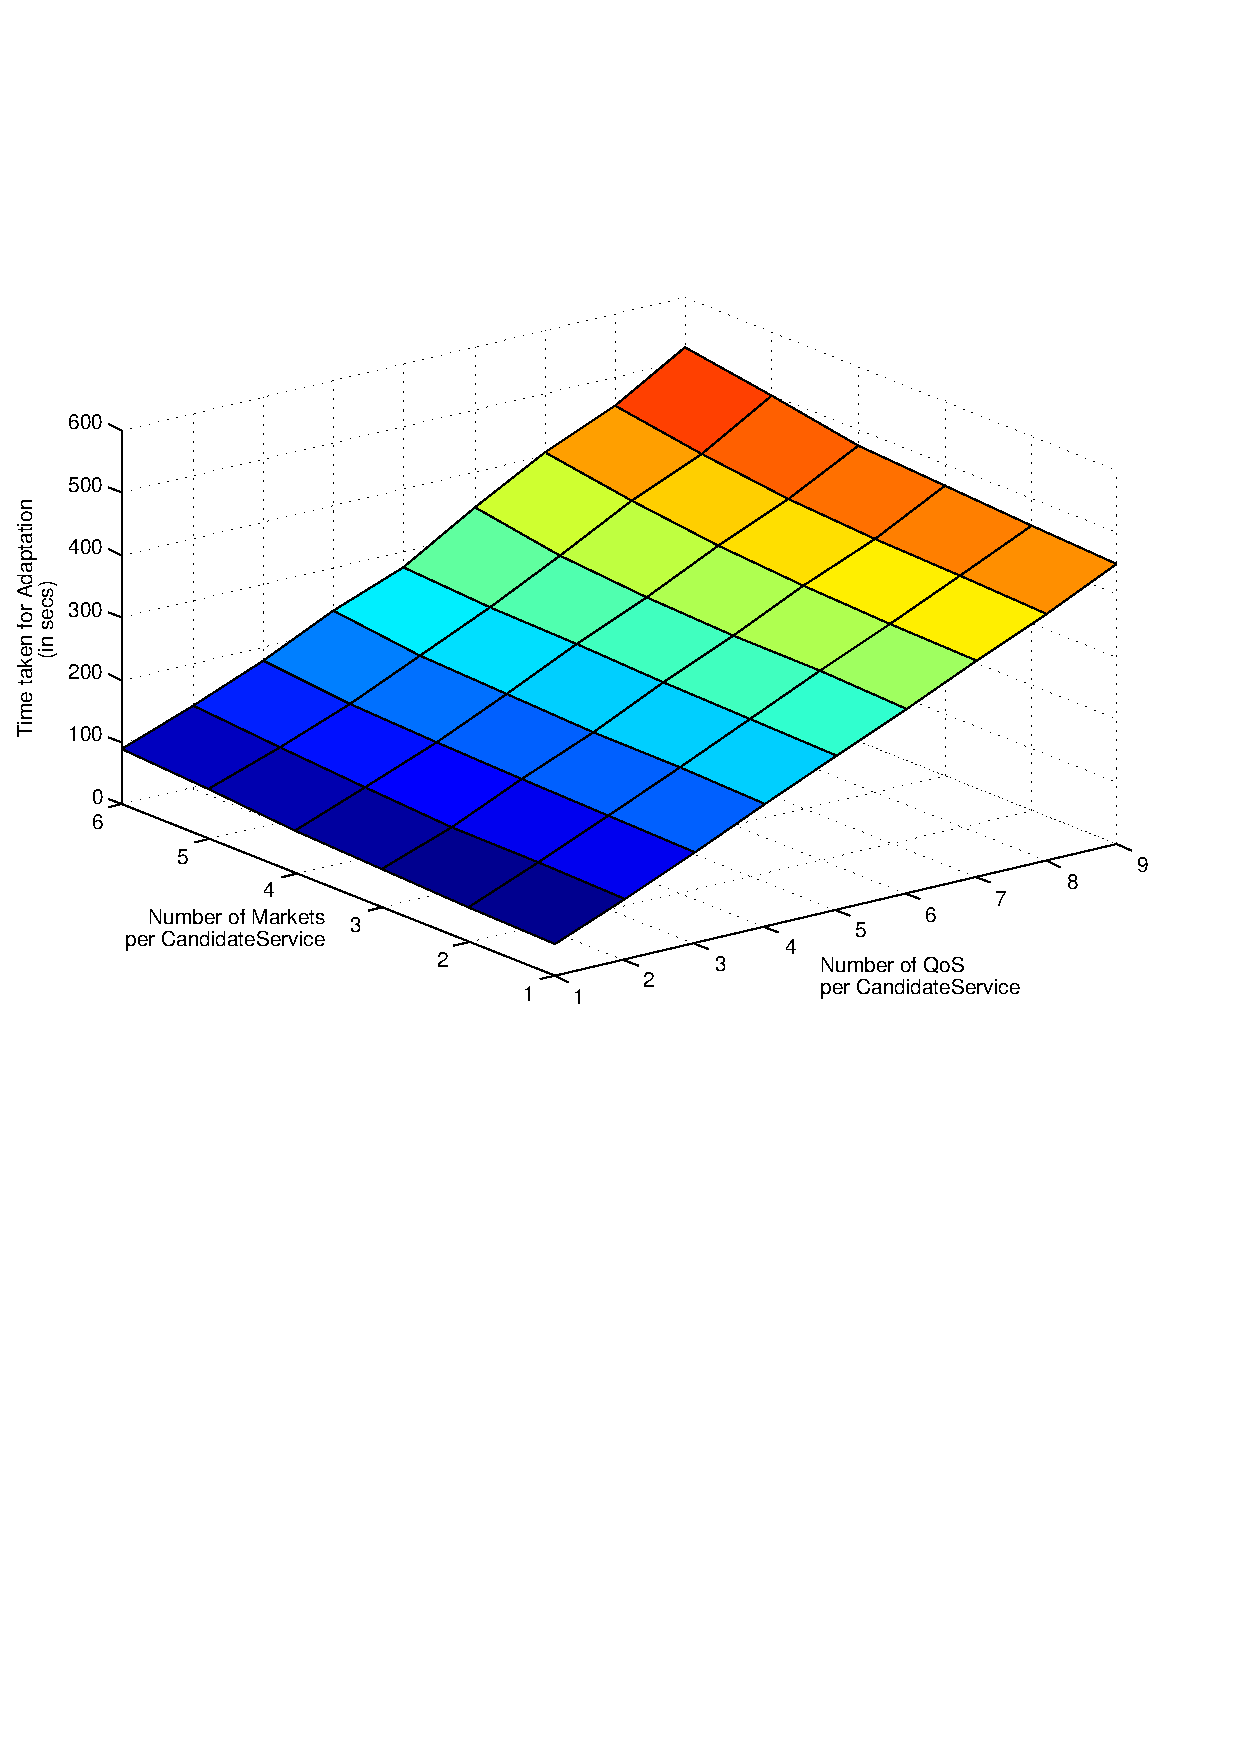
\includegraphics[clip, trim=2cm 12cm 2cm 6cm, scale=0.45]{graphs/scaling_time_qos_mkts.pdf}
	\caption{Both QoS attributes and markets increase \label{fig:qos_and_mkts_scaling}}
\end{figure}

\subsection{QoS Monitoring Engine}
Monitoring the actual QoS exhibited during runtime by the CandidateService, is beyond the scope of the system. We assume that all the agents agree on the monitoring of a CandidateService, by a specific monitoring mechanism. This could be market-specific or domain specific. The monitoring of QoS cannot be done by our mechanism, since it needs to be neutral. The monitoring mechanism will be used by both parties: BuyerAgent and SellerAgent. The BuyerAgent needs to know whether the SellerAgent's service is providing the QoS that it promised. The SellerAgent needs to know that the BuyerAgent's application is not abusing the service. Zeng \cite{Zeng2007Monitoring}, and Michlmayer\cite{Michlmayr2009Comprehensive} are good examples of online QoS monitoring. Zeng et al. classify QoS metrics into three categories: (a) Provider-advertised (b) Consumer-rated, and (c) Observable metrics. They provide an event-driven, rule-based model where designers can define QoS metrics and their computation logic (in terms of Event-Condition-Action rules), for observable metrics. These are then compiled into executable statecharts, which provide execution efficiency in computing QoS metrics based on service-events that are observed. \\
Michlmayer et al. provide their QoS monitoring as a \textit{service runtime environment}. This service runtime environment addresses service metadata, QoS-aware service selection, mediation of services and complex event processing. The authors propose two mechanisms to monitor QoS: (a) a client-side approach using statistical sampling, and (b) a server-side approach using probes that are present on the same host as the service. The client-side approach is non-intrusive, in terms of not needing access to the service's host. \\
Both approaches, Zeng and Michlmayer, use an event-based mechanism to detect QoS values, and SLA violations, if any. This fits in neatly with our need for a non-intrusive, third-party based QoS Monitoring Engine. Our mechanism is agnostic to the actual QoS monitoring mechanism, that is used. 



%In none of the papers that we surveyed (in section \ref{dynamic_wsc}), did we find a single rigorous definition of what it would mean for a dynamic service composition technique to be scalable . In the absence of such a definition, it is difficult to judge, whether a technique is really scalable or not. To alleviate the problem of capricious definitions of scalability, we use a definition of scalability from \cite{Duboc2007framework}: \textit{a quality of software systems characterized by the causal impact that scaling aspects of the system environment and design have on certain measured system qualities as these aspects are varied over expected operational ranges}.\\
%According to \cite{Duboc2007framework}'s definition, when these variables change, they have an impact on the system's qualities. In our case, the system qualities that we want to measure are:
%	\begin{enumerate}
%		\item Efficacy, measured as a fraction of the total applications that are able to achieve their required QoS
%		\item Performance, measured as the amount of time taken to select services, when critical variables vary over an expected range.
%	\end{enumerate}	 
%After a careful perusal of available literature on dynamic web-service composition, we have determined that the following variables are critical, in their effect on the performance of the service selection technique. We explicate the critical variables of the system as:
%	\begin{enumerate}
%		\item AbstractServices per workflow, 
%		\item Number of candidate services, \textit{i.e.}, the number of concrete services available per abstract service
%		\item Number of QoS values per candidate service
%	%	\item Number of end-to-end QoS constraints
%%		\item Number of markets available for acquiring concrete services
%	\end{enumerate}
	


%\textbf{Periodicity of Change}:\\
% In figures \ref{QoS_Change1} and \ref{QoS_Change2}, we compare the differences in the aggregate behaviour of all applications, when the periodicity of change of QoS is varied. In the first instance, we model all applications having independent probabilities of changing their target QoS attributes, over time. This means, any application could change its target QoS, at any point in time. In the second instance, we simulate an external event causing the applications to change their target QoS, every 25 rounds of trading.
%       \begin{figure}
%	 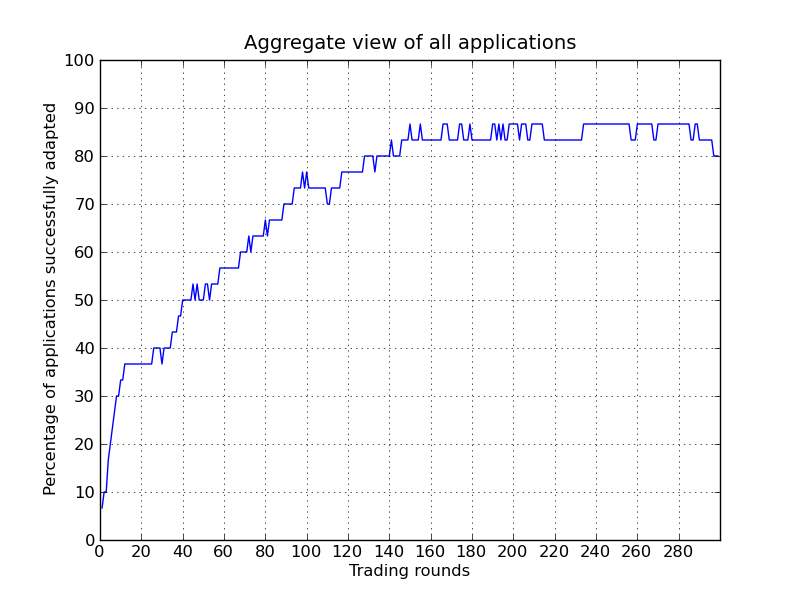
\includegraphics[width=3.8in]{graphs/probabilistic-change-to-qa.png}
%	 \caption{Each application that succeeds in reaching its target, changes its target QoS with a small probability. We see that in the aggregate, there's not much change in the percentage of applications being able to self-adapt.}
%	 \label{QoS_Change1}
%       \end{figure}
%	 \begin{figure}
%	 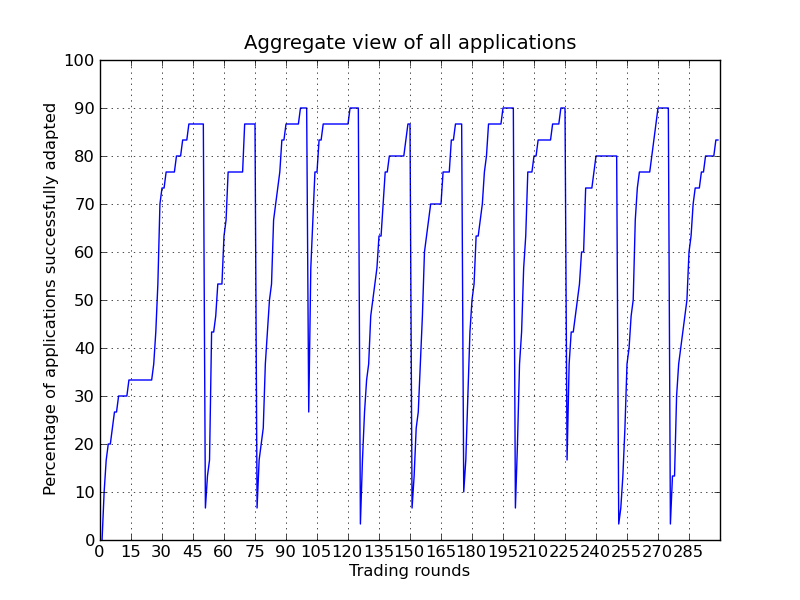
\includegraphics[width=3.8in]{graphs/periodic-change-to-qa.png}
%	  \caption{Instead of a successful application changing its QoS, every application changes its target QoS at the completion of 25 trading rounds. This makes the aggregate adaption easier to see, since the market as a whole experiences a change in demand, periodically} 
%	 \label{QoS_Change2}
%	 \end{figure} %\\ \hline
%%      \end{tabular}
%     	
%%  \end{table}
%As expected, the periodic external event causes the aggregate number of satisfied applications to drop precipitously. Interestingly, it also causes the mechanism to satisfy a much higher percentage of the total applications. This is an interesting event and needs more investigation.
%
%\subsection{Scalability Results}
%\paragraph{With regard to size of workflow}
%\paragraph{Number of candidate services}
%\paragraph{Number of QoS constraints}
%\paragraph{Number of markets}

\subsection{Discussion}
%DISCUSS PROS-AND-CONS OF ADOPTED ARCHITECTURAL STYLE. 
\subsubsection{Strengths}
A big strength of our mechanism is the high scalability that it offers. As service-oriented applications mature and cloud offerings become more standardized, it is easy to envision applications being composed out of several third-party services. In such a scenario, a mechanism that scales up to accommodate many concrete services is essential. We see that our mechanism is easily able to scale up.\\
Since the decision-making over which concrete service to instantiate is done in a de-centralized manner, the individual agents can be simple and easy to implement. \\    
Our mechanism implements a continuous adaptation scheme, thus leaving the system administrator free to attend to more critical tasks.

\subsubsection{Threats to Validity}

The set of services used to model the supply (as seen in table \ref{tbl:choice-of-services}) is deliberately seeded with services that probably will not be able to transact (e.g. $S1_{3}, S1_{54}, S3_{3}, S4_{3}$, etc.). This is done with a view to evaluating the mechanism's performance in an extreme situation. Services that advertise an availability of 79\% ($S1_{3}$) would never be acceptable.  In real life, these services would be competed out of the market, with most services differing in their QoS offerings by a marginal amount (or the price would be appropriately low, for low QoS). With a more typical scenario, our mechanism's performance would be much better, since the number of applications that are able to successfully achieve their QoS would be higher than figure \ref{fig:cda_zip_market_satisfaction}. Since the self-adaptive mechanism merely attempts to satisfy the application's QoS targets, it does not try to achieve  optimal set of concrete services, even if available. This is a trade-off that occurs between simplicity and robustness on one hand, and optimality on the other.\\

The market mechanism does not achieve the optimum, neither from the individual perspective nor from the aggregate perspective. Given the bounded rationality of our agents, we aim only to achieve a satisficing result, that is, find a solution that satisfies the constraints. 
% All satisficing problems can be trivially reformulated into optimization problems, but satisficing solutions need not be optimal solutions and vice-versa.\\

\textbf{Lack of Trust}: In any market-oriented mechanism, there is the issue of trust between the buyer of a service and the seller of a service. How does the seller reliably ensure that the buyer does not make more calls to the web-service, than the number agreed upon? How is the provenance of calls established? How does the buyer ensure that the seller provides the QoS, that it has promised in the SLA? What legal/technical recourse does it have, in case of violation of contract? These are all issues that are still open research problems. \cite{Ramchurn2005Trust} provides a good overview of these problems in the specific case of multi-agent systems. However, a good amount of research needs to be done, before all issues are acceptably resolved to the satisfaction of both, buyer and seller.\\
%\textbf{QoS Monitoring by External Entities}: Monitoring of QoS by third-party engines solve some of the trust issues discussed above, but introduce new ones. 
%
%\textbf{QoS Monitoring}: Monitoring a web-service for an SLA violation is a topic of research in its own right. There have been several attempts in this direction, most notably from \cite{Chau2008Automatinga, Michlmayr2009Comprehensive, Raimondi2008Efficient} and \cite{Skene2004Precise} In this paper, we do not attempt to devise our own scheme for QoS monitoring. Rather, we assume that one of the methods outlined in the afore-mentioned research, is used. Zeng \cite{Zeng2007Monitoring}, and Michlmayer\cite{Michlmayr2009Comprehensive} are good examples of online, event-based QoS monitoring.\\
%Zeng et al. classify QoS metrics into three categories: (a) Provider-advertised (b) Consumer-rated, and (c) Observable metrics. They provide an event-driven, rule-based model where designers can define QoS metrics and their computation logic (in terms of Event-Condition-Action rules), for observable metrics. These are then compiled into executable statecharts, which provide execution efficiency in computing QoS metrics based on service-events that are observed. \\
%Michlmayer et al. provide their QoS monitoring as a \textit{service runtime environment}. This service runtime environment addresses service metadata, QoS-aware service selection, mediation of services and complex event processing. The authors propose two mechanisms to monitor QoS: (a) a client-side approach using statistical sampling, and (b) a server-side approach using probes that are present on the same host as the service. The client-side approach is non-intrusive, in terms of not needing access to the service's host. \\
%Both approaches, Zeng and Michlmayer, use an event-based mechanism to detect QoS values, and SLA violations, if any. This fits in neatly with our need for a non-intrusive, third-party based QoS Monitoring Engine. Our mechanism is agnostic to the actual QoS monitoring mechanism, that is used.\\

\textbf{Simulation Effects}: Any simulation model is a constrained version of reality, and as such, results from simulations should always be taken with a pinch of salt. Given this caveat, simulations help us carry out controlled experiments that would be too cumbersome or expensive to carry out in reality. Simulation toolkits are a valuable mechanism for testing out new, and sufficiently different ideas. CloudSim \cite{Buyya2009Cloudbus} is a toolkit that aims to make simulations of clouds easier to perform, and in the ideal case, we would have liked to implement our ideas on it. However, at its current level, it is insufficient to capture market mechanisms and multiple types of QoS attributes. In future, we aim to port our market-model to CloudSim, so as to enable richer modelling.

\section{Related Work}
    
\subsection{Dynamic Composition of Web-services} \label{dynamic_wsc}
There has been a plethora of work on dynamic composition of web-services. Much early work has been done in AgFlow \cite{Zeng2001AgFlow} on Quality-Aware composition of web-services \cite{Benatallah2002Declarative} and \cite{Zeng2003Quality}. The authors propose a per-service-class optimisation as well as a global optimisation using integer programming.\\
\cite{Canfora2005approach} proposed a genetic algorithm based approach where the genome length is determined by the number of abstract services that require a choice to be made. Constraints on QoS form a part of the fitness function, as do cost and other QoS attributes. A big advantage of GA-based approach is that it is able to handle non-linear constraints, as opposed to integer programming. Also, it is scalable when the number of concrete services per abstract service increase.\\
\cite{Alrifai2010Selecting} propose an interesting mechanism for cutting through the search space of candidate web-services, by using skyline queries. Skyline queries identify \textit{non-dominated} web-services on at least one QoS criteria. A \textit{non-dominated} web-service means, a web-service that has at least one QoS dimension in which it is strictly better than any other web-service and at least equal on all other QoS dimensions. Determining skyline services for a particular abstract service, requires pairwise comparisons amongst the QoS vectors of all the concrete services. This process can be expensive if the number of candidate concrete services is large. Alrifai et al. consider the case where the process of selecting skyline services is done offline. This would lead to an inability to adjust to changing conditions of available services and their associated QoS values. 	
\cite{Zhang2010QoS-Based} propose an interesting method to achieve a good set of concrete services, using Ant Colony Optimization (ACO). ACO involves creating virtual ants that mimic the foraging behaviour of real ants. The search space of optimal concrete services is modelled as a graph, with sets of concrete services as vertices and edges being all the possible connections between different concrete service sets. The ants attempt to complete a traversal of the graph, dropping pheromones on the edge of each concrete service visited. The path through the graph that accumulates the most pheromones represents the near-optimal path of services to use.
Our approach differs from the above approaches in two respects:
 \begin{enumerate}
     \item Consideration of time as a factor: In practice, the optimal set of concrete services may not be available at the time instant that an application is searching. The set of service providers changes with time, as does the set of service consumers. This means that the optimal matching of service providers to consumers changes with time. The approaches above do not take this into account.
     \item Optimality not considered: Due to the infeasibility of computing the optimal set (being NP-hard), we concentrate on finding a good solution, rather than an optimal one. A good solution is one that does not violate any QoS constraints and meets the cost constraint within a certain margin.
 \end{enumerate}

\subsection{Self-Adaptation}
Applications that use dynamic service composition should be able to continuously monitor their current QoS levels and make adjustments when either the demand for QoS changes or the cost constraint changes. The application should thus be able to respond to both internal as well as external stimuli, to trigger a change in its constituent web-services. This change needs to be both timely, as well as correct, \textit{i.e.}, the new set of services should not violate any of the application's QoS constraints, and the change should happen as fast as possible.\\
Self-Adaptation in software systems is the achievement of a stable, desirable configuration, in the presence of varying stimuli. These stimuli may be environmental (in the form of workload, failure of external components, etc.) or internal (failure of internal components, changed target states, etc.). Given that the range of stimuli that affect a software system is wide, Self-Adaptation has come to mean an umbrella term that covers multiple aspects of how a system reacts\cite{Salehie2009Self-adaptive}:
	\begin{enumerate}
	   \item Self-Awareness
	\item Context-Awareness
	\item Self-Configuring
	\item Self-Optimizing
	\item Self-Healing
	\item Self-Protecting 
	\end{enumerate}
However, most approaches to self-adaptation follow a common pattern: Monitor -- Analyze -- Plan -- Execute, connected by a feedback loop. There are two approaches to self-adaptation: centralized and de-centralized.  
In a centralized self-adaptive system, the analysis and planning part are concentrated in one entity. This form of self-adaptation has the advantage of cohesiveness and low communication overhead as compared to a decentralized mechanism. The analysis and the plan can be communicated to the effectors, and feedback from obeying the plan is communicated back through the monitors (or sensors). Rainbow\cite{Cheng2006Architecture-based} and \textit{The Autonomic Manager}\cite{IBM2006Architectural} are classic examples of centralized self-adaptation.\\
Decentralized self-adaptation, on the other hand, distributes the analysis, planning or the feedback mechanism amongst different parts of the adapting system. This automatically implies a communication overhead, since all constituent parts must coordinate their actions. However, it also provides for robustness in the presence of node failure and scalability of application size. \cite{Cheng2009Softwarea} have advocated that the feedback loop, which is a critical part of the adaptation, be elevated to a first-class entity in terms of modelling, design and implementation. Although, this would allow for reasoning about properties of the adaptation, there are no systems that we currently know of, that provide an explicit focus on the feedback loop. Most decentralized self-adaptation systems are typically realised as a multi-agent systems wherein the agents are autonomous in their environments and implement strategies that collectively move the entire system into a desirable state. \cite{Cheng2005Making} have advocated separating the functional part of the system from the adaptive part, thus allowing for independent evolution of both. \cite{Baresi2008Towards} describes such a system, where adaptation is considered as a cross-cutting concern, and not a fundamental part of system computation. Baresi et al. use aspect-oriented programming to implement the Monitor and Execute part of the MAPE loop. They implement distributed analysis and planning by dividing the self-adaptive system into \textit{supervised elements}, that perform the business logic of the application and \textit{supervisors} that oversee how the supervised components behave and plan for adaptation. Aspect-probes form the sensors and actuators that link the supervised elements to the supervisors. \\
\cite{Di2005Self-organization} describe another interesting approach to decentralized self-adaptation, through self-organization. DiMarzo et al. take a bio-inspired approach and use principles of holons (and holarchy) and stigmergy to get agents in a manufacturing department to perform coordination and control. A holon is defined by \cite{Koestler1990Ghost} to be both a part and a whole. Therefore, an agent is both autonomous as well as a part of a hierarchy, which influences it. The essential idea in their work is that with such structures, order emerges from disorder, as simple interactions build on each other, to produce progressively complex behaviour.\\
\cite{Weyns2010decentralized} study a decentralized self-healing system and a QoS-driven self-optimized deployment framework. Weyns et al.'s approach is the nearest to ours. They suggest multiple decentralized models which feed into decentralized algorithms, which are in turn analyzed by decentralized analyzers. These analyzers then individually direct local effectors to make changes to the host system.\\
These approaches, while interesting, have not explicitly considered scale of adaptation. Any approach that attempts self-adaptation on the cloud, must concern itself with scaling up to hundreds and possibly even thousands of entities. Another issue that needs to be considered, is the effect of other self-adapting systems operating in the same environment. 
 

\section{Conclusion and Future Work}
Cloud-based service-oriented applications have the potential to self-adapt their QoS, depending on demand. Using a market-based mechanism maps nicely to the real-world situation of unpredictable change of QoS requirements, costs involved in adaptation and adaptation by competing applications. As the number of possible concrete services increase, the scalability of the self-adaptive mechanism becomes important. We see that the market-based mechanism consists of simple agents, is able to adapt well and yet scales linearly to the number of concrete services. We also see that it is robust in the presence of differences in demand and supply of QoS. Applications implemented as an ASN can thus scale and adapt to the changing business requirements of QoS.\\
We have not modelled complex seller-side behaviour. Specifically, actions like deliberate violation of QoS to free up resources for making Asks with higher prices or mis-reporting of QoS available. Mechanisms like penalties and reputation management can be used to prevent seller agents from behaving dishonestly. Also, we have not modelled adaptation on the part of the market. Sellers that lie about their QoS or, are generally unattractive for transactions may lower the reputation of the marketplace. Hence, the market could take steps to ensure that it is populated, only with sellers that are likely to be sold. In future work, we aim to systematically add these modifications to observe their effect on the collective adaptation. \\
  
%  DISCUSS CLOUD-SIM IMPLEMENTATION\\
  

% Agile Service Networks embody the kind of structure, that this mechanism would be applicable in. Agile Service Networks are formed when organizations, outsource a part of their function to other organizations. These organizations may, in turn, outsource a part of their function to yet other organizations. Thus, an application or a business process being instantiated by one organization, uses the services of many organizations. This has several benefits in terms of efficiency, agility in response to business fluctuations etc.







    



\bibliographystyle{IEEEtran}
%\bibliography{/home/pg/vxn851/work/bibtex/converted-mendeley}
 \bibliography{converted-mendeley}

\begin{IEEEbiographynophoto}{Vivek Nallur}
Vivek did his undergraduate degree in business management and economics  from the University of Delhi. He, then went on to do a postgraduate diploma in advanced software technology and subsequently a Masters in Software Engineering, at Carnegie Mellon University, Pittsburgh. After working for six years in the industry, he is currently pursuing his PhD at the University of Birmingham, UK. His research interests are complex systems, decentralized self-adaptation and communication in multi-agent systems.
\end{IEEEbiographynophoto}

\begin{IEEEbiographynophoto}{Rami Bahsoon}
Dr. Rami Bahsoon is a Lecturer in Software Engineering at the School of Computer Science, the University of Birmingham, United Kingdom. He did his PhD from University College London (UCL), on evaluating software architectures for stability using real options theory. His research interests include Cloud Architectures, Security Software Engineering, Relating software requirements (non-functional requirements) to software architectures, testing and regression testing, software maintenance and evolution, software metrics, empirical evaluation, and economics-driven software engineering research.  
\end{IEEEbiographynophoto}

\end{document}
